\documentclass[12pt]{report}
\usepackage[utf8]{inputenc}
\usepackage{geometry}
\geometry{letterpaper, margin=0.25in}
\usepackage{graphicx} 
\usepackage{parskip}
\usepackage{booktabs}
\usepackage{array} 
\usepackage{paralist} 
\usepackage{verbatim}
\usepackage{subfig}
\usepackage{fancyhdr}
\usepackage{sectsty}
\usepackage{ifthen}
\usepackage[shortlabels]{enumitem}

\pagestyle{fancy}
\renewcommand{\headrulewidth}{0pt} 
\lhead{}\chead{}\rhead{}
\lfoot{}\cfoot{\thepage}\rfoot{}

%%% ToC (table of contents) APPEARANCE
\usepackage[nottoc,notlof,notlot]{tocbibind} 
\usepackage[titles,subfigure]{tocloft}
\renewcommand{\cftsecfont}{\rmfamily\mdseries\upshape}
\renewcommand{\cftsecpagefont}{\rmfamily\mdseries\upshape} %

\usepackage{amsmath}
\usepackage{amssymb}
\usepackage{mathtools}
\usepackage{empheq}
\usepackage{xcolor}
\usepackage{bbm}
\usepackage{tikz}
\usepackage{pgfplots}
\usepackage{tikz-cd}
\usepackage{tikz-qtree}
\pgfplotsset{compat=1.18}
\usetikzlibrary{calc, intersections, decorations.markings}

\usetikzlibrary{external}
\tikzexternalize
\tikzsetexternalprefix{figures/}

\colorlet{mygreen}{green!50!teal}

\newcommand{\ans}[1]{\boxed{\text{#1}}}
\newcommand{\vecs}[1]{\langle #1\rangle}
\renewcommand{\hat}[1]{\widehat{#1}}

\renewcommand{\P}{\mathbb{P}}
\newcommand{\R}{\mathbb{R}}
\newcommand{\E}{\mathbb{E}}
\newcommand{\Z}{\mathbb{Z}}
\newcommand{\N}{\mathbb{N}}
\newcommand{\Q}{\mathbb{Q}}
\newcommand{\C}{\mathbb{C}}

\newcommand{\ind}{\mathbbm{1}}
\newcommand{\qed}{\quad \blacksquare}

\newcommand{\brak}[1]{\left\langle #1 \right\rangle}
\newcommand{\bra}[1]{\left\langle #1 \right\vert}
\newcommand{\ket}[1]{\left\vert #1 \right\rangle}

\newcommand{\abs}[1]{\left\vert #1 \right\vert}
\newcommand{\norm}[1]{\left\vert\left\vert #1 \right\vert\right\vert}
\newcommand{\floor}[1]{\left\lfloor #1 \right\rfloor}
\newcommand{\ceil}[1]{\left\lceil #1 \right\rceil}

\newcommand{\Var}{\text{Var}\,}
\newcommand{\Cov}{\text{Cov}\,}

\newcommand{\mfX}{\mathfrak{X}}
\newcommand{\ep}{\varepsilon}

\newcommand{\Ec}{\mathcal{E}}
\newcommand{\A}{\mathcal{A}}
\newcommand{\F}{\mathcal{F}}
\newcommand{\Cc}{\mathcal{C}}
\newcommand{\Nc}{\mathcal{N}}
\newcommand{\B}{\mathcal{B}}
\newcommand{\M}{\mathcal{M}}
\newcommand{\X}{\chi}
\renewcommand{\L}{\mathcal{L}}

\newcommand{\sub}{\subseteq}
\newcommand{\st}{\text{ s.t. }}
\newcommand{\card}{\text{card }}
\renewcommand{\div}{\vspace*{10pt}\hrule\vspace*{10pt}}
\newcommand{\surj}{\twoheadrightarrow}
\newcommand{\inj}{\hookrightarrow}
\newcommand{\biject}{\hookrightarrow \hspace{-8pt} \rightarrow}
\renewcommand{\bar}[1]{\overline{#1}}
\newcommand{\overcirc}[1]{\overset{\circ}{#1}}
\newcommand{\diam}{\text{diam }}

\renewcommand{\Re}{\text{Re}\,}
\renewcommand{\Im}{\text{Im}\,}
\newcommand{\sign}{\text{sign}\,}

\newcommand{\iid}{\overset{\text{iid}}{\sim}}
\newcommand*{\tbf}[1]{\ifmmode\mathbf{#1}\else\textbf{#1}\fi}

\newcommand{\MSE}{\text{MSE}\,}
\newcommand{\ISE}{\text{ISE}\,}

\newcommand{\notimplies}{\;\not\!\!\!\implies}


\DeclareMathOperator*{\argmax}{\arg\max}
\DeclareMathOperator*{\argmin}{\arg\min}


\usepackage{tcolorbox}
\tcbuselibrary{breakable, skins}
\tcbset{enhanced}
\tcbset{shield externalize}

\newenvironment*{tbox}[2][gray]{
    \begin{tcolorbox}[
        parbox=false,
        colback=#1!5!white,
        colframe=#1!75!black,
        breakable,
        title={#2}
    ]}
    {\end{tcolorbox}}

\newenvironment*{exercise}[1][red]{
    \begin{tcolorbox}[
        parbox=false,
        colback=#1!5!white,
        colframe=#1!75!black,
        breakable
    ]}
    {\end{tcolorbox}}

\newenvironment*{proof}[1][blue]{
\begin{tcolorbox}[
    parbox=false,
    colback=#1!5!white,
    colframe=#1!75!black,
    breakable
]}
{\end{tcolorbox}}

\newenvironment*{proposition}[1][gray]{
\begin{tcolorbox}[
    parbox=false,
    colback=#1!5!white,
    colframe=#1!75!black,
    breakable
]}
{\end{tcolorbox}}

\title{APMA 1740: Recent Applications of Probability and Statistics}
\author{Milan Capoor}
\date{Spring 2025}

\begin{document}
\maketitle

\chapter{Information Theory}
\section{Jan 22}
\subsection{Maximum Entropy Principle}
\tbf{A strange though experiment of Gibbs:} Imagine a physical system $S$ (say a gas) in an ``infinite bath''. Let $x$ be the state of every particle (positions, velocities, ...) in $S$.

For simplicity, let $S$ be be $3$ particles in $\Z^2$ with $x \in \Z^6$ being the positions. Let $s$ be the number of states of particles in $S$.

\emph{What is $p(x)$, the probability that $S$ has state $x$?}

In the simplest case (each particle is independent and the state distribution is uniform), we trivially have $P(x) = \frac{1}{s}$. But in general, these are incredibly strong assumptions.

We can create some constraints to do better.

\begin{enumerate}
	\item Assume that the average kinetic energy $\Ec$ of the infinite heat bath is some constant $\theta$.

	      In this case, we expect the average kinetic energy of $S$ is approximately $\theta$:
	      \[\sum_x  p(x) \Ec(x) = \theta\]

	\item Trivially, $p$ is a probability distribution, so
	      \[\sum_x p(x) = 1\]
\end{enumerate}

But still this is far from enough: this gives us only $2$ constraints for $s$ many unknowns!

However, we can approximate with the LLN. Sample $n \gg s \gg 1$ iid copies of $S$, $S_1, S_2, \dots, S_n$ with positions $x_1, x_2, \dots, x_n$.

Define the \tbf{empirical distribution}
\[\hat p_x = \frac{\#\{i: X_i = x\}}{n}\]

So with large $n$, $\hat p = p$, and
\[\sum_x \hat p(x) \Ec(x) \approx \theta\]

\emph{Claim:} The vast majority of assignments of states to $X_1, \dots, X_n$ yield a single empirical distribution $\hat p$.

Consider $C(\hat p)$, the number of ways to assign a state to each of $n$ systems that would yield $\hat p$. Then, with $\hat n_x = \hat p_x \cdot n = \#\{i: X_i = x\}$,
\[\textcolor{red}{C(\hat p) = \binom{n}{\prod_{i=1}^s n_i}}\]

\section{Jan 24}
\tbf{Recall:} For a system $S$ with $s$ states, what is the probability $p(x)$ that $S$ is in state $x$?

We know that $\sum_{x=1}^s p(x) = 1$ and $\sum_{x=1}^s p(x) \Ec(x) = \theta$ for some constant $\theta$.

We sample $X_1, \dots, X_n$ iid from $S$ ($n \gg s\gg 1$) and define the empirical distribution $\hat p_x = \frac{\#\{i: X_i = x\}}{n}$. By LLN, $\hat p \approx p$.

\tbf{Claim:} $\hat p$ should maximize $C(\hat p)$, the number of arrangements of $n$ states $\{1, \dots, s\}$ that yield $\hat p$:
\[C(\hat p) = \binom{n}{\hat p_1 n\dots \hat p_s n} = \frac{n!}{(\hat p_1 n)! \dots (\hat p_s n)!}\]
where $\hat p_i n$ is the number of times we see state $i$ in the sample.

\emph{Example:} For $s = 2$, put $n$ balls into $2$ bins $\{1, 2\}$. Then $\hat p_1 n = a$ balls in bin 1, $\hat p+2 n = n- a$ balls in bin 2. We write this
\[C(\hat p) = \binom{n}{a} = \binom{n}{a, n-a} = \frac{n!}{a!(n-a)!}\]

\tbf{Stirling's Approximation:}
\[k! \approx \frac{k^k}{e^k} \sqrt{2\pi k}\]

Hence,
\begin{align*}
	C(\hat p)                  & = \frac{n^n e^{-n} \sqrt{2\pi n}}{\prod_{i=1}^s (\hat p_i n)^{\hat p_i n} e^{-\hat p_i n} \sqrt{2\pi \hat p_i n}}                           \\
	\log C(\hat p)             & = n\log n - n + \log\sqrt{2\pi n} -\sum_{i=1}^s \left[\hat p_i n \log (\hat p_i n) - \hat p_i n + \log \sqrt{2\pi n}\right]                 \\
	\frac{1}{n} \log C(\hat p) & = \log n - 1 + \frac{1}{n}\log\sqrt{2\pi n}-\sum_{i=1}^s \left[\hat p_i \log (\hat p_i n) - \hat p_i + \frac{1}{n}\log \sqrt{2\pi n}\right] \\
	                           & = \log n - \frac{1}{n}\log\sqrt{2\pi n}-\sum_{i=1}^s \left[\hat p_i \log (\hat p_i) + \frac{1}{n}\log \sqrt{2\pi n}\right]                  \\
	                           & = -\sum_{i=1}^s \hat p_i \log \hat p_i - \frac{1}{n} \sum_{i=1}^s \log \sqrt{2\pi \hat p_i n} + \frac{1}{n}\log \sqrt{2\pi n}
\end{align*}

Since, $\hat p_i \leq 1$, $\frac{1}{n} \log \sqrt{2\pi \hat p_i n} \leq \log n$. Further, $\frac{\log n}{n} \to 0$ so
\[\frac{1}{n} \log C(\hat p) \approx -\sum \hat p_i \log \hat p_i\]

\tbf{Definition:} If $p$ is a probability distribution, its \tbf{Shannon Entropy} is
\[H(p) = \sum p(x) \log \frac{1}{p(x)} = -\sum p(x) \log p(x)\]

\emph{Note:} $H(p) \geq 0$ since $p(x) \leq 1$ for all $p$.

Back to our original problem, we seek $\hat p$ that satisfies
\begin{itemize}
	\item $\sum_{x=1}^s \hat p_x = 1$
	\item $\sum_{x=1}^s \hat p_x \Ec(x) \approx \theta$
	\item $\hat p$ maximizes $C(\hat p)$, i.e. maximizes Shannon Entropy $H(\hat p)$
\end{itemize}

We turn to our trusty friend, Lagrange multipliers. We seek to chose $p$ to maximize
\[H(p) + \gamma \sum_{x=1}^s p_x + \lambda \sum_{x=1}^s p_x \Ec(x)\]

Taking derivatives WRT $p_x$,
\begin{align*}
	\frac{\partial}{\partial p_x} \left[H(p) + \gamma \sum_{x=1}^s p_x + \lambda \sum_{x=1}^s p_x \Ec(x)\right] & = \frac{\partial}{\partial p_x} \left[-\sum_x p_x \log p_x\right] +\gamma + \lambda \Ec(x) \\
	                                                                                                            & = -\log p_x - 1 + \gamma + \lambda \Ec(x) = 0
\end{align*}

So $\gamma + \lambda \Ec(x) - 1 = \log p(x)$ and
\begin{align*}
	p(x) & = e^{-1} e^{\lambda \Ec(x)} e^{\gamma + \lambda \Ec(x)} \\
	     & = \frac{1}{z_{\lambda}} e^{\lambda \Ec(x)}
\end{align*}
where $Z_{\lambda} = \sum_{x=1}^s e^{\lambda \Ec(x)}$.

To find $\lambda$, we use the constraint $\sum p_{x} \Ec(x) \theta$.

\section{Jan 27}
\tbf{Example:} Find the maximum entropy distribution $p$ on $\{1, 2, 3\}$ (i.e. $s = 3$) satisfying $\E_p X^2 = 2$, i.e. $\sum_{x=1}^s p_x x^2 = 2$.

Since $\E_p X^2 = \sum_{x=1}^s p(x) x^2 = 2$, $\Ec(x) = x^2$,
\[p(x) = \frac{1}{Z} e^{\lambda \Ec(x)} = \frac{1}{Z} e^{\lambda x^2}, \quad x = 1, 2, 3\]

We need to find $Z, \lambda$ satisfying
\begin{itemize}
	\item $\E_p X^2 = 2$
	\item $\sum p_x = 1$
\end{itemize}

Hence,
\begin{align*}
	\begin{cases}
		\frac{1}{Z}[e^{\lambda} + 4e^{4\lambda} + 9e^{9\lambda}] = 2 \\
		\frac{1}{Z}[e^{\lambda} + e^{4\lambda} + e^{9\lambda}] = 1
	\end{cases} & \implies Z = e^{\lambda} + e^{4\lambda} + e^{9\lambda}                                                                                                         \\
	                                                                                                                   & \implies e^{\lambda} + 4e^{4\lambda} + 9e^{9\lambda} = 2(e^{\lambda} + e^{4\lambda} + e^{9\lambda}) \\
	                                                                                                                   & \implies e^{\lambda} - 2e^{4\lambda} - 7e^{9\lambda} = 0
\end{align*}

We can solve for $\lambda$ with any numeric method.


\subsection{Maximum Entropy Principle in the Continuum}
\tbf{Definition:} Let $p$ be a PDF. Its \tbf{entropy} is defined as
\[H(p) = -\int_{-\infty}^{\infty} p(x) \log p(x)\; dx\]

\tbf{Example (MEP with multiple constraints):} Find $p$ that maximizes $H(p)$ subject to
\[\begin{cases}
		\sum p_x \Ec_1(x) = \theta_1 \\
		\vdots                       \\
		\sum p_x \Ec_k(x) = \theta_k \\
		\sum p_x = 1
	\end{cases}\]

Our Lagrange multipliers are given by
\[\max\left[H(p) + \lambda_1 \sum p_x \Ec_1(x) + \lambda_2 \sum p_x \Ec_2(x) + \dots + \lambda_k \sum p_x \Ec_k(x) + \gamma \sum p_x\right]\]

Taking derivatives WRT $p_x$, we get
\begin{align*}
	H(p) & = -\log p_x - 1 + \lambda_1 \Ec_1(x) + \dots + \lambda_k \Ec_k(x) + \gamma = 0              \\
	     & \implies p_x = \frac{1}{Z} \exp\left[\lambda_1 \Ec_1(x) + \dots + \lambda_k \Ec_k(x)\right]
\end{align*}

The rest follows as before.

\tbf{Example:} Find the max entropy density subject to $\E_p X^2 = 1$ and $\E_p X = 0$.

In this case,
\[p_x = \frac{1}{Z} \exp\left[\lambda_1 \Ec_1(x) + \lambda_2 \Ec_2(x)\right]\]
where
\[\Ec_1(x) = x^2, \quad \Ec_2(x) = x\]

Hence, we have constraints
\[\begin{cases}
		\frac{1}{Z} \left[\int_{-\infty}^{\infty} e^{\lambda_1 x^2 + \lambda_2 x} x^2\; dx\right] = 1 \\
		\frac{1}{Z} \left[\int_{-\infty}^{\infty} e^{\lambda_1 x^2 + \lambda_2 x} x\; dx\right] = 0   \\
		\frac{1}{Z} \left[\int_{-\infty}^{\infty} e^{\lambda_1 x^2 + \lambda_2 x}\; dx\right] = 1
	\end{cases}\]

We can complete the square to get the integrals in the forms of a Gaussian:
\[\frac{1}{Z}e^{\lambda_1 x^2  +\lambda_2 x} = \frac{1}{Z}\exp\left[\lambda_1 \left(x - \frac{\lambda_2}{2\lambda_2}\right)^2 \right] \sim N(\frac{\lambda_2}{2\lambda_1}, \frac{-1}{2\lambda_1})\]

But we have mean $0$ and variance $1$ so
\[\frac{\lambda_2}{2\lambda_1} = 0 \implies \lambda_2 = 0, \quad -\frac{1}{2\lambda_1} = 1 \implies \lambda_1 = -\frac{1}{2}\]

$Z$ follows from simply computing
\[Z = \int_{-\infty}^{\infty} \exp(\lambda_1 x^2 + \lambda_2 x)\; dx\]

\subsection{Large Deviation Principle}

\begin{tbox}{\textbf{Large Deviation Principle:} Take $p$ on $\{1, 2, \dots, s\}$, $\Ec: \{1, \dots, s\} \to \R$. Observe $X_1, X_2, \, \dots,\, X_n \overset{\text{iid}}{\sim} p$. Define
		\[\frac{1}{n}\sum_{x=1}^n \Ec(X_k) = \theta\]. Define the empirical distribution $\hat p_x = \frac{1}{n}\cdot \#\{i: X_i = x\}$. Then $\E_{\hat p}\, \Ec(X) = \theta$}

	\emph{Proof:}
	\begin{align*}
		\E_{\hat p}\, \Ec(X) & = \sum_{x=1}^s \hat p_x \Ec(x)                                   \\
		                     & = \frac{1}{n}\sum_{x=1}^s \Ec(x) \sum_{i=1}^n \ind_{X_i}         \\
		                     & = \frac{1}{n}\sum_{i=1}^n \sum_{x=1}^s \ind_{X_i=x} \cdot \Ec(x) \\
		                     & = \frac{1}{n} \sum_{i=1}^{n} \Ec(X_i) = \theta
	\end{align*}
\end{tbox}

Let $q$ be some probability distribution on $\{1, \dots, s\}$. What is $\P(\hat p = q)$?

Recall that the $C(\hat p)$ function gave the number of ways to assign a state to each of $n$ systems that would yield $\hat p$. Similarly, here we have
\[\P(\hat p = q) = \binom{n}{n_1 \cdots n_s} \prod_{x=1}^s p_x^{q_x \cdot n}\]

\tbf{Example:} Take $X_1, X_2 \sim p$. Let $q = \frac{1}{2} \delta_\{1\} + \frac{1}{2} \delta_\{2\}$. What is $\P(\hat p = q)$?
\begin{enumerate}
	\item How many ways can we sample 5 and 1 from $X_1, X_2$? Two ways: $(1, 5)$ or $(5, 1)$.
	\item Now wat is the probability $X_1 = 1, X_2 = 5$? This is $p_1 p_5$. Similarly, $\P(X_1 = 5, X_2 = 1) = p_5 p_1$.
\end{enumerate}

Hence, $\P(\hat p = q) = 2p_1 p_5$.

\section{Jan 29}
\subsection{Relative Entropy Function}
\tbf{Motivation:}
\begin{itemize}
	\item $p$ a PMF $\{1, \dots, s\}$
	\item $\Ec: \{1, \dots, s\} \to \R$ an energy function
	\item $X_1, X_2, \, \dots,\, X_n \iid p$
	\item $\hat p$ the empirical distribution, $\hat p_x = \frac{1}{n}\cdot \#\{i: X_i = x\}$
\end{itemize}

\emph{Question:} what does $\hat p$ look like?

Let $q$ be a given PMF on $\{1, \dots, s\}$.

\tbf{Heuristic:} $\frac{1}{n} \log \P(\hat p = q) \approx -D(q \parallel p)$

\tbf{Remark:} We have to be careful about this approximation. Indeed, it holds under LLN for $q = p$ and since we can approximate $p$ via an arbitrary distribution, it holds in general under certain conditions. However, we could easily construct a pathological example:
\begin{itemize}
	\item $p = (\frac{1}{3}, \frac{1}{3}, \frac{1}{3})$
	\item $q = (\frac{1}{3} + \frac{\sqrt{2}}{K}, \frac{1}{3} + \frac{\sqrt{2}}{K}, \frac{1}{3} + \frac{\sqrt{2}}{K})$ for very large $K$
\end{itemize}

Now since $p$ is rational, $\P(\hat p q) = 0$ so $\frac{1}{n}\log \P(\hat p = q) = -\infty$.

\tbf{KL Entropy:}
\[D(q \parallel p) = \sum_{x=1}^s q_x \log \frac{q_x}{p_x}\]
measures how close $q$ is to $p$.

\begin{tbox}{\textbf{Jensen's Inequality:} For every $g: \R \to \R$ convex,
		\[\E g(X) \geq g(\E X)\]}
	\emph{Special Case:} $\E(X^2) \geq (\E X)^2$

	\div

	\emph{Proof:} Consider the tangent line to $g$ at $c = \E X$: $y = g'(c) (x - c) + g(c)$.

	By convexity, $g(x) \geq g(c) + g'(c)(x-c)$ for all $x$.

	\begin{center}
		\begin{tikzpicture}
			\begin{axis}[
					axis lines = middle,
					xlabel = $x$,
					ylabel = $y$,
					xtick=\empty,
					xmin = -1, xmax = 5,
					ymin = -1, ymax = 5,
					hide y axis
				]
				\addplot [
					domain=-1:5,
					samples=100,
					color=red,
				]
				{x^2};
				\addplot [
					domain=0:5,
					samples=100,
					color=blue,
				]
				{2*x - 1};

				\coordinate (A) at (1, 1);
			\end{axis}

			\draw[fill] (A) circle (0.1) node[below right] {$c$};
		\end{tikzpicture}
	\end{center}

	Hence,
	\[\E g(X) \geq \E g'(c) (X - c) + \E g(c) = g'(c) (\E X - c) + g(c) = g(c) = g(\E X)\]
\end{tbox}

\begin{tbox}{\textbf{Properties of KL Entropy:}
		\begin{enumerate}
			\item $D(q \parallel p) \geq 0$
			\item $D(q \parallel p) = 0 \iff q = p$
		\end{enumerate}}
	\emph{Proof:}
	\begin{enumerate}
		\item \begin{align*}
			      D(q \parallel p) & = \sum_{x=1}^s q_x \log \frac{q_x}{p_x} \\
			                       & = \E_q \log \frac{q(X)}{p(X)}           \\
			                       & = -\E_q \log \frac{p(X)}{q(X)}          \\
			                       & = -\E_q \log Y
		      \end{align*}
		      where $Y = \frac{p_x}{q_x}$. Define $g(y) = -\log y$.

		      Note $g$ is convex: $g''(y) = \frac{1}{y^2} > 0$. Hence, by Jensen's inequality,
		      \begin{align*}
			      \E g(Y) & \geq g(\E Y) = -\log (\E Y) = -\log\left(\E_q \frac{p_x}{q_x}\right) = -\log\underbrace{\left(\sum_{x=1}^s q_x \frac{p_x}{q_x}\right)}_{\sum p_x \leq 1}\geq 0
		      \end{align*}

		\item For $Y = \frac{p_x}{q_x}$,
		      \[\E Y = \sum q_x \frac{p_x}{q_x} = 1 \implies Y = \E Y \text{ a.s.} \implies \frac{p_x}{q_x} = 1 \text{ a.s.} \implies p_x = q_x \quad \forall x\text{ a.s.}\]
	\end{enumerate}
\end{tbox}

\tbf{Another Heuristic:}
\[\frac{1}{n} \log \P(\hat q = q) \approx -D(q \parallel p) = -\sum q_x \log \frac{q_x}{p_x}\]

Find
\[q = \argmax_{\sum q_x \Ec(x) = \theta} (-D(q \parallel p))\]
using Lagrange multipliers

\section{Jan 31}
\tbf{Recall:} $D(q \parallel p) = 0$ iff $p = q$.

\begin{proof}
	\emph{Proof:}
	\begin{align*}
		D(q \parallel p) & = \sum_{x=1}^s q_x \log \frac{p_x}{q_x}                 \\
		X \sim q         & = \E[\log \frac{q_x}{p_x}] = -\E[\log \frac{p_x}{q_x}]  \\
		                 & \overset{\text{Jensen}}{\geq} -\log[\E \frac{p_x}{q_x}] \\
		                 & = -\log [\sum q_x \frac{p_x}{q_x}] = 0
	\end{align*}

	Hence, we get the equality iff $\E g(Y) = g(\E Y)$ where $Y = \frac{p_x}{q_x}$ ($x \sim q$) and $g(Y) = -\log Y$. ($g$ is strictly convex, i.e. $\E g(Y) = g(\E Y)$, iff $Y$ is a const a.s.)

	But since $Y = \E Y = 1$, $\frac{p_x}{q_x} = 1 \implies p_x = q_x$ a.s.
\end{proof}

Last time, we discussed the cases in which the approximation $\P(\hat p = q) \approx D(q \parallel p)$ fails. But why does this happen?

Recall
\[\P(\hat p = q) = \binom{n}{n_1\cdots n_s} \prod_i p_i^{n_i}\]
where $n_i = q_i \cdot n$.

But this binomial coefficient is well defined only if $q_i n \in \N$ for all $i$. Hence, the approximation only holds for distributions $q$ with $q_i \cdot n \in \N$ for all $i$.

\subsection{Sanov's Theorem}

\tbf{Motivation:} As usual, let $p$ be a PMF on $\{1, \dots, s\}$ and $X_1, X_2, \, \dots,\, X_n \iid p$. We know that for large $n$, $\hat p \approx p$. But this relation is only probabilistic. How do we quantify the probability that $\hat p$ is far from $p$?

\tbf{Example:} Let $s = 3$ and say $\hat p = (\hat p_1, \hat p_2, \hat p_3) = (a, b, c)$. Then
\[\begin{cases}
		a, b, c \geq 0 \\
		a + b + c = 1
	\end{cases}\]
gives us a triangle in $\R^3$:
\begin{center}
	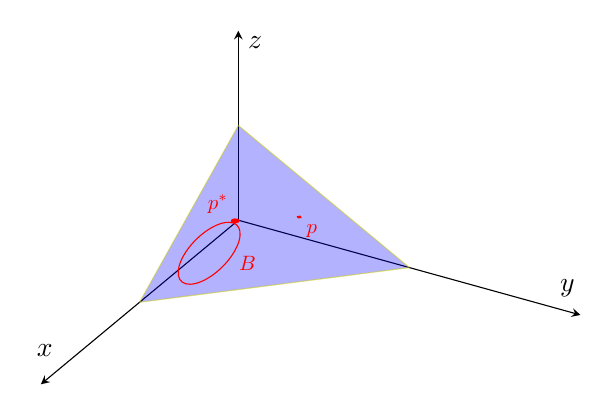
\begin{tikzpicture}
		\begin{axis}[
				axis lines = middle,
				xlabel = $x$,
				ylabel = $y$,
				zlabel = $z$,
				xtick=\empty,
				ytick=\empty,
				ztick=\empty,
				xmin = 0, xmax = 2,
				ymin = 0, ymax = 2,
				zmin = 0, zmax = 2,
				view={120}{45}
			]
			\addplot3[
				patch,
				patch type=triangle,
				opacity=0.5,
				fill opacity=0.3,
				color=blue,
			] coordinates {
					(1, 0, 0)
					(0, 1, 0)
					(0, 0, 1)
				};

			% Draw a patch B on the surface 
			\node[red, scale=0.75] at (axis cs: 0.5, 0.25, 0.25) [below right] {$B$};
			\draw[red] (axis cs: 0.5, 0.25, 0.25) ellipse [x radius=0.2, y radius=0.2, rotate around={45:(axis cs: 0.5, 0.25, 0.25)}];

			% Plot random point p outside B 
			\draw[red, fill] (axis cs: 0.25, 0.5, 0.5) circle (0.01) node[below right, scale=0.75] {$p$};

			% Plot distinct point q 
			\draw[red, fill] (axis cs: 0.1, 0.04, 0.1) circle (0.02) node[above left, scale=0.75] {$p^*$};
		\end{axis}

	\end{tikzpicture}
\end{center}

\begin{tbox}{\textbf{Sanov's Theorem:} Let $B$ be an open subset of the space of all PMF on $\{1, \dots, s\}$. Then
		\[\lim_{n \to \infty} \frac{1}{n}\log \P(\hat p \in B) = -\inf_{q \in B} D(q \parallel p)\]
		Further, if $p^* = \argmin_{q \in B} D(q \parallel p)$ is unique, then
		\[\lim_{n \to \infty} \P(\norm{\hat p - p^*} > \ep \; | \; \hat p \in B) = 0 \quad \forall \ep > 0\]
		where $\norm{\hat p - p^*}$ is any metric, say $\norm{\hat p - p^*} = \max_{x \in \{1, \dots, s\}} \abs{\hat p_x - p_x}$}
	\emph{Proof:}
\end{tbox}

\tbf{Remark:} What if $p \in B$? Then $\inf_{q \in B} D(q \parallel p) = 0$, so
\[\frac{1}{n} \log \underbrace{e^{-o(n)}}\P(\hat p \in B) = 0\]


\section{Feb 5}
\tbf{Recall (Sanov's Theorem):} For $B$ open,
\begin{enumerate}
	\item \[\lim_{n \to \infty} \frac{1}{n} \log \P(\hat p_{x_1, \dots, x_n} \in B) = -\inf_{q\in B} D(q \parallel p)\]
	\item If $\exists ! \; p^* = \argmin_{q \in \bar B} D(q \parallel p)$, then
	      \[\lim_{n \to \infty} \P(\norm{\hat p - p} > \ep \; | \; \hat p \in B) = 0 \quad \forall \ep >0 \]
\end{enumerate}


\begin{center}
	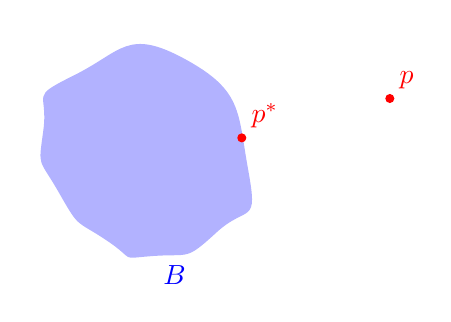
\begin{tikzpicture}
		% Draw a blob
		\fill[blue, opacity=0.3] plot[smooth cycle, tension=1.2] coordinates {
				(0, 0)
				(0.8, 0.3)
				(1.2, 1.1)
				(0.4, 2.5)
				(-1, 2.3)
				(-1.4, 1.6)
				(-1.2, 0.8)
				(-0.6, 0.2)
			};

		\draw[fill, red] (1.12, 1.5) circle (0.05) node[above right] {$p^*$};
		\draw[fill, red] (3, 2) circle (0.05) node[above right] {$p$};

		\node[blue, below right] at (0, 0) {$B$};
	\end{tikzpicture}
\end{center}

This leads to some interesting questions:
\begin{enumerate}
	\item Why is $p^*$ drawn on the boundary?
	\item Is there a case when $p^*$ lies in the interior?
\end{enumerate}

For the second: yes, if $p \in B$ (in which case $p$ is the global minimizer of $D(q \parallel p)$).

For the first, it suffices to show that since $D(q \parallel p)$ is a convex function, on any set $B$ with $p \notin B$, the minimizer $p^*$ must lie on the boundary.

\emph{Example:}

\begin{center}
	\begin{tikzpicture}
		\begin{axis}[
				axis lines = middle,
				xlabel = $x$,
				ylabel = $y$,
				xtick=\empty,
				ytick=\empty,
				clip=false
			]
			\addplot[blue, domain=-4:1] {x^2 + 1};
			\addplot[red, dashed, domain=1:2] {x^2 + 1};
			\addplot[blue, domain=2:4] {x^2 + 1};


			\addplot[red, ultra thick, dashed, domain=1:2] {0} node[below] {$B$};

			\coordinate (A) at (0, 1);

			\coordinate (B) at (1, 2);

		\end{axis}
		\draw[blue, fill] (A) circle (0.1) node[above left] {$p$};
		\draw[red] (B) circle (0.1) node[above] {$p^*$};
	\end{tikzpicture}
\end{center}

\emph{Example:} $B = \{q \; | \; \exists x: \abs{q_x - p_x} > 0\}$

By Sanov,
\[\P(\hat p_n \in B) \approx \exp(-n \inf_{q\in B} D(q \parallel p)) \leq e^{-n/2} < 10\%\]

Now let's prove the claim:
\begin{proof}
	\emph{Proof:}
	\begin{align*}
		F(q)                                              & = D(q \parallel p) = \sum q_x \log \frac{p_x}{q_x} \\
		                                                  & = \sum q_x \log q_x - \sum q_x \log p_x            \\
		\frac{\partial F}{\partial q_x}                   & = \log q_x + 1 - \log p_x                          \\
		\frac{\partial^2 F}{\partial q_x \, \partial q_y} & = \begin{cases}
			                                                      1/q_x & x = y    \\
			                                                      0     & x \neq y
		                                                      \end{cases}                                 \\
		H                                                 & = \begin{pmatrix}
			                                                      \frac{1}{q_1}                             \\
			                                                       & \frac{1}{q_2}                          \\
			                                                       &               & \ddots                 \\
			                                                       &               &        & \frac{1}{q_s}
		                                                      \end{pmatrix}
	\end{align*}
	But $\forall v \in \R^s$, $v^T H v = \sum v_i^2 \frac{1}{q_i} \geq 0 \implies H$ is positive semi-definite. Hence $F$ is convex.
\end{proof}

\subsection{Back to Gibbs' Heat Bath}
Recall the original motivating example where $X_1, \dots, X_n \sim p$, and $\frac{1}{n} \sum_{i=1}^{n} \Ec(X_i) = \theta$.

Previously, we showed that $\theta = \frac{1}{n} \sum_{i=1}^{n} \Ec(X_i) = \E_{\hat p} [\Ec(X)]$.

Now consider the set $B = \{q \; | \; \E_q [\Ec(X)] > \theta\}$ and define $\Omega = \{q: \E_q [\Ec(X)] = \theta\}$.

\begin{center}
	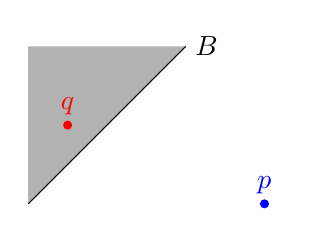
\begin{tikzpicture}
		\fill[opacity=0.3] plot coordinates {
				(0, 0)
				(2, 2)
				(0, 2)
			};

		\draw[fill, red] (0.5, 1) circle (0.05) node[above] {$q$};
		\draw (0, 0) -- (2, 2) node[right] {$B$};

		\draw[fill, blue] (3, 0) circle (0.05) node[above] {$p$};
	\end{tikzpicture}
\end{center}
Imagine we observe some sample with energy higher than expected (i.e. $q \in B$). What is the probability of this occurring?

By Sanov, in order to find $\inf_{q \in B} D(q \parallel p)$, it suffices to find $p^*$ such that $D(p^* \parallel p) = \inf_{q \in B} D(q \parallel p)$.

In the past, we used Lagrange multipliers to confirm our solution is in the \tbf{exponential family}
\[p_x^* = \frac{1}{Z_{\lambda}} p_x \exp(\lambda \Ec(x)) \quad \forall x\]
for some $\lambda$.

\emph{Example of Exponential Family:} $\mathcal{N}(\mu, \sigma^2)$ has PDF $\frac{1}{Z} e^{-\frac{(x- \mu)^2}{2\sigma^2}}$

If instead we had many constraints $\E_{\hat p} [\Ec_i(X)] = \theta_i$ for $i = 1, \dots, k$, we found minimizer
\[p^* = \frac{1}{Z_{\lambda_1 \dots \lambda_k}} p_x \exp(\lambda_1 \Ec_1(x) + \dots + \lambda_k \Ec_k(x))\]
where we found $\lambda_1, \dots, \lambda_k$ using Lagrange multipliers to satisfy the constraints and
\[Z_{\lambda_1\dots \lambda_k} = \sum_x p_x \exp(\lambda_1 \Ec_1(x) + \lambda_k \Ec_k(x))\]

These must also satisfy:
\begin{enumerate}
	\item $\frac{\partial}{\partial \lambda_k} \log Z_k = \E_{\lambda}[\Ec_k(X)]$
	\item $\frac{\partial^2}{\partial \lambda_k \lambda_l} \log Z_k = \text{Cov}_{\lambda}(\Ec_k(X), \Ec_l(X)) \quad \forall k, l$
	\item $\log Z_k$ is a convex function of $\lambda$ and it is strictly convex unless $\exists \alpha = (\alpha_1, \dots, \alpha_k)$ such that $\alpha \neq 0$ and $\sum_{k=1}^c \alpha_k \Ec_k(x) = \text{const} \quad \forall x$
	\item $\log Z_{\lambda} - \sum \lambda_k \theta_k$ is convex in $\lambda$ and minimized when $\E_{\lambda}[\Ec(X)] =\theta_k$
\end{enumerate}

\section{Feb 7}
Last time, we defined the set
\[B = \{q: \E_q \Ec(X) < \theta\}\]

For $p \notin B$ known, we know that the minimizer $p^* = \argmin_{q\in B} D(q \parallel p)$ lies on the boundary of $B$, $\Omega = \{q: \E_q [\Ec(X)] = \theta\}$.

Using Lagrange Multipliers, we found
\[p_x^* = \frac{1}{Z_{\lambda}} p_x  e^{\lambda \Ec(x)} \quad \forall x\]
with
\[Z_{\lambda} = \sum_{x=1}^{s} p_xe^{\lambda \Ec(x)}\]

Now, we want to find $\lambda = (\lambda_1, \dots, \lambda_s)$ that satisfies
\[\E_{p^*}[\Ec(X)] = \theta \iff \sum p_x^* \Ec(x) = \theta \iff \sum \frac{1}{Z_{\lambda}} p_x e^{\lambda \Ec(x)} \Ec(x) = \theta\]

\begin{tbox}{\textbf{Proposition:}
		\begin{enumerate}
			\item $\frac{\partial}{\partial \lambda_k} \log Z_{\lambda} = \E_{\lambda}[\Ec_k(X)] \quad \forall k=1, \dots, c$
			\item $\frac{\partial^2}{\partial \lambda_k \, \partial \lambda_l} \log Z_{\lambda} = \Cov_{\lambda} (\Ec_k(X), \Ec_l(X)) \quad \forall k,l$
			\item $\log Z_{\lambda}$ is convex in $\lambda$ and, in general, strictly convex (unless the equations $\left\{\E_{p^*} \Ec_k(X) = \theta_k\right\}_{k=1}^c$ are redundant, i.e. $\not\exists b_1, \dots b_c \neq (0, \dots, 0)$)
			\item Assuming (3), the function
			      \[\log Z_{\lambda} - \sum_{k=1}^{c} \lambda_k \theta_k\]
			      is in general strictly convex and is minimized when
			      \[\E_{\lambda}[\Ec_k(X)] = \theta_k \quad \forall k\]
			      (i.e. at exactly the $\lambda$ that we need to find)
		\end{enumerate}
	}
	\emph{Proof:}

	\begin{enumerate}
		\item  \begin{align*}
			      \frac{\partial }{\partial \lambda_k} \log Z_{\lambda} & = \frac{1}{Z_k} \cdot \frac{\partial }{\partial \lambda_k} Z_{\lambda}                                                                       \\
			                                                            & = \frac{1}{Z_{\lambda}} \cdot \frac{\partial }{\partial \lambda_k} \left[\sum p_x e^{\lambda_1 \Ec_1(x) + \dots + \lambda_c \Ec_c(x)}\right] \\
			                                                            & = \frac{1}{Z_{\lambda}} \cdot \sum_x p_x e^{\lambda_1 \Ec_1(x) + \dots + \lambda_c \Ec_c(x)} \cdot \Ec_k(x)                                  \\
			                                                            & = \frac{1}{Z_{\lambda}}  \cdot \sum_x p_x \Ec_k(x) e^{\lambda \Ec(x)}                                                                        \\
			                                                            & = \sum_x p_x^* \Ec_k(x)                                                                                                                      \\
			                                                            & = \E_{p^*}[\Ec_k(X)] = \E_{\lambda}[\Ec_k(X)]
		      \end{align*}

		      \tbf{Remark:} We write $\E_{\lambda}$ instead of $\E_{p^*}$ just to emphasize that this is a function of $\lambda$

		\item

		      \begin{exercise}
			      \textbf{Exercise:}  Email the proof to oanh\_nguyen1@brown.edu for bonus points.

			      \div

			      \emph{Proof:}  In part 1, we showed that $\frac{\partial}{\partial \lambda_k} \log Z_{\lambda} = \E_{\lambda}[\Ec_k(X)]$. Hence, it suffices now to show
			      \[\frac{\partial}{\partial \lambda_l} \E_{\lambda}[\Ec_k(X)] = \Cov_{\lambda}(\Ec_k(X), \Ec_l(X))\]

			      \textcolor{red}{TODO}
		      \end{exercise}

		\item \[H(\lambda_1, \dots, \lambda_c) = \begin{pmatrix}
				      \frac{\partial^2}{\partial \lambda_k\, \partial \lambda_l} \log Z_{\lambda}
			      \end{pmatrix}_{c \times c}\]

		      We need to show $\forall v \neq \vec 0$,
		      \[v^T H v = \sum_{k, l}v_k v_l H_{kl} \geq 0 \implies \log_Z \text{ convex}\]

		      But
		      \begin{align*}
			      \sum v_k v_l H_{kl} & = \sum v_k v_l \Cov(\Ec_k(X), \Ec_l(X))     \\
			                          & = \Var\left(\sum v_k \Ec_k(X)\right) \geq 0
		      \end{align*}
		      since
		      \[\sum v_k v_l \Cov(Y_k, T_l) = \Var\left(\sum v_k y_k\right)\]

	\end{enumerate}

\end{tbox}

\section{Feb 10}
Let $B = \{q: \E_q[\Ec(X)] < \theta\}$. Suppose we have two constraints
\begin{itemize}
	\item $\E_{\hat p} [\Ec_1(X)] = \theta_1$
	\item $\E_{\hat p} [\Ec_2(X)] = \theta_2$
\end{itemize}
and we know
\begin{itemize}
	\item $\E_p [\Ec_1(X)] > \theta_1$
	\item $\E_p [\Ec_2(X)] > \theta_2$
\end{itemize}

Then we can tighten
\[B = \{q: \E_q[\Ec_1(X]]< \theta_1, \; \E_q[\Ec_2(X)] > \theta_2\}\]
which updates our partition of the space from:

\begin{center}
	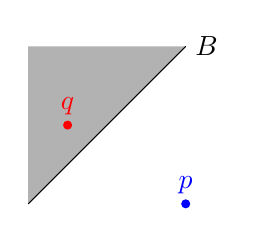
\begin{tikzpicture}
		\fill[opacity=0.3] plot coordinates {
				(0, 0)
				(2, 2)
				(0, 2)
			};

		\draw[fill, red] (0.5, 1) circle (0.05) node[above] {$q$};
		\draw (0, 0) -- (2, 2) node[right] {$B$};

		\draw[fill, blue] (2, 0) circle (0.05) node[above] {$p$};
	\end{tikzpicture}
	\hspace{1cm}
	\begin{tikzpicture}
		\node at (0, 0) {};
		\node at (0,1) {$\longrightarrow$};
	\end{tikzpicture}
	\hspace{1cm}
	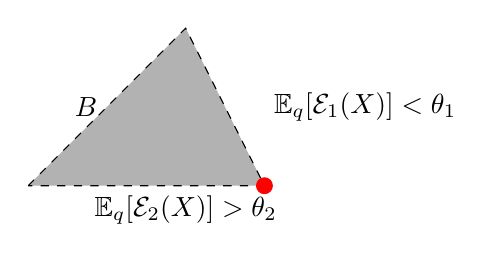
\begin{tikzpicture}
		\fill[opacity=0.3] plot coordinates {
				(0, 0)
				(2, 2)
				(3, 0)
			};

		\draw[dashed] (0, 0) -- (2, 2) -- (3, 0) -- cycle;

		\node[left] at (1, 1) {$B$};
		\node[below] at (2, 0) {$\E_q[\Ec_2(X)] > \theta_2$};
		\node[right] at (3, 1) {$\E_q[\Ec_1(X)] < \theta_1$};

		\draw[fill, red] (3, 0) circle (0.1);
	\end{tikzpicture}
\end{center}
which tells us
\[\Omega = \{q: \E_q[\Ec_1(X)] = \theta_1, \quad \E_q[\Ec_2(X)] = \theta_2\} \]

We already know what to do if $p^* \in \Omega$, so consider just one constraint:
\[\E_q[\Ec_2(X)] = \theta_2\]

We can easily find $p_2^*$ WRT this constraint:
\begin{align*}
	B_2      & = \{q: \E_q[\Ec_2(X)] > \theta_2\}          \\
	\Omega_2 & = \{q: \E_q[\Ec_2(X)] = \theta_2\}
	p_2^*    & = \argmin_{q \in \Omega_2} D(q \parallel p)
\end{align*}

Further, we know if $p_2^* \in \bar B$, then $p^* = p_2^*$ and we are done.

Otherwise, we can just try again using the first constraint to find $p_1^*$. If $p_1^* \in \bar B$, then $p^* = p_1^*$ and we are done.

What if we get unlucky both times and $p_1^*, p_2^* \notin \bar B$?

\begin{tbox}{\textbf{Claim:} Because of convexity, if $p_1^*, p_2^* \notin \bar B$, then $p^* \in \Omega$}
	\emph{Proof:}

	\begin{center}
		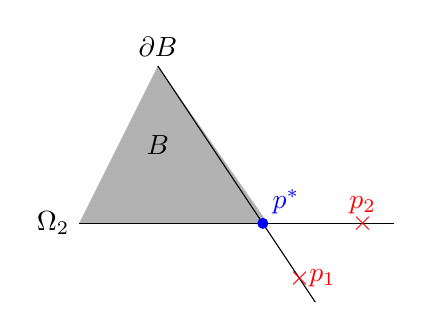
\begin{tikzpicture}
			\fill[opacity=0.3] plot coordinates {
					(0, 0)
					(1, 2)
					(2.4, 0)
				};

			\draw[name path=A] (4, 0) -- (0, 0)
			node[pos=0.1, red] {$\times$}
			node[pos=0.1, red, above] {$p_2$}
			node[left] {$\Omega_2$};

			\draw[name path=B] (3, -1) -- (1, 2)
			node[pos=0.1, red] {$\times$}
			node[pos=0.1, red, right] {$p_1$}
			node[above] {$\partial B$};

			\node at (1, 1) {$B$};

			\fill [blue, name intersections={of=A and B, by=x}] (x) circle (2pt) node[above right] {$p^*$};
		\end{tikzpicture}
	\end{center}


	WLOG, $p^* \in \Omega_1$ so let $\tilde p = [p^*, p_1^*] \cap \Omega \implies \tilde p \in \Omega$.
	\begin{center}
		\begin{tikzpicture}
			\draw[name path=A] (4, 0) -- (0, 0)
			node[pos=0, right] {$\{q: \E_q[\Ec_2(X)] = \theta_2\}$};

			\draw[name path=B] (3, -1) -- (1, 2)
			node[pos=0.7, red] {$\times$}
			node[pos=0.7, red, above right] {$p^*$}
			node[pos=0.1, red] {$\times$}
			node[pos=0.1, red, above right] {$p_1$};

			\fill [blue, name intersections={of=A and B, by=x}] (x) circle (2pt) node[above right] {$\tilde p$};

		\end{tikzpicture}
	\end{center}

	Then the $\tilde p$ should have been $p^*$ (contradiction.)

	Or
	\[\tilde p = \lambda p^* + (1- \lambda)p_{\perp}^* \quad \lambda (0, 1)\]
	so
	\[D(\tilde p \parallel p) \leq \lambda D(p^* \parallel p) + (1-\lambda) D(p_{\perp}^* \parallel p)\]
	but $D(p^* \parallel p)$ and $D(p_{\perp}^* \parallel p)$ are the smallest among the points while $D(\tilde p \parallel p)$ should be the largest. Contradiction.
\end{tbox}

\subsection{Information Point of View for Shannon Entropy}
In the following section, let $\log = \log_2$

Here, \tbf{Shannon Entropy} ``measures the minimal number of bits needed to encode a message optimally''.

For example, let $X_1, \dots, X_n \sim \{1, 2\}$ with $p= (p_1, p_2)$ and $p_2 = 1-p_1$.

As before, let $\hat p_1 = \frac{\#\{i: X_i = 1\}}{n}$ and $\hat p_2 = 1 - \hat p_1$.

\tbf{Question:} What is the probability of any particular sequence? (say $\hat p_1 \approx p_1, \hat p_2 \approx p_2$)

\emph{Answer:}
\begin{align*}
	\P(X_1= x_1, \dots, X_n = x_n) & = p_1^{\hat p_1 n} p_2^{\hat p_2 n}             \\
	                               & \approx p_1^{p_1 n} p_2^{p_2 n}                 \\
	                               & = 2^{n(\log p_1) p_1} \cdot 2^{n(\log p_2) p_2} \\
	                               & = 2^{-nH(p)}
\end{align*}
and this makes some sense: if we have no information, we would expect the probability of any sequence to be $2^{-n}$.

\section{Feb 12}

Let $\{X_i\}_{i=1}^n \sim \{0, 1\}$ with $p = (p_0, p_1) = (p_0, 1 - p_0)$. The Shannon Entropy is
\begin{align*}
	H(p) & = -\sum p_x \log p_x                                \\
	     & = -p_0 \log p_0 - p_1 \log p_1                      \\
	     & = -p_0 \log p_0 - (1 - p_0) \log (1 - p_0) = F(p_0)
\end{align*}
for some function $F$.

\begin{center}
	\begin{tikzpicture}
		\begin{axis}[
				axis lines = middle,
				xlabel = $p_0$,
				ylabel = $H(p)$,
				xtick={1/2, 1},
				ytick={1},
				xmin = 0, xmax = 1.5,
				ymin = 0, ymax = 1.5,
				clip=false,
				axis equal
			]
			\addplot[blue, domain=0:1.5] {-x * log2(x) - (1 - x) * log2(1 - x)};
			\node at (axis cs: 0.5, 1) {$\bullet$};
		\end{axis}
	\end{tikzpicture}
\end{center}

What is the relationship between the Shannon Entropy and the KL-Divergence?

\begin{align*}
	D(p \parallel h) & = \sum p_x \log \frac{p_x}{h_x}         \\
	                 & = \sum p_x \log p_x - \sum p_x \log h_x \\
	                 & = -H(p) - \log \frac{1}{s}
\end{align*}
for $h \sim \text{Unif}(1, s)$. Hence, up to a constant, $H(p) \approx D(p \parallel \text{Unif}\{1, \dots, s\})$.

And indeed this justifies that $H(p)$ has its max at $1/2$ when $p = (1/2, 1/2)$.

This also explains what we found last class: we only need $2^{nH(p)}$ bits rather than $2^n$ because in the worst case, $H(p) = 1 \implies 2^{n\cdot 1} = 2^n$.

\subsection{Source Coding}
More generally, we can take $X = (X_1, \dots, X_n) \sim p$ on states $\{1, \dots, t\}$ for $t = 2^n$.

Let $C: \{1, \dots, t\} \to \{0, 1\}^*$ be a \tbf{source code} where $\{0, 1\}^*$ is the set of finite non-empty strings of 0s and 1s.

We let $\abs{C(x)}$ denote the length of the code. In general, we want $\abs{C(x)}$ to be small across different $x$.

\tbf{Example:} A trivial code is the identity: $C(x) = x$ for all $x$. For $p = 1/2$, this is the best we can do.

If, however, $p = (0.99, 0.01)$ we can do better in expectation.

\tbf{Prefix:} A \emph{prefix code} is a code $C$ for which $C(x)$ is not a prefix for $C(\tilde x)$ for any $x \neq \tilde x$.

\emph{Example:}

\qquad \begin{tabular}{c|cc}
	$x$ & $C(x)$ & $C'(x)$ \\ \hline
	1   & 0      & 0       \\
	2   & 1      & 10      \\
	3   & 00     & 11      \\ \hline
\end{tabular}

Here, $C$ is not a prefix because under $C$, if we are trying to encode 0100, we do not know if it should be 120 or 1211. However, $C'$ is a prefix because there is no ambiguity.

\tbf{Remark:} Being a prefix is not necessary for unique decoding. For example,

\qquad \begin{tabular}{c|c}
	$x$ & $C(x)$ \\ \hline
	1   & 0      \\
	2   & 01     \\
	3   & 011    \\ \hline
\end{tabular}

is not a prefix but any string can be uniquely decoded by looking back.

\tbf{Question:} What is the minimal $(\abs{C(x)})_x$ (i.e. $C = \argmin \E_p \abs{C(x)} = \sum p_x \abs{C_x}$) where $C$ is a prefix code?

If we simply return the message, every encoded message is of equal length so $C$ is a prefix code of expected length $n$. Can we do better?

\begin{proposition}
	\textbf{Proposition (Kraft-McMillan Inequality):} For all prefix codes $C$,
	\[\sum_{x=1}^t 2^{-\abs{C(x)}} \leq 1\]
	and for any code lengths $\ell_1, \dots, \ell_t$ such that
	\[\sum_{x=1}^t 2^{-\ell_x} \leq 1\]
	there exists a a prefix code $C$ with $\abs{C_x} = \ell_x$ (letting $C_x = C(x)$).
\end{proposition}

\emph{Example:} In the non-prefix example, we say $\ell_1 = 1, \ell_2 = 2, \ell_3 = 3$ so
\[\sum_{x=1}^t 2^{-\ell_x} = 2^{-1} + 2^{-2} + 2^{-3} \leq 1\quad \checkmark \]

We can visualize this as a tree:
\begin{center}
	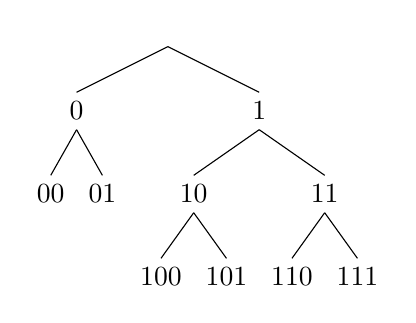
\begin{tikzpicture}
		\Tree [.{}
				[.0 \node{00}; \node{01};]
				[.1
						[.{10} \node{100}; \node{101};]
						[.{11} \node{110}; \node{111};]]
		]
	\end{tikzpicture}
\end{center}


We will see next time that the optimal code $C^*$ satisfies $H(p) \leq \E\abs{C^*(X)} \leq H(p)$

\section{Feb 14}
\tbf{Motivation:} Let $p = (p_1, p_2)$ be a distribution on $\{0, 1\}$ ($s = 2$).

Sample $(X_1, \dots, X_n)$ corresponding to $n$ bits. Hence, there are $2^n$ possible sequences.

We can design a prefix code $C: \{0, 1\}^n \to \{0, 1\}^*$.

\emph{Example:} For $n = 3$,

\qquad\begin{tabular}{c|c}
	$X_1X_2X_3$ & $C(X_1X_2X_3)$ \\ \hline
	000         & 00             \\
	001         & 01             \\
	\vdots                       \\
	111
\end{tabular}

with $\E_p[\abs{C_x}] \approx H(p)n$. And indeed this is a prefix since every image is the same length.

We know that for the identity code, $C(x) = x$, $\E_p [\abs{C_{(X_1, \dots, X_n)}}] = n$.

\begin{proposition}
	\textbf{Theorem:} Let $\vec X \sim \vec p$. For the optimal code $C^* = \argmin_{C \text{ prefix}} \E_{\vec p} [\abs{C(X)}]$,
	\[H(\vec p) \leq \abs{\E_{\vec p}} C^*(X) \leq H(\vec p ) + 1\]
\end{proposition}

\tbf{Remark: }In our example, $\vec X = (X_1, \dots, X_n), \quad X_i \iid p$ so
\[H(\vec p) \leq \E_{\vec p} \abs{C(X)} \leq H(\vec p) + 1\]
where $\vec p = p \otimes \dots \otimes p$.

\begin{tbox}{\textbf{Claim:}
		\begin{enumerate}
			\item $H(\vec p) = nH(p)$.
			\item $H(X, Y) = H(X) + H(Y)$ if $X, Y$ independent
		\end{enumerate} }
	\emph{Proof:}
	1. Follows as a corollary from (2).

	\div

	2. Let $X$ take values $\{x_1, \dots, x_A\}$ and $Y$ take values $\{y_1, \dots, y_B\}$.

	Then
	\begin{align*}
		H(X, Y) & = -\sum_{i=1}^{AB} p_{i} \log p_{i}                                                        \\
		        & = -\sum_{x=1}^A \sum_{y=1}^B p_{xy} \log p_{xy}                                            \\
		        & = -\sum_x \sum_y p_x q_y \log p_x q_y \qquad (X, Y \text{ independent})                    \\
		        & = -\sum_x \sum_y p_x q_y \log p_x + p_x q_y \log q_y                                       \\
		        & = -\sum_y p_y \sum_x p_x \log p_x - \sum_x p_x \sum_y q_y \log q_y \qquad (\text{Tonelli}) \\
		        & = \sum_y q_y H(x) + \sum_x p_x H(y)                                                        \\
		        & = H(X) + H(Y) \qed
	\end{align*}
\end{tbox}

Hence,
\[nH(p)\leq \E{\abs{C(X)}} \leq nH(p) + 1\]

In particular, our propositions from earlier in the week follow immediately. Most importantly, we have confirmed that we indeed only need $2^{nH(p)}$ bits to encode a message.

At last, we are ready to actually prove the theorem:

\begin{tbox}{\textbf{Theorem:} Let $\vec X \sim \vec p$. For the optimal code $C^* = \argmin_{C \text{ prefix}} \E_{\vec p} [\abs{C(X)}]$,
		\[H(\vec p) \leq \abs{\E_{\vec p}} C^*(X) \leq H(\vec p ) + 1\]}
	\emph{Proof:} Let $X \sim p$.

	\begin{enumerate}
		\item $H(p) \leq \E_p \abs{C(X)}$

		      Let $\ell_x = \abs{C_x}$. Then
		      \begin{align*}
			      \E\abs{C(X)} - H(p) & = \sum p_x \ell_x + \sum p_x \log p_x                                                       \\
			                          & =  \sum p_x \log(2^{\ell_x} p_x)                                                            \\
			                          & = \sum p_x \log \frac{p_x}{2^{-\ell_x}}                                                     \\
			                          & = \sum p_x \log \frac{p_x}{2^{-\ell_x} \cdot \frac{\sum_y 2^{-\ell_y}}{\sum_y 2^{-\ell_y}}} \\
		      \end{align*}

		      Let $S = \sum_x 2^{-\ell_x}$. By Kraft-McMillan, $S \leq 1$ so

		      \begin{align}
			       & = \sum_x p_x \log \frac{p_x}{q_x S}                   \\
			       & = \sum_x p_x \log \frac{p_x}{q_x} - \sum_x p_x \log S \\
			       & = D(p \parallel q) - \log S \geq 0
		      \end{align}

		\item $\E\abs{C^*(X)} \leq H(p) + 1$.

		      It suffices to show $\exists C$ prefix such that
		      \[\E_p\abs{C(X)} \leq H(p) + 1\]

		      In fact, our Part I gives us a place to start: We would like to find $\ell_x$ such that $q_x \propto 2^{-\ell_x} \approx p_x$. Hence, let $\ell_x = \left\lceil \log_2 \frac{1}{p_x} \right\rceil$.

		      Now, we just need to show $\exists C$ prefix such that $\ell_x = \abs{C_x}$. But by Kraft-Mcmillan, it suffices to show $\sum_x 2^{-\ell_x} \leq 1$.

		      With a little more work, we can show this exactly. Heuristically, if we did not need to round to get an integer $\ell_x$, we would have $H(p)$ exactly. Rounding, we get $H(p) + 1$.
	\end{enumerate}
\end{tbox}

\section{Feb 19}
\tbf{Example:} $s = 3$ with $p = (1/2, 1/4, 1/4)$.

Then
\[H(p) = \sum p_x \log \frac{1}{p_x} = \frac{1}{2} \log 2 + \frac{1}{4} \log 4 + \frac{1}{4} \log 4 = \frac{3}{2}\]

If we want to encode $X_1\cdots X_n$, we have $3^n$ possible sequences. We would naturally like to design a prefix code $C$ with length $\ceil{\log_2 \frac{1}{p_x}}$.

One way is via block coding. We first choose the lengths:

\qquad \begin{tabular}{ccc}
	$X_1$ & $p_x$ & $\ell_x = \ceil{\log_2 \frac{1}{p_x}}$ \\\hline
	$1$   & $1/2$ & $1$                                    \\
	$2$   & $1/4$ & $2$                                    \\
	$3$   & $1/4$ & $2$
\end{tabular}

If we say $C(1) = 0$, then we can prune the resulting tree for all other encodings:
\begin{center}
	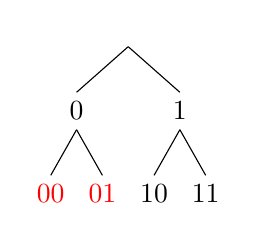
\begin{tikzpicture}
		\Tree [.{}
				[.0 \node[red]{00}; \node[red]{01};]
				[.1 \node{10}; \node{11};]
		]
	\end{tikzpicture}
\end{center}
which naturally leads us to a full prefix code:

\qquad \begin{tabular}{ccc}
	$X_1$ & $C(x)$ \\\hline
	1     & 0      \\
	2     & 10     \\
	3     & 11
\end{tabular}

\tbf{Example:} Now consider $s = 3$, $p = (1/3, 1/3, 1/3)$. Then $H(p) = \log 3 \approx 1.58$. So

For $n = 1$,

\qquad \begin{tabular}{cccc}
	$x$ & $p(x)$ & $\ell_x$               & $C(x)$ \\\hline
	$1$ & $1/3$  & $\ceil{\log_2(3)} = 2$ & 0      \\
	$2$ & $1/3$  & $2$                    & 10     \\
	$3$ & $1/3$  & $2$                    & 11
\end{tabular}

with
\[\E\abs{C_x} = \frac{2}{3}(2) + \frac{1}{3}(1) = \frac{5}{3}\]

But with $n=2$, we have $3^2 = 9$ possible sequences. Looking at the tree, we can choose a reasonable minimal encoding:

\begin{center}
	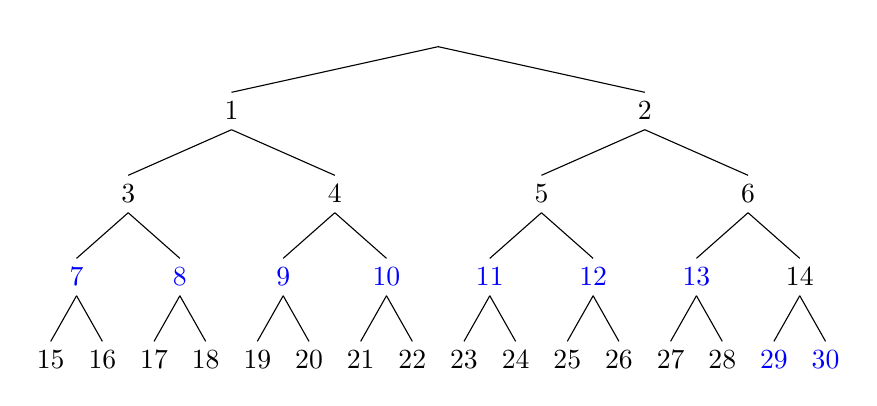
\begin{tikzpicture}
		\Tree [.{}
				[.{1}
						[.{3} [.\node[blue]{7}; \node{15}; \node{16};]
								[.\node[blue]{8}; \node{17}; \node{18};]]
						[.{4} [.\node[blue]{9}; \node{19}; \node{20};]
								[.\node[blue]{10}; \node{21}; \node{22};]]]
				[.{2}
						[.{5} [.\node[blue]{11}; \node{23}; \node{24};]
								[.\node[blue]{12}; \node{25}; \node{26};]]
						[.{6} [.\node[blue]{13}; \node{27}; \node{28};]
								[.{14} \node[blue]{29}; \node[blue]{30};]]]]
	\end{tikzpicture}
\end{center}

which gives
\qquad \begin{tabular}{cccc}
	$x$ & $p(x)$ & $\ell_x$ & $C(x)$ \\\hline
	11  & $1/3$  & 4        & 000    \\
	12  &        &          & 001    \\
	13  &        &          & \vdots \\
	21                               \\
	22                               \\
	23                               \\
	31  &        &          & 110    \\
	32  &        &          & 1110   \\
	33  &        &          & 1111
\end{tabular}

which has
\[\E\abs{C_x} = \frac{7}{9}(3) + \frac{2}{9}(4) \approx 3.222 = 1.611 \cdot 2\]
which means we use 1.611 bits per signal.

If $n \to \infty$, then the best prefix code has an average $H(p)$ bits per symbol.

\chapter{Statistical Inference}
\section{Feb 19}
\subsection{Probability Estimation}
\tbf{Motivation:} Let $X_1, X_2, \, \dots,\, X_n \iid P_{\theta}$. We want to estimate $\theta$.

\emph{Example:} If $X_1, \dots, X_n \sim \mathcal{N}(\mu, \sigma^2)$, then $\theta = (\mu, \sigma)$.

\tbf{Unbiased Estimation:} Suppose $\hat \theta = \hat \theta(x_1, \dots, x_n)$ is an estimation of $\theta$. If $\E[\hat \theta] = \theta$, we say $\hat \theta$ is \emph{unbiased.}

\tbf{Example:} Let $X_1, \dots, X_n \sim \Nc(\mu, \sigma^2)$.
\begin{itemize}
	\item $\hat \mu = \frac{1}{n}(X_1 + \dots + X_n)$ is unbiased since
	      \[\E[\hat \mu] = \frac{1}{n} \sum \E[X_i] = \frac{1}{n}(n)(\mu) = \mu\]
	\item What is an unbiased estimator for $\sigma^2$? We know $\sigma^2 = \E[X^2] - (\E X)^2 = \E[(X - \mu)^2]$ so
	      \[\hat \sigma^2 = \frac{1}{n-1} \sum_{i=1}^{n} (X_i - \hat \mu)^2 \]

	\item In fact, $\hat{\hat{\sigma^2}} = \frac{1}{n} \sum_{i=1}^n (X_i - \hat \mu)^2$ is a biased estimator:

	      \begin{proof}
		      \emph{Proof:} WLOG $\mu = 0$ (else $Y_i = X_i - \mu \sim \Nc(0, \sigma^2) \implies \hat \mu_X = \hat \mu_Y - \mu$).

		      Then $\sigma^2 = \E[X^2]$ so
		      \begin{align*}
			      \hat \mu          & = \frac{1}{n} \sum X_i                                                                                               \\
			      \hat \sigma^2     & = \frac{1}{n-1} \sum (X_i - \hat \mu)^2
			      \E[\hat \sigma^2] & = \E\left[\frac{1}{n-1} \sum (X_i - \hat \mu)^2\right]                                                               \\
			                        & = \frac{1}{n-1} \sum \E[(X_i - \hat \mu)^2]                                                                          \\
			                        & = \frac{n}{n-1} \E[(X_i - \hat \mu)^2]                                                                               \\
			                        & = \frac{n}{n-1} \E\left[\left(X_i - \frac{X_1 + \dots + X_n}{n}\right)^2\right]                                      \\
			                        & = \E\left[\left(\frac{n-1}{n}X_1 - \frac{1}{n} X_2 \cdots - \frac{1}{n} X_n\right)^2\right]                          \\
			                        & = \E\left[\left(\frac{n-1}{n}\right)^2 X_1^2 + \sum_{i=2}^{n} \frac{1}{n^2} X_1^2 + 2 \sum_{i\neq j} X_i X_j \right] \\
			                        & = (\frac{n-1}{n})^2 \E[X_1^2] + \frac{n-1}{n^2} \E[X_1^2]                                                            \\
			                        & = \frac{(n-1)^2}{n^2} \sigma^2                                                                                       \\
			                        & = \frac{n-1}{n} \sigma^2
		      \end{align*}
		      since for $i \neq j$, $\E[X_i X_j] \overset{X_i \perp X_j}{=} (\E X_i)(\E X_j)$
	      \end{proof}
\end{itemize}

\tbf{Consistent:} We say $\hat \theta_n$ is \emph{consistent} if $\hat \theta_n \longrightarrow \theta$ in some sense as $n \to\infty$. For example,
\begin{itemize}
	\item $\hat \theta_n \overset{a.s.}{\longrightarrow} \theta \implies \P(\lim_{n \to \infty} \hat \theta_n = \theta) = 1$
	\item $\hat \theta_n \overset{P}{\longrightarrow} \theta \implies \forall \ep > 0, \P(\abs{\hat \theta_n - \theta} > \ep) \overset{n\to\infty}{\longrightarrow} 0$
	\item $\hat \theta \overset{\text{mean square}}{\longrightarrow} \theta \implies \E[(\hat \theta_n - \theta)^2] \to 0$.
\end{itemize}

Is $\hat \sigma^2$ consistent in any sense? As we will see, yes. But not trivially so.

\section{Feb 21}

\tbf{Recall:} Let $\theta = \sigma^2$ and take $X_1, X_2, \, \dots,\, X_n \iid p$. Then
\[S_n^2 = \frac{1}{n-1} \sum_{i=1}^{n} (X_i - \bar X)^2\]
is an unbiased estimator for $\sigma^2$.

Further,
\[\hat \sigma_n^2 = \frac{1}{n} \sum_{i=1}^{n} (X_i - \bar X)^2 \]
is a biased estimator for $\sigma^2$.

\tbf{Mean Squared Error (MSE):} $\MSE(\hat \theta_n) = \E \abs{\hat \theta_n - \theta}^2$.

Notice,
\begin{align*}
	\MSE(\hat \theta) & = \E(\hat \theta_n - \theta)^2                                                                                           \\
	                  & = \E(\underbrace{\hat \theta_n - \E \hat \theta_n}_{a} + \underbrace{\E \hat \theta_n + \E\hat \theta_n - \theta}_{b})^2 \\
	                  & = \E (a + b^2)                                                                                                           \\
	                  & = \E a^2 + 2b \underbrace{\E a}_{0} + \underbrace{b^2}_{\text{bias}^2}                                                   \\
	                  & = \Var(\hat \theta) + \text{bias}^2
\end{align*}

\tbf{Example:} Calculate $\MSE(S_n^2)$ vs. $\MSE(\hat \sigma_n^2)$. For simplicity, assume $\mu = 0$,$\sigma^2 = 1$ and $\E_p X^4 = 3$.

\begin{align*}
	\MSE(S_n^2) & = \Var(S_n^2) + \text{bias}^2                         \\
	            & = \Var(S_n^2) \qquad \text{since $S_n^2$ is unbiased} \\
	            & = \E[(S_n^2 - \E S_n^2)^2]                            \\
	            & = \E[(S_n^2 - \sigma^2)^2]                            \\
	            & = \E[(S_n^2 - 1)^2]                                   \\
	            & = \E[S_n^4] - 2\E[S_n^2] + 1                          \\
	            & = \E[S_n^4] - 2 + 1                                   \\
	            & = \E[S_n^4] - 1
\end{align*}

We know
\begin{align*}
	S_n^2 & = \frac{1}{n-1} \left(\sum (X_i - \frac{\sum X_j}{n})\right)^2                                 \\
	      & = \frac{1}{n-1} \sum_{i=1}^n \left(\frac{n-1}{n} X_i - \frac{1}{n} \sum_{j\neq i} X_j\right)^2
\end{align*}

We want
\begin{align*}
	\E[S_n^4] & = \frac{1}{(n-1)^2} \E\left[\sum_i \left(\frac{n-1}{n} X_i - \frac{1}{n} \sum_{j\neq i} X_j\right)^2\right]^2
\end{align*}
up to coefficients, we will only have $X_i^4, X_i^3X_j, X_i^2X_j^2, X_i^2X_jX_k, X_iX_jX_kX_l$ terms in the expansion.

Under expectation, however, only the $X_i^4$ and $X_i^2 X_j^2$ terms will survive.

After a little more work, we find
\begin{align*}
	\MSE(S_n^2)           & = \frac{2}{n -1} \sigma^4  \\
	\MSE(\hat \sigma_n^2) & = \frac{2n-1}{n^2}\sigma^4
\end{align*}
but then $\MSE(\hat \sigma_n^2) < \MSE(S_n^2)$ so even though it is biased, it is a better estimator (in the sense of minimizing MSE).

\subsection{Nonparametric Estimation}
\tbf{Example:} Let $X_1, X_2, \, \dots,\, X_n \iid p$. We want to estimate $p$.

Suppose we have one observation $\hat p_x = \frac{1}{n} \#\{i: X_i = x\}$. How good an estimator is this?

First, is it unbiased? We know that for a set $B$,
\[\hat p(B) = \frac{1}{n}\cdot \#\{i: X_i \in B\} = \sum_{x \in B} \hat p_x\]
and
\[\E[\hat p(B)] = \frac{1}{n} \sum_i \E[\ind_{X_i \in B}] = \frac{1}{n} \sum_i p(B) = p(B)\]
so $\hat p_x$ is unbiased.

Next, is it consistent? That is, for $B$ measurable, does $\hat p_n(B) \to p(B)$ in some sense?

By LLN,
\[\hat p_n(B) = \frac{1}{n} \sum_i \ind_{X_i \in B} = \frac{1}{n} \sum_i Y_i \overset{a.s.}{\longrightarrow}\E Y = \E \ind_{X_i \in B} = \P(X_i \in B) = p(B)\]

\begin{exercise}
	\textbf{Exercise:} In the above proof, we depended on $B$ being fixed. Here we show that this condition was necessary.

	Let $p = \Nc(0, 1)$. For all $n$, show that there exists a set $B_n(X_1, \dots, X_n)$ such that $\hat p_n(B_n)$ is far from $p(B_n)$.
\end{exercise}

\section{Feb 24}
\tbf{Motivation:} Let $f$ be the density of $p$. We want to estimate $f$. We can approximate $\hat p$ but this is discrete so we cannot have a continuous $\hat f$.

Formally, how can we approximate the Dirac measure $\delta_a(A) = \ind_{a \in A}$ by a continuous measure?

\subsection{Kernel Density Estimation}

\tbf{Density Function:} a function $k$ satisfying
\begin{enumerate}
	\item $k(x) \geq 0$
	\item $\int xk(x)\; dx = 0$
	\item $\int x^2 k(x)\; dx = 1$
\end{enumerate}
i.e $Y \sim k \implies \E Y = 0 \land \Var Y =1$.

\emph{Example:} $k(x) = \frac{1}{\sqrt{2\pi}} e^{-\frac{x^2}{2}}$

\emph{Example:} We want to approximate $\delta_0$. For $Z = 0$, we know $\delta_0 = \text{dist}(Z)$.

One approach is to approximate $Z$ by $Z + Y$ where $Y$ is continuous (hence $\E Y =0$) and therefore $Z + Y$ is continuous.

A natural solution is $Y_{\ep} \sim \Nc(0, \ep)$ for $\ep \ll 1$. Notice, $Y_0 \sim \Nc(0, 1) \implies \ep Y_0 \sim \Nc(0, \ep^2)$.

In general, if $Y \sim k$, what is the density of $\ep Y$?

We can consider the CDF:
\begin{align*}
	F_Y(x)       & = \P(Y \leq x) = int_{-\infty}^{x} k(t)\; dt                                                \\
	F_{\ep Y}(x) & = \P(\ep Y \leq x) = \P\left(Y \leq \frac{x}{\ep}\right) = \int_{-\infty}^{x/\ep} k(s)\; ds \\
	             & \overset{s=t/\ep}{=} \int_{-\infty}^x k\left(\frac{t}{\ep}\right) \frac{dt}{\ep}            \\
	             & \implies k_{\ep}(t) = \frac{1}{\ep} k\left(\frac{t}{\ep}\right)
\end{align*}

\tbf{Definition:} for each \tbf{smoothing parameter} $w$ (aka bandwidth),
\[k_w(x) = \frac{1}{w} k\left(\frac{x}{w}\right) \]

\begin{center}
	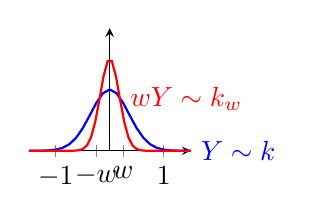
\begin{tikzpicture}
		\begin{axis}[
				width=0.3\textwidth,
				axis lines=middle,
				no markers,
				xtick={-2, -0.5, 0, 0.5, 2},
				ytick=\empty,
				xticklabels={$-1$, $-w$, {}, $w$, $1$},
				clip=false,
				xlabel={},
				ylabel={},
				domain=-3:3,
				ymin=0, ymax=2,
				xmin= -3, xmax=3,
				view = {0}{90}
			]
			\addplot[blue, thick] {exp(-x^2)} node[right] {$Y \sim k$};
			\addplot[red, thick, samples=40] {1.5*exp(-4*x^2)} node[pos=0.6, right] {$wY \sim k_w$};

		\end{axis}
	\end{tikzpicture}
\end{center}

Now, our goal is to find the optimal $w$ to approximate $Z(\sim \delta_0)$ by $Z + Y_w$.

Correspondingly, we approximate $f(x)$ by
\[\hat f(x) = \hat f_{n, w}(x, X_1, \dots, X_n) = \frac{1}{n} \sum_{i=1}^n k_w(x - X_i)\]

\begin{center}
	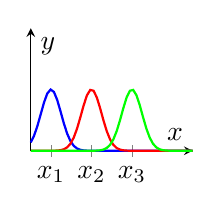
\begin{tikzpicture}
		\begin{axis}[
				width=0.3\textwidth,
				axis lines=middle,
				no markers,
				xtick={1, 3, 5},
				ytick=\empty,
				xticklabels={$x_1$, $x_2$, $x_3$},
				clip=false,
				xlabel={$x$},
				ylabel={$y$},
				domain=0:8,
				ymin=0, ymax=2,
				xmin=0, xmax=8,
				samples=50,
				view = {0}{90}
			]
			\addplot[blue, thick] {exp(-2*(x-1)^2)};
			\addplot[red, thick] {exp(-2*(x-3)^2)};
			\addplot[green, thick] {exp(-2*(x-5)^2)};
		\end{axis}
	\end{tikzpicture}
\end{center}

Our plan is to use $\MSE = \text{bias}^2 + \text{variance}$ as
\begin{center}
	\begin{tabular}{c|cc}
		$w\searrow 0$      & $\text{bias} \searrow$ & $\text{variance} \nearrow$ \\
		$w\nearrow \infty$ & $\text{bias} \nearrow$ & $\text{variance} \searrow$
	\end{tabular}
\end{center}

\tbf{Integrated Square Error (ISE):}
\[\ISE = \int_{\R} \abs{\hat f_n(x, X_1, \dots, X_n) - f(x)}^2\; dx\]

Since this is a random variable, we can also define \emph{mean integrated square error}.

\tbf{Mean Integrated Square ERROR (MISE):}
\begin{align*}
	\text{MISE} = \E[\ISE] & = \int_{\R} \E\abs{\hat f(x, X_1, \dots, X_n) - f(x)}^2\; dx                                                                                                     \\
	                       & = \int_{\R} \E\abs{\hat f(x, X_{1:n}) - \E[\hat f_n(x, X_{1:n})] + \E[\hat f_n(x, X_{1:n})]- f(x)}^2\; dx                                                        \\
	                       & =\int_{\R} \abs{\E \hat f_n(x, X_{1:n}) - f(x)}^2\; dx + \int_{\R} \E\abs{\hat f_n(x, X_{1:n}) - \E[\hat f_n(x, X_{1:n})]}^2\; dx                                \\
	                       & = \int_{\R} \underbrace{\abs{\E \hat f_n(x, X_{1:n}) - f(x)}^2}_{\text{bias}^2}\; dx + \int_{\R} \underbrace{\Var[\hat f_n(x, X_{1:n})]}_{\text{variation}}\; dx
\end{align*}

We can apply this formula to the kernel density estimator so we have bias:
\begin{align*}
	B_{n, w}(x) & = \E[\hat f_n(x, X_1, \dots, X_n)] - f(x)                         \\
	            & = \frac{1}{n} \sum_{i=1}^n \E[k_w(x - X_i)] - f(x)                \\
	            & = \frac{1}{n} \sum_{i=1}^n \int_{\R} f(t) k_w(x - t) \; dt - f(x) \\
	            & = \int_{\R} f(t) k_w(x - t) \; dt - f(x)
\end{align*}

\section{Feb 26}

\tbf{Recall:} For a continuous density $f$ with $X_1, \dots, X_n \iid f$, we would like to estimate $f$ but our normal method $\hat p_n = \frac{1}{n} \sum_{i=1}^n \delta_{X_i}$ is discrete, hence insufficient.

Hence, we introduce the \emph{Kernel Density Estimator}:
\[\hat f_{n, w}(x, X_1, \dots, X_n) = \frac{1}{n} \sum_{i=1}^n k_w(x - X_i)\]
where
\[k_w(t) = \frac{1}{w} k(\frac{t}{w}), \quad k \text{ some density}\]
is parameterized by the bandwidth $w$.

\tbf{Remark:} Above, we are using the Dirac Measure $\delta_x(A) = \begin{cases}
		1 & \text{if } x \in A \\
		0 & \text{otherwise}
	\end{cases}$ instead of the indicator function ($\ind: \R \to \R$) because we need a measure and not a function.

\tbf{Goal:} Find the ``optimal'' $w$.

We introduced the \emph{Integrated Square Error} (ISE), $\int_x \abs{\hat f(x) - f(x)}^2\; dx$ and the \emph{Mean Integrated Square Error} (MISE)
\[\text{MISE} = \E[\text{ISE}]= \int_x [(\text{bias}(x))^2 + \Var(x)]\; dx\]
where
\begin{align*}
	\text{bias(x)} & = \E[\hat f(x)] - f(x)                            \\
	\E[\hat f(x)]  & = \frac{1}{n} \sum_{i=1}^n \E_{X_i}[k_w(x - X_i)] \\
	               & = \E[k_w(x - X_1)] \qquad (X_i \iid f)            \\
	               & = \int_{\R} f(t) k_w(x - t)\; dt
\end{align*}

\tbf{Convolution:} Let $Z \sim f$ and $Y \sim g$ be independent. Then
\[Z + Y \sim (f \star g)(x) = \int_{\R} f(t)\; g(x - t)\; dt\]

Hence,
\[\E[\hat f(x)] = (f \star k_w)(x)\]
which means that $\E[\hat f]$ is the density of $Z + Y_w$ where $Z \perp Y_w$ and $Z \sim f$ and $Y_w \sim k_w$.

What does this tell us about the behavior?
\begin{itemize}
	\item For $Y \sim k$, $Y_w \sim wY$ so $\E[\hat f] \to f$ as $w \to 0$.
	\item As $w \to \infty$, our support becomes infinitely large so $\E[\hat f] \to 0$.
\end{itemize}

Hence,
\[(\text{bias}(x))^2 = (\E[\hat f(x)] - f(x))^2 = \begin{cases}
		0      & w\to 0      \\
		f^2(x) & w\to \infty
	\end{cases}\]

Now, let's calculate the variance term:

\begin{align*}
	\Var(x) & = \Var(\hat f(x))                                                                                              \\
	        & = \Var\left(\frac{1}{n} \sum_{i=1}^n k_w(x - X_i)\right)                                                       \\
	        & = \frac{1}{n^2} \sum \Var(k_w(x- X_i)) \qquad (\text{independence})                                            \\
	        & = \frac{1}{n}\Var(k_w(x - X_i)) \qquad (\text{identically distributed})                                        \\
	        & = \underbrace{\frac{1}{n}\E[(k_w(x- X_i))^2]}_{V^{(1)}} - \underbrace{\frac{1}{n}[\E[k_w(x-x_i)]]}_{V^{(2)}}^2
\end{align*}

From our previous work,
\[V^{(2)} = \frac{1}{n} \mathcal{I}^2 \to \begin{cases}
		\frac{1}{n} f^2(x) & w\to 0      \\
		0                  & w\to \infty
	\end{cases}\]
and
\begin{align*}
	V^{(1)} & = \frac{1}{n} \int f(g) k^2_w(x - t)\; dt                                           \\
	        & = \frac{1}{n} \frac{1}{w}\int f(t) \frac{1}{w} k^2\left(\frac{x - t}{w}\right)\; dt \\
	        & = \frac{1}{n} \frac{1}{w} \int f(ws + t) k^2(s)\; ds \qquad (s = \frac{x - t}{w})   \\
	        & \to \begin{cases}
		              \infty & w\to 0      \\
		              0      & w\to \infty
	              \end{cases}
\end{align*}
since the constant $\frac{1}{w}$ term dominates the bounded $f, k$.

\section{Feb 28}

\begin{proposition}
	\textbf{Theorem:} Assume $f$ and $k$ smooth. Then as $w \to 0$,
	\[\text{MISE}_{n, w} = \underbrace{\alpha w^4}_{\text{bias}} + \underbrace{\frac{\beta}{nw}}_{\text{variance}} + \text{error}\]
\end{proposition}

How do we choose $w$? Ignoring $\alpha, \beta$, it makes sense we want to minimize MISE:
\[(w^4 + \frac{1}{nw})' = 4w^3 - \frac{1}{nw^2} = 0 \implies w^5 \propto \frac{1}{n}  \implies w \propto n^{-1/5} \]

This is \tbf{Sylverman's Rule of Thumb:} up to unknown bias and variance, choose $w = n^{-1/5}$.

However, assuming we do not know $\alpha, \beta$, this is not a very good estimate -- it does not even depend on the density $f$! Can we do better?

Recall the setup: $X_1, X_2, \, \dots,\, X_n \iid f$ with estimator
\[\hat f_{n, w}(x) = \frac{1}{n} \sum_{i=1}^n k_w(x - X_i)\]

We want to find $w$. Last time, we looked at the MISE. This time, consider only the ISE. Our goal is to minimize:
\begin{align*}
	\text{ISE} & = \int_x \abs{\hat f_{n, w}(x) - f(x)}^2\; dx                     \\
	           & = \int \hat f_{n, w}(x) - 2\int \hat f \cdot f + \int f^2(x)\; dx
\end{align*}

Define
\begin{align*}
	I & = \int_x \hat f_{n, w}(x) \cdot f(x)\; dx                                                                               \\
	  & = \E_{X_{n+1} \sim f}[\hat f_{n, w}(X_{n+1})] \qquad (X_{1:n} \iid f)                                                   \\
	  & = \E[\hat f_{n, w}(X_{n+1}; X_1, \dots, X_n) ]                                                                          \\
	  & \approx \E[\hat f_{n-1, w}(X_{n}; X_1, \dots, X_{n-1})]                                                                 \\
	  & \approx \frac{1}{n} \sum_{i=1}^n \E[\hat f_{n- 1, w}(X_i; i^X)] \qquad (i^X = X_1, \dots, X_{i-1}, X_{i+1}, \dots, X_n) \\
	  & = \frac{1}{n} \sum_{i=1}^n \hat f_{n-1, w}^{(i)}(X_i)
\end{align*}

We call this the \tbf{cross-validation} (leave-one-out) estimator.

Since the last term does not depend on $w$, it suffices to find
\[\argmin_w \hat J(w) = \int \hat f_{n, w}(x)^2 - 2 \frac{1}{n} \sum_{i=1}^n \hat f_{n-1, w}^{(i)}(X_i)\]

And this is exactly what we want since this minimization problem depends only on the kernel and not on the distribution $f$.

\begin{proposition}
	\textbf{Theorem (Stone 1984):}
	\[\P\left(\lim_{n \to \infty} \frac{\ISE(\hat f_{\hat w_n}, f)}{\inf_w \ISE(\hat f_{w, n}, f)} = 1\right) = 1 \]
	(i.e. almost surely)
\end{proposition}

However, this convergence could be very slow (especially for $X_i \sim f \in \R^d, \; d \gg 1$)

\tbf{Example:} For $f$ Gaussian in $\R^d$ with $f(0) = \left(\frac{1}{\sqrt{2\pi}}\right)^d$, to have
\[\abs{\hat f_{\hat w_n} - f(0)} \leq \frac{1}{10} f(0)\]

\begin{center}
	\begin{tabular}{c|c}
		$d$ & $n$    \\ \hline
		1   & 4      \\
		2   & 19     \\
		5   & 768    \\
		10  & 842000 \\
		$\vdots$
	\end{tabular}
\end{center}

which is very fast growth

\section{March 3}
\subsection{Maximum Likelihood Estimation}

\tbf{Setup:} Sample $X_1,\, \dots,\, X_n \sim p_{\theta}$ with $\theta$ unknown. We want to find $\theta$ that makes $X_1 =x_1, \dots, X_n = x_n$ most likely (i.e. the parameter that defines the distribution that best fits the observation)

\begin{align*}
	\hat \theta & = \argmax_{\tilde \theta} p_{\tilde \theta}(X_1 = x_1, \dots, X_n = x_n)                                                        \\
	            & = \argmax_{\tilde \theta} p_{\tilde \theta}(x_1)\cdots p_{\tilde \theta}(x_n)                                                   \\
	            & = \argmax_{\tilde \theta} \frac{1}{n} \sum_{i=1}^n \log p_{\tilde \theta}(x_i)                                                  \\
	            & = \argmax_{\tilde \theta} \sum_{x=1}^s (\log p_{\tilde \theta}(x)) \hat p(x)                                                    \\
	            & = \argmin_{\tilde \theta} -\sum_{x=1}^{s} \hat p(x) \log p_{\tilde \theta}(x)                                                   \\
	            & = \argmin_{\tilde \theta} -\sum_{x=1}^{s} \hat p(x) \log \frac{\hat p(x)}{p_{\tilde \theta}(x)} - \sum \hat p(x) \log \hat p(x) \\
	            & = \argmin_{\tilde \theta} D(\hat p \parallel p_{\tilde \theta}) + H(\hat p)                                                     \\
	            & = \argmin_{\tilde \theta} D(\hat p \parallel p_{\tilde \theta})
\end{align*}
since the entropy term does not depend on $\theta$.

\tbf{Conclusion:} MLE is equivalent to finding the distribution that is closest in KL-divergence to the empirical distribution.

\tbf{Example:} $X_1, \dots, X_n \sim \Nc(\mu, 1)$. Equivalently, $f_{\mu} = \frac{1}{\sqrt{2\pi}} e^{-\frac{(x-\mu)^2}{2}}$.

Hence,
\begin{align*}
	\hat \mu & = \argmax_{\tilde \mu} \prod_{i=1}^n f_{\mu}(x_i)               \\
	         & = \argmax \exp\left(\sum -\frac{(x_i - \tilde \mu)^2}{2}\right) \\
	         & = \argmin \sum_{i=1}^n (x_i - \tilde \mu)^2                     \\
	         & \overset{*}{=} \frac{1}{n} \sum_{i=1}^n x_i
\end{align*}

\begin{exercise}
	\textbf{Exercise:} Prove the starred equality above.
\end{exercise}

\tbf{Example:} $X_1, \dots, X_n \sim f_{\lambda} = \frac{1}{Z_{\lambda}} p(x) \exp\left(\sum_{j=1}^c \lambda_j \Ec_j(x)\right) $

Then
\begin{align*}
	\hat \lambda & = \argmax \prod f_{\tilde \lambda} (x_i)                                                                                                                    \\
	             & = \argmin -\frac{1}{n} \sum_{i=1}^{n} \log(f_{\tilde \lambda}(x_i)) \qquad (\text{invariant under constant})                                                \\
	             & = \argmin -\frac{1}{n} \sum_{i=1}^{n} \log\left(\frac{1}{Z_{\lambda}} p(x_i) \exp\left(\sum_{j=1}^c \lambda_j \Ec_j(x)\right)\right)                        \\
	             & = \argmin -\frac{1}{n} \sum_{i=1}^{n} \log\left(\frac{1}{Z_{\lambda}} \exp\left(\sum_{j=1}^c \lambda_j \Ec_j(x)\right)\right) \qquad (p(x_i) \text{ known}) \\
	             & = \argmin \log(Z_{\tilde \lambda}) - \frac{1}{n} \sum_{i=1}^n \sum_{j=1}^{c} \tilde \lambda_j \Ec_j(x_i)                                                    \\
	             & = \argmin \log(Z_{\tilde \lambda}) - \sum_{j=1}^{c} \lambda_j \left(\frac{1}{n} \sum_{i=1}^n \Ec_j(x_i)\right)                                              \\
	             & = \argmin \log(Z_{\tilde \lambda}) - \sum_{j=1}^{c} \lambda_j \theta_j
\end{align*}
where $\theta_j = \frac{1}{n} \sum_{i=1}^n \Ec_j(x_i)$ are the observed statistics.

\subsection{Classification}

\tbf{Motivation:} Suppose we set up outside the dining hall and observe the patterns of the rush. There is a large group that comes in at noon and another group that comes in later

\begin{center}
	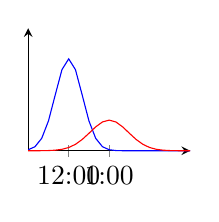
\begin{tikzpicture}
		\begin{axis}[
				width=0.3\textwidth,
				axis lines=middle,
				no markers,
				xtick={1.5, 3},
				xticklabels={12:00, 1:00},
				ytick=\empty,
				clip=false,
				xlabel={},
				ylabel={},
				domain=0:6,
				ymin=0, ymax=2,
				xmin=0, xmax=6,
				view = {0}{90}
			]
			\addplot[blue] {1.5*e^(-2*(x-1.5)^2)};
			\addplot[red] {0.5*e^(-(x-3)^2)};
		\end{axis}
	\end{tikzpicture}
\end{center}

If we interviewed a student at 2:00, it is quite likely they will be from group two. Similarly, if we interviewed a student at 10:00, they are likely from group one. But what about at 12:30? This is the problem of classification.

Formally, let $X \in \R^d$ be some random variable. Let $Y = \{1, \dots, c\}$ be classes with $\pi_i = \P(Y = i)$ and $f_i(x)$ the class conditioned density (in the example above, $f_2$ would be the red curve).

Then for any set $A$,
\[P_X(A) = \sum_{i=1}^{c} \pi_i \P(A)\]
and
\[f_X(A) = \sum_{i=1}^{c} \pi_i f_i(A)\]

We define a \tbf{classification} $h: \R^d \to \{1, \dots, c\}$.

\section{March 5}

\begin{proposition}
	\textbf{Bayes' Classification Rule:}
	\[h^*(x) = \argmax_{i =1:c} \P(Y = i \; | \; X = x) \]
\end{proposition}

\tbf{Example:} $Y \in \{1, 2\}$.
\begin{align*}
	\P(Y = 1\; | \; X = x) & = \frac{\P(Y= 1, X = x)}{\P(X = x)}               \\
	                       & = \frac{\P(Y=1) \P(X = x \; | \; Y= 1)}{\P(X= x)} \\
	                       & = \frac{\pi_1 \cdot f_1(x)}{\P(X = x)}            \\
	\P(Y = 2\; | \; X = x) & = \frac{\pi_2 \cdot f_2(x)}{\P(X = x)}
\end{align*}

Hence,
\[h^*(x) = \begin{cases}
		2 & \pi_1 f_1(x) < \pi_2 f_2(x) \\
		1 & \text{otherwise}
	\end{cases}\]

In what sense can we say $h^*$ is the ``best'' classifier?
\[\P(h^*(X) \neq Y) \leq \P(h(x) \neq Y) \qquad \forall h: \R^d \to \{1, \dots, c\}\]

\begin{exercise}
	\textbf{Exercise:} Prove the optimality of Bayes' classification rule. Hint:
	\[\P(h^*(X) = Y) = \int_x \P(Y = h^*(x) \; | \; X = x) f_X(x)\; dx\]

	\div

	\emph{Proof:}
	\begin{align*}
		\P(h^*(x) \neq Y) & = 1 - \P(h^*(x) = Y)                                                             \\
		                  & = 1 - \int_x \P(Y = h^*(x) \; | \; X = x) f_X(x)\; dx                            \\
		                  & = 1 - \int_x \P(Y = \argmax_i [\P(Y = i \; | \; X = x)]; | \; X = x) f_X(x)\; dx \\
		                  & \leq 1 - \int_X \P(Y = h(x) \; | \;X = x) f_X(x)\; dx                            \\
		                  & = 1 - \P(h(X) = Y)                                                               \\
		                  & = \P(h(X) \neq Y)
	\end{align*}
\end{exercise}


In applications, however, we may be able to approximate the $f_i$'s by sampling but not necessarily the $\pi_i$'s.

\begin{proposition}
	\textbf{Neyman-Pearson (NP) Classification:} Fix $t \in (0, \infty)$. Then
	\[h_t(x) = \begin{cases}
			1 & \text{if } \frac{f_2(x)}{f_1(x)} < t \\
			2 & \text{if } \frac{f_2(x)}{f_1(x)} > t \\
		\end{cases}\]
\end{proposition}

\tbf{Remark:} In the case $t = \frac{\pi_1}{\pi_2}$, then NP is equivalent to Bayes.

If $Y = 1$ represents a negative test and $Y = 2$ represents a positive test, we have
\begin{itemize}
	\item The detection rate $\P(h(X) = 2 \; | \; Y = 2)$
	\item The false alarm rate $\P(h(X) = 2 \; | \; Y = 1)$
\end{itemize}

Intuitively, we would like to maximize the detection rate while minimizing the false alarm rate.

\begin{tbox}{\textbf{Theorem:} Fix $t \in (0, \infty)$. Let $h$ be any other classifier. If $\text{FAR}_h \leq \text{FAR}_{h_t}$, then $\text{DR}_h \leq \text{DR}_{h_t}$}
	\emph{Intuition:}

	We have
	\[\text{FAR}_{h_t} = \P(h(X) = 2 \; | \; Y = 1) = \P(\frac{f_2(x)}{f_1(x)} > t \; | \; Y= 1)\]
	so as $t \to \infty$, $\text{FAR}_{h_t} \searrow$ and $\text{DR}_t \searrow$

	Under NP classification,
	\begin{center}
		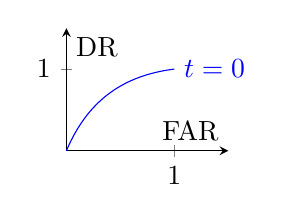
\begin{tikzpicture}
			\begin{axis}[
					width=0.3\textwidth,
					axis lines=middle,
					no markers,
					xtick={1},
					ytick={1},
					clip=false,
					xlabel={FAR},
					ylabel={DR},
					domain=-2:2,
					ymin=0, ymax=1.5,
					xmin=0, xmax=1.5,
					view = {0}{90}
				]
				\draw[blue] (0, 0) to[bend left] (1, 1) node[right] {$t = 0$};
			\end{axis}
		\end{tikzpicture}
	\end{center}

	\div

	\emph{Proof:}

	\begin{center}
		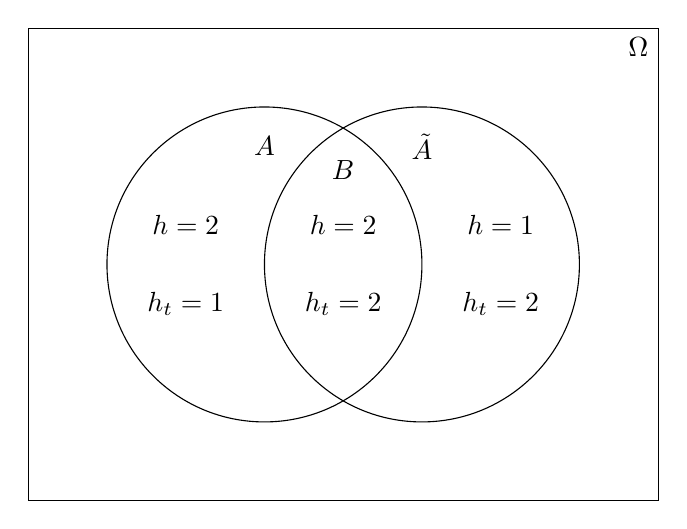
\begin{tikzpicture}

			\draw (-3, -3) rectangle (5, 3) node[below left] {$\Omega$};

			\draw (0, 0) circle (2);
			\draw (2, 0) circle (2);

			\node at (0, 1.5) {\tbf{$A$}};
			\node at (2, 1.5) {\tbf{$\tilde A$}};
			\node at (1, 1.2) {\tbf{$B$}};

			\node at (-1, 0.5) {$h = 2$};
			\node at (-1, -0.5) {$h_t = 1$};

			\node at (3, 0.5) {$h = 1$};
			\node at (3, -0.5) {$h_t = 2$};

			\node at (1, 0.5) {$h = 2$};
			\node at (1, -0.5) {$h_t = 2$};
		\end{tikzpicture}
	\end{center}

	We have
	\begin{align*}
		\text{FAR}_h & = \P(h(X) = 2 \; | \; Y=1)   \\
		             & = \P(A \cup B \; | \; Y = 1) \\
		             & = p_1(A \cup B)
	\end{align*}
	where $p_1$ is the marginal conditioned on the class being $1$.

	Then:
	\begin{enumerate}
		\item $p_1(A \cup B) \leq p_1(\tilde A \cup B) \implies p_1(A) \leq p_1(\tilde A)$ (since $A, B$ disjoint).

		      We want to show $p_{\alpha}(A) \leq p_2(\tilde A)$

		      Notice
		      \begin{align*}
			      A        & \sub \{h_t(x) = 1\} = \left\{\frac{f_2(x)}{f_1(x)} < t\right\} = \{f_2(X) < t \cdot f_1(X)\} \\
			      \tilde A & \sub \{h_t(x) = 2\} = \left\{\frac{f_2(x)}{f_1(x)} > t\right\} = \{f_2(X) > t \cdot f_1(X)\} \\
		      \end{align*}

		      We have
		      \begin{align*}
			      p_1(X \in A)                         & \leq p_1(X\in \tilde A)             \\
			      p_1(X \in A) = t \int_A f_1(X)\; d\P & \leq t \int_{\tilde A} f_1(X)\; d\P
		      \end{align*}
	\end{enumerate}
\end{tbox}

\section{March 7}

\tbf{Motivation:} for training data $(X_1, Y_1) \dots (X_n, Y_n)$ with $X_i \in \R^d$ and $Y_i \in \{1, \dots, s\}$, we would like to build $h: \R^d \to \{1, \dots, s\}$.

There are multiple different approaces:
\begin{itemize}
	\item Generative
	\item Discriminative
	\item Algorithmic
\end{itemize}

\subsection{Generative Classifiers}
\[h^*(x) = \argmax_{x \in \{1, \dots, s\}} \P(Y = c \; | \; X = x) = \argmax_c \frac{\pi_c f_c(x)}{\P(X = x)}\]

A good estimator given data $(X_1, Y_1) \dots (X_n, Y_n)$ is clearly
\[\hat \pi_c = \frac{\#\{i: Y_i = c\}}{n}\]

But what if we do not know $f_c$? This gets especially difficult when $d$ is large.

\tbf{Naive Bayes:} Assume $X = (X^1, X^2, \dots, X^d)$ and $f_c(x^1, \dots, x^d) = f_c^1(x^1) \cdots f_c^d(x^d)$.

Then instead of needing to find $(f_c)^s$ with $f_c: \R^d \to \R$, it suffices to find $(f_c^k)_{k=1:d}^{c=1:s}$ for $f_c^k: \R \to \R$

\tbf{Quadratic Discriminant Analysis (QDA):}
Assume
\[f_c(x) \sim \Nc(\mu_c, \Sigma_c)\]

Then
\[f_c(x, \mu_c, \Sigma_c) = \frac{1}{\sqrt{(2\pi)^d \abs{\Sigma}}} \exp(-\frac{1}{2} (x - \mu_c)^T \Sigma_c^{-1}(x - \mu))\]
for $x \in \R^{d \times 1}$, $\mu_c \in \R^{d \times 1}$, $\Sigma_c \in \R^{d\times d}$

However, if we are to attempt MLE on $\mu_c, \Sigma_c$, we need to ensure that we have enough data $n$ to estimate the $d^2s$ parameters across classes $\{1, \dots, s\}$. In practice, this can lead to over fitting.

\section{March 10}

\tbf{Definition:} If we partition a space $\Omega = \bigcup_{i=1}^s A_i$ into disjoint sets, then \emph{precision boundary} of $A_i$ is $\partial A_i = A_i \setminus \overset{\circ}{A}_i$.

Last time, we saw a classification method that let us use the MLE on high-dimensional spaces but which required a lot of data in practice. This was the Quadratic Discriminant Analysis (QDA), which had a quadratic precision boundary.

\begin{center}
	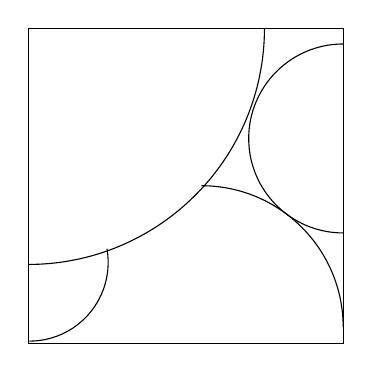
\begin{tikzpicture}
		\draw (0, 0) rectangle (4, 4);
		\draw (3, 4) arc (0:-90:3);
		\draw (1, 1.2) arc (10:-90:1);
		\draw (2.2, 2) arc (90:0:1.8);
		\draw (4, 3.8) arc (90:270:1.2);




	\end{tikzpicture}
\end{center}

We can follow a similar but slightly less flexible approach.

\tbf{Linear Discriminant Analysis:}

Assume $f_c \sim \Nc(\mu_c, \Sigma)$.

Then the precision boundary is given by
\[\left\{x \in \R^d: \frac{f_2(x)}{f_1(t)} = t\right\}\]
from NP. We claim this is a linear set.

\begin{proof}
	\emph{Proof:} By assumption, $f_1 \sim \Nc(\mu_1, \Sigma)$ where $\mu_1 \in \R^d$ and $\Sigma \in \R^{d \times d}$.

	Then
	\[f_1(x) = \frac{1}{(2\pi)^{d/2} \abs{\Sigma}^{d/2}} \exp\left(-\frac{1}{2} (x- \mu_1)^T \Sigma^{-1}(x-\mu_1)\right) \]
	notice
	\[(x- \mu_1)^T \Sigma^{-1}(x-\mu) \in \R^{(1 \times d)(d \times d)(d \times 1)} = \R^1\]

	Similarly, we can write
	\[f_2(x) = \frac{1}{(2\pi)^{d/2} \abs{\Sigma}^{d/2}} \exp\left(-\frac{1}{2} (x- \mu_2)^T \Sigma^{-1}(x-\mu_2)\right) \]
	so
	\[\log t = \log \frac{f_1}{f_2} = \frac{1}{2} (x- \mu_1)^T \Sigma^{-1} (x - \mu_1) - (x - \mu_2)^T \Sigma^{-1} (x - \mu_2)\]

	In the case $d=1$, we have $\Sigma = \sigma^2$ so
	\[\log t = \frac{(x- \mu_1)^2}{\sigma^2} - \frac{(x - \mu_2)^2}{\sigma^2} = -\frac{2x(\mu_1 - \mu_2) + \mu_1^2 + \mu_2^2}{\sigma^2}\]
	but in the QDA case, we would have $\Sigma = (\sigma^2_1, \sigma^2_2)$ so the terms would not cancel.
\end{proof}

\subsection{Discriminative Construction}
Recall that in the Bayes' classification rule (the optimal case),
\[h^*(x) = \argmax_{c \in \{1, \dots, s\}} \P(Y = c \; | \; X = x)\]

Earlier, we wrote $\P(Y = c \; | \; X= x) = \pi_c f_c(x)$ and tried to estimate $\pi_c$ and $f_c$. But what if we tried to estimate $r_c(x) = \P(Y = c \; | \; X = x)$ directly?

\tbf{Linear Regression:} For $s= 2$, we want $r_1(x)$ and $r_2(x)$ satisfying $r_1(x) + r_2(x) = 1$. It seems reasonable to try linear regression.

We can model
\begin{gather*}
	\log \frac{r_2(x)}{r_1(x)} = \alpha + \beta x\\
	\log \frac{r_2}{1-r_2} = \alpha + \beta x\\
	r_2 = \frac{e^{\alpha + \beta x}}{1 + e^{\alpha + \beta x}}
\end{gather*}

\tbf{Softmax:} Softmax is a generalization of logistic regression for $s > 2$.

As before,
\[\log \frac{r_k(x)}{r_1(x)} = \alpha_k + \beta_k x \implies r_k(x) = \frac{e^{\alpha_k + \beta_k x}}{1 + \sum_{k=n}^s e^{\alpha_k + \beta_k x} }\]

Then we can use MLE to estimate $\alpha_k, \beta_k$.

\section{March 14}
\subsection{Discriminative Classification Continued}
\tbf{k-Nearest Neighbor Classification:}

Let $D_k(x)$ be the closed ball centered at $x$ with radius $R_k(x)$, the smallest radius that contains $k$ data points.

\begin{center}
	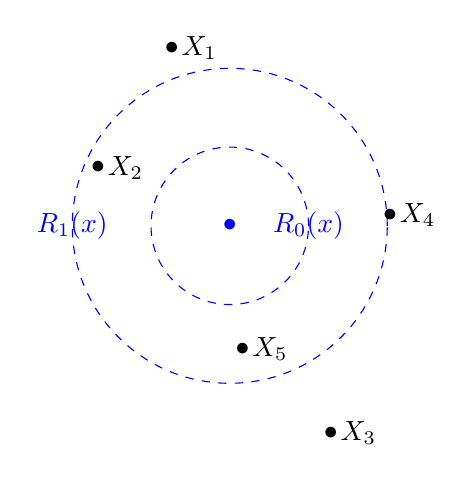
\begin{tikzpicture}
		\node[blue] at (0,0) {$\bullet$};
		\draw[blue, dashed] (0, 0) circle (1);
		\draw[blue, dashed] (0, 0) circle (2);

		\node[blue] at (1, 0) {$R_0(x)$};
		\node[blue] at (-2, 0) {$R_1(x)$};

		\foreach \x in {1, ..., 5} {
				\node (p-\x) at (rand*3, rand*3) {$\bullet$};
				\node[right] at (p-\x) {$X_{\x}$};
			}
	\end{tikzpicture}
\end{center}

If we fix $k$, as $n \to \infty$, $R_k(x) \to 0$ which gives us the estimator
\[\hat r_c(x) = \frac{\#\{i: X_i \in B(x, R_k(x)),\; Y_i = c\}}{k}\]

\begin{tbox}{\textbf{Claim:} $\hat r_c(x) \to r_c(x)$, i.e. the K-NN estimator is consistent }
	\emph{Proof:}

	\begin{align*}
		\hat r_c(x) & = \frac{\#\{i: X_i \in B(x, R_k(x)), Y_i = c\}}{\#\{i: X_i \in B(c, R_k(x))\}}                     \\
		            & = \frac{\#\{i: X_i \in B(x, \ep), Y_i = c\}/n}{\#\{i: X_i \in B(c, \ep)\}/n} \qquad (\ep = R_k(x)) \\
		            & \overset{n\to\infty}{\longrightarrow} \frac{\P(X \in B(x, \ep),\; Y=c)}{\P(X \in B(x, \ep))}       \\
		            & \overset{*}{=} \frac{\P(Y = c) \P(X \in B(x, \ep) \; | \; Y=c)}{\P(X \in B(x, \ep))}               \\
		            & = \P(Y = c) \frac{\int_{B(x, \ep)} f_c(t)\; dt}{\int_{B(x, \ep)} f(t)\; dt}                        \\
		            & \approx \P(Y = c) \frac{f_c(x) \abs{B(x, \ep)}}{f(x) \abs{B(x, \ep)}}                              \\
		            & = \P(Y = c) \frac{f_c(x)}{f(x)}                                                                    \\
		            & = \frac{\P(Y = c) \P(X = x \; | \; Y=c)}{P(X = x)}                                                 \\
		            & = \frac{\P(X = x, \; Y = c)}{\P(X = x)}                                                            \\
		            & = \P(Y = c \; | \; X = x)                                                                          \\
		            & = r_c(x)
	\end{align*}

	\tbf{Remark:} This is not entirely rigorous since we are taking both $n \to \infty$ and $\ep \to 0$. It would not be too difficult to make this rigorous by estimating the error of the limit $n \to \infty$. Leaving the way open to rigor is also why we cannot say
	\[\frac{\P(Y = c) \P(X \in B(x, \ep) \; | \; Y=c)}{\P(X \in B(x, \ep))} = \P(Y = c \; | \; X \in B(x, \ep)) \overset{\ep \to 0}{\longrightarrow} \P(Y =c \; | \; X= x) = r_c(x)\]
	in the starred equality.
\end{tbox}

\tbf{Support Vector Machine:}
\[h^*(x) = \argmax_c r_c(x)\]

\emph{Example:} In the case $s=2$, we want $r_1, r_2$ which gives
\[h(x) = \frac{r_2(x)}{r_1(x)}\]
so it suffices to find the precision boundary

\begin{center}
	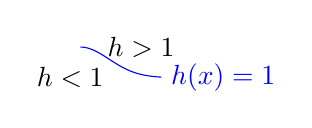
\begin{tikzpicture}
		\begin{axis}[
				width=0.3\textwidth,
				axis lines=middle,
				no markers,
				xtick=\empty,
				ytick=\empty,
				clip=false,
				xlabel={$x$},
				ylabel={$y$},
				domain=-2:2,
				ymin=-2, ymax=2,
				xmin= -2, xmax=2,
				view = {0}{90},
				hide x axis,
				hide y axis
			]
			\addplot[blue, domain=0:2] {exp(-x^2)} node[right] {$h(x) = 1$};
			\node at (1.5, 1) {$h > 1$};
			\node at (-0.25, 0) {$h < 1$};
		\end{axis}
	\end{tikzpicture}
\end{center}

The trick here is to find a transformation $\phi$ so that the precision boundary is linear

\begin{center}
	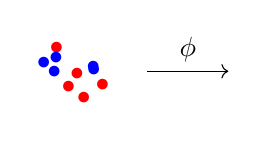
\begin{tikzpicture}
		\begin{axis}[
				width=0.3\textwidth,
				axis lines=middle,
				no markers,
				xtick=\empty,
				ytick=\empty,
				clip=false,
				xlabel={$x$},
				ylabel={$y$},
				domain=-2:2,
				ymin=-2, ymax=2,
				xmin= -2, xmax=2,
				view = {0}{90},
				hide x axis,
				hide y axis
			]

			\pgfplotsinvokeforeach{0, 1, 2, 3, 4} {
				\node[red] at (rand, rand+2) {$\bullet$};
				\node[blue] at (rand, rand+2) {$\bullet$};
			}

			\draw[->] (2, 2) -- (4, 2) node[midway, above] {$\phi$};
		\end{axis}
	\end{tikzpicture}
	\hspace{1cm}
	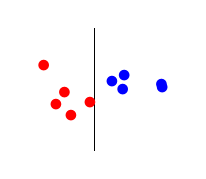
\begin{tikzpicture}
		\begin{axis}[
				width=0.3\textwidth,
				axis lines=middle,
				no markers,
				xtick=\empty,
				ytick=\empty,
				clip=false,
				xlabel={$x$},
				ylabel={$y$},
				domain=-2:2,
				ymin=-2, ymax=2,
				xmin= -2, xmax=2,
				view = {0}{90},
				hide x axis,
				hide y axis
			]
			\draw (0, -2) -- (0, 2);

			\pgfplotsinvokeforeach{0, 1, 2, 3, 4} {
				\node[red] at (rand-1, rand) {$\bullet$};
				\node[blue] at (rand+1, rand) {$\bullet$};
			}
		\end{axis}
	\end{tikzpicture}
\end{center}

\begin{exercise}
	\textbf{Bonus 3/14:} What is the setup for the classification problem? What does it mean to build a classifier?

	\div

	\tbf{Answer:} Given a set of data $\{(X_i, Y_i)\}_{i=1}^n$ on classes $Y_i \in \{1, \dots, s\}$ following an unknown distribution $f_c$ for $c \in \{1, \dots, s\}$, we want to find a function $h: \R^d \to \{1, \dots, s\}$ that best approximates the true distribution.

	Bayes' Rule suggests that the optimal behavior is
	\[h^*(x) = \argmax_c \P(Y = c \; | \; Y = x)\]

	Everything else is finding different ways to estimate this function.
\end{exercise}

\section{March 17}
\subsection{Support Vector Machine}

Given data $(X_1, Y_1), \dots, (X_n, Y_n)$, we want to find a function $h: \R^d \to \{1, \dots, s\}$ that best approximates the true distribution.

In $\R^d$, there exists a curve that partitions the data into regions where $h(x) = c$ for some $c \in \{1, \dots, s\}$. We want to find this curve. The idea behind support vector machines is to apply a transformation $\phi$ such that it suffices to choose a hyperplane (rather than a curve) in $\R^{d'}$ with $d' \gg d$.

\emph{Example ($d=1$):}

\begin{center}
	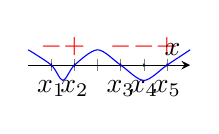
\begin{tikzpicture}
		\begin{axis}[
				width=0.3\textwidth,
				axis lines=middle,
				no markers,
				xtick={1, 2, 3, 4, 5, 6},
				ytick=\empty,
				xticklabels={$x_1$, $x_2$, , $x_3$, $x_4$, $x_5$},
				clip=false,
				xlabel={$x$},
				ylabel={$y$},
				domain=-2:2,
				ymin=-1, ymax=1,
				xmin=0, xmax=7,
				view = {0}{90},
				hide y axis
			]

			\draw[black] (1, 0) circle (0.01) node[above, red] {$-$};
			\draw[black] (2, 0) circle (0.01) node[above, red] {$+$};
			\draw[black] (4, 0) circle (0.01) node[above, red] {$-$};
			\draw[black] (5, 0) circle (0.01) node[above, red] {$-$};
			\draw[black] (6, 0) circle (0.01) node[above, red] {$+$};

			\addplot[smooth,blue] coordinates {
					(0, 0.25)
					(1, 0)
					(1.5, -0.25)
					(2, 0)
					(3, 0.25)
					(4, 0)
					(5, -0.25)
					(6, 0)
					(7, 0.25)
				};
		\end{axis}
	\end{tikzpicture}
\end{center}
with classifier
\begin{align*}
	h(x) & = \text{sign}((x - X_1)(x - X_2)(x-X_3)(x-X_5))                                    \\
	     & =  \text{sign}(\alpha_4 x^4 + \alpha_3 x^3 + \alpha_2 x^2 + \alpha_1 x + \alpha_0)
\end{align*}
so for $\phi: \R \to \R^5$ by $x \mapsto (1, x, x^2, x^3, x^4)$, we have
\[h(x) = \text{sign}(\vec a \cdot \phi(x))\]

However this presents a few problems: it depends on raising the dimension (something we are always looking to avoid), can lead to overfitting, and presents ambiguities -- if there are multiple such hyperplanes, which do we choose?

We will spend some time on this last question.

Consider the case

\begin{center}
	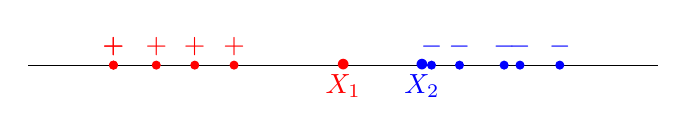
\begin{tikzpicture}

		\draw (-2, 0) -- (6, 0);

		\node[red] at (2, 0) {$\bullet$};
		\node[red, below] at (2, 0) {$X_1$};
		\node[blue] at (3, 0) {$\bullet$};
		\node[blue, below] at (3, 0) {$X_2$};

		\foreach \x in {0, ..., 4} {
				\draw[fill, red] (rand, 0) circle (0.05) node[above] {$+$};
				\draw[fill, blue] (rand+4, 0) circle (0.05) node[above] {$-$};
			}
	\end{tikzpicture}
\end{center}

Intuitively, we would like our classifier not to be too close to the data points nor to favor one class over the other.

In this case, $\frac{X_1 + X_2}{2}$ is a good choice which would give us classifier $h(x) = \text{sign}(\frac{X_1 + X_2}{2} - x)$.

In the general case, we would like to find the hyperplane that \emph{maximizes the minimal distance to the precision boundary.} We call the points closest to the hyperplane the \emph{support vectors} (in our example, $X_1, X_2$)

Formally, we want to find the hyperplane $0 = \alpha + \vec \beta \cdot x$ for $\alpha \in \R$, $\vec \beta, x \in \R^d$ which maximizes the minimal distance to the support vectors, yielding classifier
\[h(x) = \begin{cases}
		+ & \text{ if } \alpha + \beta x > 0 \\
		- & \text{ if } \alpha + \beta x < 0
	\end{cases} = \text{sign}(\alpha + \beta x)\]
following the convention that the normal vector $\beta$ is always chosen in the direction of the positive class.

What is the distance between a point $x \in \R^d$ to the hyperplane $\alpha + \beta x = 0$? Precisely $\norm{\alpha + \beta x}$.

Hence, the task moving forward is to find
\[(\alpha, \beta) = \argmax \left(\min_{i=1:n} \abs{\alpha + \beta x_i}\right) \]

\section{March 19}
\tbf{Recall:} We were looking for \emph{maximum margin classifiers} for Support Vector Machines: On data $(X_1, Y_1), \dots, (X_n, Y_n)$, find
\[(\hat \alpha, \hat \beta) = \argmax_{\alpha, \beta} \min_{i=1:n} \text{dist}(X_i, \{\alpha + \beta x =0 \})\]
for all $i: (\alpha + \beta X_i) Y_i \geq 0$.

Notice, the condition $(\alpha + \beta X_i) Y_i \geq 0$ is equivalent to the condition that the data is separable by the hyperplane $\alpha + \beta x = 0$.

Equivalently,
\[(\hat \alpha, \hat \beta) = \argmax_{\begin{subarray}{c}
			\alpha, \beta \\
			\norm{\beta} = 1\\
			\forall i: (\alpha + \beta X_i) Y_i \geq 0
		\end{subarray}} \min_{i=1:n} (\alpha + \beta X_i) Y_i = \argmax_{\alpha, \beta, \norm{\beta}=1} M\]
subject to $Y_i(\alpha + \beta X_i) \geq M$ for all $M$ since
\[\min \{a_1, \dots, a_n\} = \max M \quad a_i \geq M\; \forall M\]

Is this a convex optimazation problem, i.e are we optimizing a convex function on a convex set?

Already we run into difficulty with the condition $\norm B = 1$ since

\begin{center}
	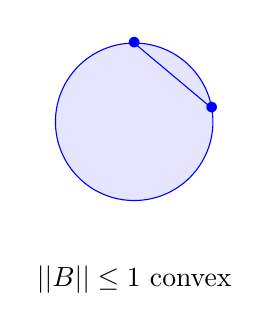
\begin{tikzpicture}

		\draw[blue, fill, fill opacity=0.1] (0, 0) circle (1);

		\draw[blue]  (90:1) -- (10:1);
		\node[blue] at (90:1) {$\bullet$};
		\node[blue] at (10:1) {$\bullet$};

		\node at (0, -2) {$\norm B \leq 1$ convex};
	\end{tikzpicture}\hspace{1cm}
	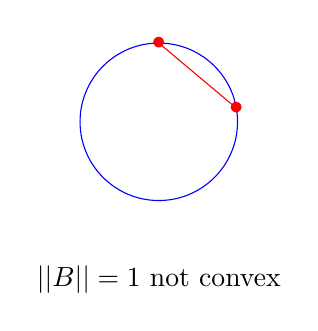
\begin{tikzpicture}

		\draw[blue] (0, 0) circle (1);

		\draw[red]  (90:1) -- (10:1);
		\node[red] at (90:1) {$\bullet$};
		\node[red] at (10:1) {$\bullet$};

		\node at (0, -2) {$\norm B = 1$ not convex};
	\end{tikzpicture}
\end{center}

Hence, we would like to reformulate the problem to remove the constraint $\norm B = 1$.

Consider the adjusted constraint $Y_i(\tilde \alpha, \tilde \beta) = Y_i(\frac{\alpha}{M} + \frac{\beta}{M} X_i) \geq 1$ for all $i$. T

Now
\[\norm{\tilde B} = \sum_{i=1}^{d} \tilde \beta_i^2 = \frac{1}{M^2}\]
so we can write
\[(\tilde \alpha, \tilde \beta) = \argmax_{\tilde \alpha, \tilde \beta} \frac{1}{\sum_{i=1}^{d} \tilde \beta_i^2 } = \argmin_{\tilde \alpha, \tilde \beta} \sum_{i=1}^{d} \tilde \beta_i^2 \]
subject to $Y_i(\tilde \alpha + \tilde \beta X_i) \geq 1\quad \forall i$

And indeed this is a convex optimization problem since $(\alpha, \beta) \mapsto \sum_{i=1}^d \beta_i^2$ is convex and the domain $B= \{(a, b): Y_i(a + b X_i) \geq 1\}$ is convex

\begin{proof}
	\emph{Proof:} Pick $(\alpha, \beta) \in B$ and $(\alpha', \beta') \in B$. Then for all $\lambda \in (0, 1)$,
	\[(\lambda a + (1-\lambda)a', \lambda \beta + (1- \lambda)\beta') \in B\]
	since by assumption,
	\begin{align*}
		(\alpha, \beta) \in B \implies Y_i(\alpha + \beta X_i) \geq 1     & \implies \lambda Y_i(\alpha + \beta X_i) \geq \lambda         \\
		(\alpha', \beta') \in B \implies Y_i(\alpha' + \beta' X_i) \geq 1 & \implies (1-\lambda) Y_i(\alpha' + \beta' X_i) \geq 1-\lambda
	\end{align*}
	\[\begin{array}{rl}
			\lambda Y_i(\alpha + \beta X_i) \geq \lambda         \\
			(1-\lambda) Y_i(\alpha' + \beta' X_i) \geq 1-\lambda \\ \hline
			\lambda Y_i(\alpha + \beta X_i) + (1-\lambda) Y_i(\alpha' + \beta' X_i) \geq 1
		\end{array}\]
	so indeed,
	\[Y_i(\alpha'' + \beta'' X_i) \geq 1\]
\end{proof}

Recall in the past to solve $\hat \theta = \argmin f(\theta)$ subject to $g(\theta) = 0$, we have used Lagrange multipliers:
\[\argmin f(\theta) + \lambda g(\theta)\]

For convex optimization problems, we introduce the \tbf{Lagrange Dual}:
\begin{enumerate}
	\item Find $\lambda = (\lambda_1, \dots, \lambda_n)$ subject to $\lambda_i \geq 0$
	\item Find $\hat \alpha = \hat \alpha(\lambda),\; \hat \beta = \hat \beta(\lambda)$ that minimize
	      \[\frac{1}{2}\sum_{j=1}^d \hat \beta_j^2 + \sum_{i=1}^n \lambda (1 - Y_i(\alpha + \beta X_i)) \tag{$\star$}\]
	\item Maximize ($\star$) over $\lambda$ to get $\hat \alpha, \beta$
\end{enumerate}

\chapter{Graphical Models}
\section{March 31}
\subsection{Gibbs Random Fields}

\tbf{Definition:} Let $G = (V, E)$ be a graph. Then we say a subset $C \sub V$ is a \emph{clique} if $\forall i \neq j \in C$, $(i, j) \in E$.

\emph{Example:} Let $G_1$ be given by
\begin{center}
	\begin{tikzpicture}[>= stealth, shorten >=2pt, line width =0.5 pt,
			node distance=2 cm]
		\node  at (0, 0) (one) {$ 1 $};
		\node [right of=one] (two) {$ 2 $};
		\node [below of=two] (three) {$ 3 $};

		\draw (one) -- (two) -- (three);
	\end{tikzpicture}
\end{center}

Then the cliques are $C_i = \{i\}$, $C_{12} = \{1, 2\}$, $C_{23} = \{2, 3\}$ but $C_{123} = \{1,2, 3\}$ is not a clique.

\tbf{Definition:} A \emph{Gibbs random field (GRF)} on a graph $G$ is a set of random variables $\{X_v\}_{v \in V}$ with the distribution
\[p(x) = \frac{1}{Z} \prod_{C \text{ sums over cliques in } G} \phi_c(x_c)\]
for some function $\phi_c: \Omega_c \to  [0, \infty)$ clique functions and $Z$ a partition function.

\tbf{Example:}

\begin{center}
	\begin{tikzpicture}[>= stealth, shorten >=2pt, line width =0.5 pt,
			node distance=2 cm]
		\node (one) at (0, 0) {$ 1 $};
		\node[below right of=one] (two) {$ 2 $};
		\node[above right of=one] (three) {$ 3 $};
		\node[right of=three] (four) {$ 4 $};

		\draw (one) -- (two) -- (three) -- (one);
		\draw (three) -- (four);
	\end{tikzpicture}
\end{center}

So for $C = \{1, 2, 3\}$ we have $X_C = (X_1, X_2, X_3)$ while for $C' = \{1, 2\}$ we have $X_{C'} = (X_1, X_2)$.

Hence $(X_1, \dots, X_4)$ is a GRF on $G$ if
\[p(x_1, x_2, x_3, x_4) = \frac{1}{Z} \phi_1(x_1) \phi_2(x_2) \phi_3(x_3) \phi_{12}(x_1, x_2) \phi_{13}(x_1, x_3) \phi_{23}(x_2, x_3) \phi_{34}(x_3, x_4) \phi_{123}(x_1, x_2, x_3)\]

\tbf{Example:} Let
\begin{itemize}
	\item $X_1 \sim \text{Bernoulli}(1/2)$
	\item $X_2 \sim \text{Bernoulli}(1/2), \; X_2 \perp X_1$
	\item $X_3 = X_1 \oplus X_2 = \begin{cases}
			      0 & X_1 = X_2    \\
			      1 & X_1 \neq X_2
		      \end{cases}$
	\item $X_4 = 1 - X_3$
\end{itemize}

\[p(1, 0, 1, 0) = p(X_1 =1, X_2 = 0, X_3 = 1, X_4 = 0) = p(X_1= 1, X_2 = 0) = \frac{1}{2} \cdot \frac{1}{2} = \frac{1}{4}\]
and
\[p(1, 0, 0, 0) = 0\]

What graph does this respect?
\[p(x_1, x_2, x_3, x_4) = \frac{1}{2} \cdot \frac{1}{2} \cdot \ind_{x_3 = x_1 \oplus x_2} \cdot \ind_{x_4 = 1 - x_3} = \frac{1}{Z} \phi_{123}(x_1, x_2, x_3) \phi_{34}(x_3, x_4)\]

Hence this is a GRF with respect to any graph that contains
\begin{center}
	\begin{tikzpicture}[>= stealth, shorten >=2pt, line width =0.5 pt,
			node distance=2 cm]
		\node (one) at (0, 0) {$ 1 $};
		\node[below right of=one] (two) {$ 2 $};
		\node[above right of=one] (three) {$ 3 $};
		\node[right of=three] (four) {$ 4 $};

		\draw (one) -- (two);
		\draw (one) -- (three);
		\draw (two) -- (three);
		\draw (three) -- (four);
	\end{tikzpicture}
\end{center}

For example:
\begin{center}
	\begin{tikzpicture}[>= stealth, shorten >=2pt, line width =0.5 pt,
			node distance=2 cm]
		\node (one) at (0, 0) {$ 1 $};
		\node[below right of=one] (two) {$ 2 $};
		\node[above right of=one] (three) {$ 3 $};
		\node[right of=three] (four) {$ 4 $};

		\draw (one) -- (two);
		\draw (one) -- (three);
		\draw (two) -- (three);
		\draw (three) -- (four);
		\draw (two) -- (four);
		\node[green!60!teal, node distance=1cm, below of=two] {$\checkmark$};
	\end{tikzpicture}
	\hspace{1cm}
	\begin{tikzpicture}[>= stealth, shorten >=2pt, line width =0.5 pt,
			node distance=2 cm]
		\node (one) at (0, 0) {$ 1 $};
		\node[below right of=one] (two) {$ 2 $};
		\node[above right of=one] (three) {$ 3 $};
		\node[right of=three] (four) {$ 4 $};

		\draw (one) -- (three);
		\draw (two) -- (three);
		\draw (three) -- (four);
		\node[red, node distance=1cm, below of=two] {$\times$};
	\end{tikzpicture}
\end{center}

What would a GRF on the second graph look like?

We know we must have a density of the form
\[p(x_1, x_2, x_3, x_4) = \frac{1}{Z}\phi_1(x_1) \cdots \phi_4(x_4) \phi_{13}(x_1, x_3) \phi_{23}(x_2, x_3)\phi_{34}(x_3, x_4)\]
but we cannot find functions $\phi_{13}(x_1, x_3) \phi_{23}(x_2, x_3)$.


\tbf{Remark:} Neither the representation $p(x) = \frac{1}{Z} \prod_{C \text{ sums over cliques}} \phi_c(x_c)$ nor the graph representing a particular distribution must not be unique.

\emph{Example:}

\begin{enumerate}
	\item Instead of
	      \[p(x_1, x_2, x_3, x_4) = \frac{1}{Z} \frac{1}{4} \ind_{x_3 = x_1 \oplus x_3} \cdot \ind_{x_4 = 1 - x_3}\]
	      we could write
	      \[p(x_1, x_2, x_3, x_4) = \frac{1}{Z} \frac{1}{4} \ind_{x_3 = x_1 \oplus x_2} \cdot \ind_{x_4 = 1 - x_1 \oplus x_2}\]
	      which would instead yield the graph

	      \begin{center}
		      \begin{tikzpicture}[>= stealth, shorten >=2pt, line width =0.5 pt,
				      node distance=2 cm]
			      \node (one) at (0, 0) {$ 1 $};
			      \node[below right of=one] (two) {$ 2 $};
			      \node[above right of=one] (three) {$ 3 $};
			      \node[above right of=two] (four) {$ 4 $};

			      \draw (one) -- (two);
			      \draw (one) -- (three);
			      \draw (two) -- (four);
			      \draw (two) -- (three);
			      \draw (one) -- (four);
		      \end{tikzpicture}
	      \end{center}
	\item Working with our same example
	      \begin{center}
		      \begin{tikzpicture}[>= stealth, shorten >=2pt, line width =0.5 pt,
				      node distance=2 cm]
			      \node (one) at (0, 0) {$ 1 $};
			      \node[below right of=one] (two) {$ 2 $};
			      \node[above right of=one] (three) {$ 3 $};
			      \node[right of=three] (four) {$ 4 $};

			      \draw (one) -- (two) -- (three) -- (one);
			      \draw (three) -- (four);
		      \end{tikzpicture}
	      \end{center}
	      suppose
	      \[p(x_1, x_2, x_3, x_4) = \frac{1}{Z} \abs{\cos(x_1 + x_2 + x_2)} x_2^{x_3}\]
	      but this could be parameterized $\frac{1}{Z} \phi_{123}(x_1, x_2, x_3) \phi_{23}(x_2, x_3)$ or $\frac{1}{Z} \phi_{123}(x_1, x_2, x_3)$.
\end{enumerate}

\tbf{Definition:} If $\phi_c > 0$ for all cliques $c$, we say the GRF is \emph{strictly positive}. Equivalently, $\forall x_1, \dots, x_M$, $p(x_1, \dots, x_M) > 0$

As we will see, this is exactly the condition for a GRF to be a Markov random field.

Note that GRFs are incredibly general. For any distribution $p(x), \; x \in \R^n$, $p(x)$ will be a GRF on the complete graph $K_n$ with $n$ vertices.

\tbf{Example:} What is the minimal graph for a GRF on $X_1, \dots, X_n$ independent? Trivially,
\[p(x_1, \dots, x_n) = \prod_{i=1}^n p(x_i)\]
so the graph is $G = (V, E) = (\{1, \dots, n\}, \emptyset)$.

\tbf{Example (Markov Chain):} A Markov chain satisfies
\[p(x_1, \dots, x_n) = p(x_1) p(x_2 \; | \; x_1) p(x_3 \; | \; x_2) \cdots p(x_n \; | \; x_{n-1})\]

Its minimal graph is the chain
\begin{center}
	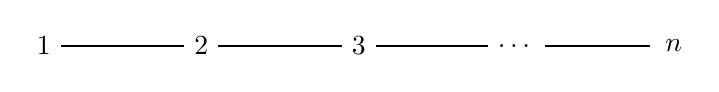
\begin{tikzpicture}[>= stealth, shorten >=2pt, line width =0.5 pt,
			node distance=2 cm]
		\node  at (0,0) (one) {$ 1 $};
		\node [right of=one] (two) {$ 2 $};
		\node [right of=two] (three) {$ 3 $};
		\node [right of=three] (dots) {$\dots$};
		\node [right of=dots] (n) {$n$};

		\draw (one) -- (two) -- (three) -- (dots) -- (n);
	\end{tikzpicture}
\end{center}

\section{April 2}
\tbf{Recall:} $(X_1, \dots, X_n)$ is a \emph{Gibbs Random Field} wrt a graph $F$ if
\[p(x_1, \dots, x_n) = \frac{1}{Z}\prod_{\text{cliques } c \sub G} \phi_c(x_c)\]
for clique functions $\phi_c$ and $Z$ a partition function, i.e. if $p(x_1, \dots, x_n)$ factors on $G$.

\tbf{Example (Hidden Markov Model):} Suppose we know our friend's behavior very well. Based on \emph{observations} (e.g. they choose to go for a walk, shop, or clean) we can guess a hidden state unknown to us (e.g. it is sunny or it is rainy).

Suppose the transition probability is given by
\[\begin{array}{cc}
		                 & \begin{array}{cc}
			                   \text{Sunny} & \text{Rainy}
		                   \end{array} \\
		\begin{array}{c}
			\text{Sunny} \\
			\text{Rainy}
		\end{array} & \left(\begin{array}{cc}
				                    0.7 & 0.3 \\
				                    0.4 & 0.6
			                    \end{array}\right)
	\end{array}\]

Then $\{(X_1, Y_1), \dots, (X_n, Y_n)\}$ is a Markov Chain with with emission probabilities

\qquad \begin{tabular}{r|ccc}
	$\P(Y_i = y_i \; | \; X_i= x_i)$ & Walk & Shop & Clean \\ \hline
	Sunny                            & 0.6  & 0.3  & 0.1   \\
	Rainy                            & 0.1  & 0.4  & 0.5
\end{tabular}

Further, $(X_1, \dots, X_n, Y_1, \dots, Y_n)$ is a GRF wrt $G$.

\begin{center}
	\begin{tikzpicture}[>= stealth, shorten >=2pt, line width =0.5 pt,
			node distance=2 cm]
		\node (x1) at (0, 0) {$X_1$};
		\node (x2) [right of=x1] {$X_2$};
		\node (x3) [right of=x2] {$X_3$};
		\node (dots) [right of=x3] {$\dots$};
		\node (xn) [right of=dots] {$X_n$};

		\node (y1) [below of=x1] {$Y_1$};
		\node (y2) [below of=x2] {$Y_2$};
		\node (y3) [below of=x3] {$Y_3$};
		\node (yn) [below of=xn] {$Y_n$};

		\draw (x1) -- (x2) -- (x3) -- (dots) -- (xn);

		\foreach \i in {1, 2, 3, n} {
				\draw (x\i) -- (y\i);
			}

		%\node [node distance=1cm, left of=x1] {Weather};
		%\node [node distance=1cm, left of=y1] {Activity};
	\end{tikzpicture}
\end{center}

If we assume $\P(X_1) = (0.2, 0.8)$,
\begin{align*}
	\P(\text{Sunny}, \text{Rainy}, \text{Walk}, \text{Shop}) & = \P(X_1 = \text{Sunny}, X_2 = \text{Rainy}, Y_1 = \text{Walk}, Y_2 = \text{Shop})                                                                                                            \\
	                                                         & = \P(X_1 = \text{Sunny}) \cdot \P(X_2 = \text{Rain} \; | \; X_1 = \text{Sunny}) \cdot \P(Y_1 = \text{Walk} \; | \; X_1 = \text{Sunny}) \cdot \P(Y_2 = \text{Shop} \; | \; X_2 = \text{Rainy}) \\
	                                                         & =0.2 \cdot 0.3 \cdot 0.6 \cdot 0.4                                                                                                                                                            \\
	                                                         & = 0.0144
\end{align*}

From which we deduce
\[p(x_1, \dots, x_n, y_1, \dots, y_n) = p(x_1) \cdot p(x_2 \; | \; x_1) \cdots p(x_{n-1} \; | \; x_n) \cdot p(y_1 \; | \; x_1) \cdots p(y_n \; | \; x_n)\]

\tbf{Example:}
Let $X_1, X_2 \iid \text{Bernoulli}(1/2)$ and $X_3 = X_1 \oplus X_2 = \begin{cases}
		0 & X_1 = X_2    \\
		1 & X_1 \neq X_2
	\end{cases}$.

Is $(X_1, X_2, X_3)$ a GRF wrt the following?

\begin{center}
	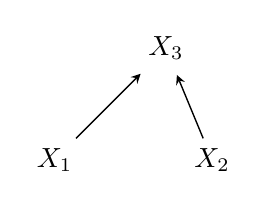
\begin{tikzpicture}[-> , >= stealth, shorten >=2pt, line width =0.5 pt,
			node distance=2 cm]
		\node (x1) at (0, 0) {$X_1$};
		\node (x2) [right of=x1] {$X_2$};
		\node (x3) [above right of=x1] {$X_3$};

		\draw (x1) -- (x3);
		\draw (x2) -- (x3);
	\end{tikzpicture}
\end{center}

We know it respects $G$ iff
\[p(x_1, x_2, x_3)  = \frac{1}{Z} f(x_1, x_3) \cdot g(x_2, x_3)\]

We can calculate:
\begin{align*}
	p(x_1, x_2, x_3) & = \P(X_1 = x_1, X_2 = x_2, X_3 = x_3)                                      \\
	                 & = \frac{1}{2} \cdot \frac{1}{2} \P(X_3 = x_3 \; | \; X_1 = x_1, X_2 = x_2) \\
	                 & = \frac{1}{4} \ind_{x_3 = x_1 \oplus x_2}
\end{align*}

Assume $\ind_{x_3 = x_1 \oplus x_2} = f(x_1, x_2) \cdot g(x_2, x_3)$.

But if $g(x_2, x_3) = 0$, then $\ind_{x_3 = x_1 \oplus x_2} = 0$ regardless of $x_1$. But by definition, for any value of $x_3 = x_1 \oplus x_2$, there exists a value of $x_1$ such that $\ind_{x_3 = x_1 \oplus x_2} = 1$. Contradiction. In particular, this means that the smallest possible graph for $(X_1, X_2, X_3)$ is the complete graph $K_3$.

\tbf{Example (Multinomial):} Roll a die 5 times giving $X_1, \dots, X_5$, the number of times we get each face. We know that $X_1 + \dots + X_6 = 5$

Which graph does this respect?
\[p(x_1, \dots, x_6) = \frac{5!}{x_1! \cdots x_6!} \cdot \frac{1}{6^5} \cdot \ind_{x_1 + \dots + x_6 = 5}\]

As before, we cannot factor this indicator, so the minimal graph is $K_6$.

\tbf{Example (Naive Bayes):} Run $d$ tests to classify $Y \in \{1, \dots, s\}$ giving data $(X_1, \dots, X_d, Y)$.


\[f(x_1, \dots, x_d, y) = p(y) p(x_1, \dots, x_d \; | \; y) \overset{NB}{=} p(y) \prod_{i=1}^d f_y(x_i) \]


\begin{exercise}
	\textbf{Exercise:} What is the minimal graph for a Naive Bayes model?

	\div

	\tbf{Solution:} By the Naive Bayes' assumption, each test is independent and only depends on the class.
	\begin{center}
		\begin{tikzpicture}[-> , >= stealth, shorten >=2pt, line width =0.5 pt,
				node distance=2 cm]
			\node (x1) at (0, 0) {$X_1$};
			\node (x2) [right of=x1] {$X_2$};
			\node (x3) [right of=x2] {$X_3$};
			\node (dots) [right of=x3] {$\dots$};
			\node (xn) [right of=dots] {$X_d$};

			\node (y) [above of=x3] {$Y$};

			\foreach \x in {1, 2, 3, n} {
					\draw (x\x) -- (y);
				}
		\end{tikzpicture}
	\end{center}


\end{exercise}

\section{April 4}
\subsection{Independence}

Suppose $(X_v)_{v \in V(G)}$ is GRF wrt $G$ where $G$ is partitioned into two disjoint sets $A$ and $B$ ($V(G) = A \cup B$) with no edges between them

\begin{center}
	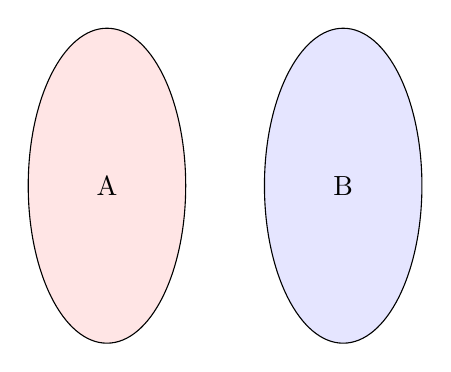
\begin{tikzpicture}
		\draw[fill=red, fill opacity=0.1] (0, 0) ellipse (1 and 2) node [black, opacity=1]{A};
		\draw[fill=blue, fill opacity=0.1] (3, 0) ellipse (1 and 2) node[black, opacity=1]{B};
	\end{tikzpicture}
\end{center}
then $(X_v)_{v \in A} \perp (X_u)_{u \in B}$ so we say $(X_v)_{v \in A}$ and $(X_u)_{u \in B}$ are \emph{independent}.

\tbf{Example:} Let $X_1, \dots, X_5$ respect

\begin{center}
	\begin{tikzpicture}[node distance=2cm]
		\node (1) at (0,0) {1};
		\node[above right of=1] (2) {2};
		\node[below right of=1] (3) {3};

		\node[right of=2] (4) {4};
		\node[below of=4] (5) {5};

		\draw (1) -- (2) -- (3) -- (1);
		\draw (4) -- (5);
	\end{tikzpicture}
\end{center}

\begin{tbox}{\textbf{Claim:} $(X_1, X_2, X_3) \perp (X_4, X_5)$}
	\emph{Proof:} $x_A \perp x_B$ iff $p(x_A, x_B) = p(x_A)p(x_B)$.

	We have
	\[p(x_A, x_B) = \frac{1}{Z} \prod_{c \text{ cliques}} f_c(x_c)\]
	by definition of GRF.

	Notice that any clique in $A$ must be entirely contained in $A$ (and similarly for $B$). Hence,
	\begin{align*}
		p(x_A, x_B) & = \frac{1}{Z} \prod_{\begin{subarray}{gather*}
				                                   c \text{ cliques}\\
				                                   c \sub A
			                                   \end{subarray}} f_c(x_c) \cdot \prod_{\begin{subarray}{gather*}
				                                                                         c \text{ cliques}\\
				                                                                         c \sub B
			                                                                         \end{subarray}} f_c(x_cz) \\
		            & = \frac{1}{Z} f_A(x_A) \cdot f_B(x_B)
	\end{align*}

	But since $Z$ is a normalization factor,
	\[Z = \sum_{x_A} \sum_{x_B} f_A(x_A) f_B(x_B) = \sum_{x_A} f_A(x_A) \left[\sum_{x_B} f_B(x_B)\right]= \left[\sum_{x_A} f_A(x_A)\right] \left[\sum_{x_B} f_B(x_B)\right] = Z_A \cdot Z_B\]

	So
	\[p(x_A, x_B) = \left[\frac{1}{Z} f_A(x_A)\right] \left[\frac{1}{Z_B} f_B(x_B)\right] = p_A(x_A) \cdot p_B(x_B)\]
	for pmfs $p_A, p_B$.

\end{tbox}

\tbf{Example:} Consider a case with three sets $A, B, D$ with no edges between $A, B$ but edges between $A, D$ and $B, D$. Now is it true that $A \perp B$?

\begin{center}
	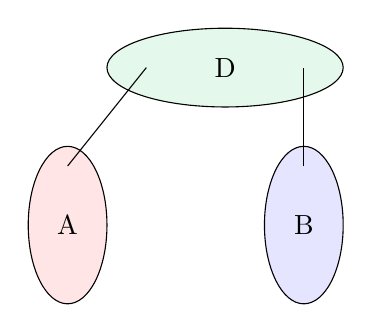
\begin{tikzpicture}
		\draw[fill=red, fill opacity=0.1] (0, 0) ellipse (0.5 and 1) node [black, opacity=1]{A};
		\draw[fill=blue, fill opacity=0.1] (3, 0) ellipse (0.5 and 1) node[black, opacity=1]{B};
		\draw[fill=mygreen, fill opacity=0.1] (2, 2) ellipse (1.5 and 0.5) node[black, opacity=1]{D};

		\draw (0, 0.75) -- (1, 2);
		\draw (3, 0.75) -- (3, 2);
	\end{tikzpicture}
\end{center}

Consider a simple case:
\begin{center}
	\begin{tikzpicture}[node distance=2cm]
		\node (1) at (0,0) {1};
		\node[right of=1] (2) {2};
		\node[right of=2] (3) {3};

		\draw (1) -- (2) -- (3);
	\end{tikzpicture}
\end{center}

If this is a Markov chain, then there are no edges between $X_1$ and $X_2$ but there is certainly still a dependence between them.

Is there a sufficient condition to conclude $A \perp B$? Clearly, we just need there to not exist a path between $A$ and $B$.

\begin{proof}
	\emph{Proof:} Suppose there is no path between $A$ and $B$.

	Let
	\begin{align*}
		\tilde A & = \{v: \exists \text{ path from } v \text{ to } A\} \\
		\tilde B & = V \setminus \tilde A
	\end{align*}

	Clearly, $\tilde A \cap \tilde B = \emptyset$ and $A \sub \tilde A$, $B \sub \tilde B$ since they share no edges.

	But $X_{\tilde A} \perp X_{\tilde B} \implies X_A \perp X_B$.
\end{proof}

To summarize:
\begin{itemize}
	\item No edges $\notimplies$ independence
	\item Independence $\notimplies$ no edges (even on a minimal graph!)
	\item No path $\implies$ independence
\end{itemize}

\subsection{Conditioning}

Suppose $(X_v)_{v \in V}$ respects $G$ conditioned on $(X_v)_{v \notin A}$.
\begin{center}
	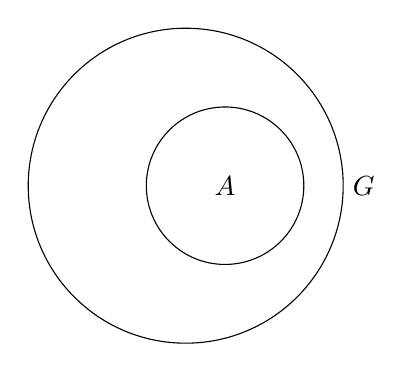
\begin{tikzpicture}
		\draw (0, 0) circle (2);
		\node[right] at (2, 0) {$G$};

		\draw (0.5, 0) circle (1) node {$A$};
	\end{tikzpicture}
\end{center}

\tbf{Conditioning:} What graph does $(X_v)$ respect?

\tbf{Marginalizing:} What graph does $(X_A)$ respect?

\tbf{Example:} Let $X \sim \text{Bernoulli}(1/2)$ and $Y = 1 - X$.
\begin{enumerate}
	\item Conditioned on $X$, what is the distribution of $Y$? Answer: fixed point, since there is no randomness
	\item What is the marginal distribution of $Y$? Answer: $\text{Bernoulli}(1/2)$
\end{enumerate}

\tbf{Example:} Let $G$ be
\begin{center}
	\begin{tikzpicture}[node distance=1cm]
		\node (1) at (0,0) {1};
		\node[above right of=1] (2) {2};
		\node[below right of=2] (3) {3};

		\draw (1) -- (2) -- (3);
	\end{tikzpicture}
	and define $A = \{1, 3\}$.

	Conditioned on $X_2$, what graph does $(X_n)$ represent? What graph respects the marginal distribution of $X_A$?

	\emph{Answer:}

	\begin{itemize}
		\item The conditioned graph is

		      \begin{center}
			      \begin{tikzpicture}
				      \node (1) at (0, 0) {$\bullet$};
				      \node (2) at (2, 0) {$\bullet$};

				      \node[below left of=1] {$1$};
				      \node[below right of=2] {$3$};

			      \end{tikzpicture}
		      \end{center}

		\item The marginal graph is
		      \begin{center}
			      \begin{tikzpicture}
				      \node (1) at (0, 0) {$\bullet$};
				      \node (2) at (2, 0) {$\bullet$};

				      \node[below left of=1] {$1$};
				      \node[below right of=2] {$3$};

				      \draw (1) -- (2);
			      \end{tikzpicture}
		      \end{center}
	\end{itemize}
\end{center}

\tbf{Remark:} While this marginal graph works, it is the worst case graph. i.e., in most cases there is a smaller graph possible.

\begin{proposition}
	\textbf{Theorem:}
	\begin{itemize}
		\item Conditioning: $G_1$ is the reduced subgraph of $G$ on $A$:
		      $G_1 = (A, E_A)$ where $E_A = E(G) \cap (A \times A)$. (That is, edges in $G_1$ are simply edges in $G$ restricting on $A$.
		\item Marginalizing: $G_2 = (A, E_2(A))$ defined by $(u, v) \in E_2(A)$ if $u \sim v$ or $u, v$ connected by a path outside $A$.
	\end{itemize})
\end{proposition}

\tbf{Example:} Let $G$ be
\begin{center}
	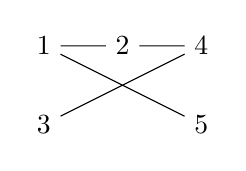
\begin{tikzpicture}[node distance=1cm]
		\node (1) at (0, 0) {1};
		\node[right of=1] (2) {2};
		\node[below of=1] (3) {3};
		\node[right of=2] (4) {4};
		\node[below of=4] (5) {5};

		\draw (5) -- (1) -- (2) -- (4) -- (3);
	\end{tikzpicture}
\end{center}

Then for $A = \{1, 2, 3\}$,

\begin{center}
	\begin{tabular}{c|c}
		$G_1$                                  & $G_2$            \\ \hline
		\begin{tikzpicture}[node distance=1cm]
			\node (1) at (0, 0) {1};
			\node[right of=1] (2) {2};
			\node[below right of=1] (3) {3};

			\draw (1) -- (2);
		\end{tikzpicture} & \begin{tikzpicture}[node distance=1cm]
			                    \node (1) at (0, 0) {1};
			                    \node[right of=1] (2) {2};
			                    \node[below right of=1] (3) {3};

			                    \draw (1) -- (2) -- (3);
		                    \end{tikzpicture}
	\end{tabular}
\end{center}

\section{April 7}

\begin{tbox}{\textbf{Theorem:} Let  $(X_v)_{v \in G}$ be aGRF wrt a graph $G$ if $A \sub V(G)$. Conditioned on $X_{A^c}$, the rv $X_A$ is a GRF wrt the induced graph on $A$, i.e. $v \overset{G'}{\sim} u$ in this graph iff $v, u \in A$ and $v\overset{G}{\sim} u$. }
	\emph{Example:} Let $G$ be
	\begin{center}
		\begin{tikzpicture}[node distance=1cm]
			\node (1) at (0, 0) {1};
			\node[above right of=1] (3) {3};
			\node[below right of=1] (2) {2};
		\end{tikzpicture}
	\end{center}
	and $A = \{1, 2\}$ so $G = (\{1, 2\}, \emptyset)$.

	\emph{Proof for the example:} Take $X_1, X_2, X_3$ from the joint distribution. Then
	\begin{align*}
		p(x_1, x_2, x_3) & = \frac{1}{Z}\phi_1(x_1) \phi_2(x_2) \phi_{12}(x_1, x_2) \phi_{13}(x_1, x_3) \phi_{23}(x_2, x_3) \\
		                 & = \frac{1}{Z} f_{13}(x_1, x_3) \cdot f_{23}(x_2, x_3)
	\end{align*}

	\div

	\emph{Proof for the General Case:} Suppose $(X_v)$ is a GRF wrt $G$ so
	\[p(x_1, \dots, x_n) = \frac{1}{Z} \prod_{c\text{ cliques}} \phi_c(x_c) = \frac{1}{Z} \prod_{c \text{ cliques}} \phi_c(x_{A \cap C, x_{A^c \cap C}})\]
	for any $C$ satisfying $C = (A \cap C) \cup (A^c \cap C)$ (i.e. the measurable sets $C$)

	Fix $x_{A^c}$ so
	\[\P_{x_A \; | \; X_{A^c = x_{A^c}}}(x_A) = \frac{\P(X_A = x_A, X_{A^c} = x_{A^c})}{\P(X_{A^c} = x_{A^c})}\]
	but notice the denominator does not depend on $x_A$ so we can call it a constant $Z'$.

	Then,
	\begin{align*}
		\frac{\P(X_A = x_A, X_{A^c} = x_{A^c})}{Z'} & = \frac{\frac{1}{Z} \prod_{c \text{ cliques}} \phi_c(x_{A \cap C}, x_{A^c \cap C})}{Z'}                                                                                                                 \\
		                                            & = \frac{1}{Z \cdot Z'} \overbrace{\left[\prod_{\text{cliques } C \sub A^c} \phi_c(c_{A^c \cap C})\right]}^{Z''}\left[\prod_{\text{cliques } C \not\sub A^c} \phi_c(x_{A \cap C}, x_{A^c \cap C})\right] \\
		                                            & = \frac{Z''}{ZZ'} \prod_{\text{cliques } C \cap A \neq \emptyset} \phi_c(x_{A \cap C}, x_{A^c \cap C})
	\end{align*}

	\begin{center}
		\begin{tikzpicture}[node distance=1cm]
			\draw (0, 0) circle (2);
			\draw (0, -2) -- (0, 2);

			\draw (-0.5, -0.5) rectangle (0.5, 0.5);
			\draw (-0.5, -0.5) -- (0.5, 0.5);
			\draw (0.5, -0.5) -- (-0.5, 0.5);

			\node at (-1, 0) {$A$};
			\node at (1, 0) {$A^c$};
		\end{tikzpicture}
	\end{center}

	Since $\phi_c(x_{A\cap C}, x_{A^c \cap C})$ is a function on the clique $C \cap A$, $p(x_A)$ can be factored into cliques.

\end{tbox}

\tbf{Definition 1:} $(X_v)$ is a GRF wrt $G$ if
\[p(x_v) = \frac{1}{Z} \prod_{c \text{ cliques}} \phi_c(x_c)\]

\tbf{Definition 2:} $(X_v)$ is a GRF wrt $G$ if
\[p(x_v) = \frac{1}{Z} \prod_{c \text{ maximum cliques}} \phi_c(x_c)\]

Hence,
\begin{align*}
	p(x_1, x_2 \; | \; x_3) & = \frac{1}{Z'_{x_3}} f_{13, x_3}(x_1) \cdot f_{23, x_3}(x_2) \\
	                        & = \frac{\P(X_1= x_1, X_2= x_2, X_3 = x_3)}{\P(X_3 = x_3)}
\end{align*}

\emph{Example:}
\begin{align*}
	X_1 & \sim \text{Bernoulli}(1/2)     \\
	X_3 & = X_1 + \text{Bernoulli}(0.01) \\
	X_2 & = X_3 + \text{Bernoulli}(0.9)  \\
\end{align*}
gives
\begin{align*}
	X_1 & \sim \begin{cases}
		           0 & \text{with prob } 0.5 \\
		           1 & \text{with prob } 0.5
	           \end{cases}         \\
	X_3 & = \begin{cases}
		        0 & \frac{1}{2} \cdot \frac{99}{100} \\
		        1 & \frac{1}{2}                      \\
		        2 & \frac{1}{2} \cdot \frac{1}{100}
	        \end{cases} \\
	X_2 & = \begin{cases}
		        0 \\
		        1 \\
		        2 \\
		        3
	        \end{cases}
\end{align*}

\[p(x_1, x_2, x_3) = \frac{1}{Z} f_{13}(x_3, x_1) \cdot f_{23}(x_2, x_3)\]

Conditioned on $X_3 = 0$,
\[p(x_1, x_2) = p_{x_3=0}(0, 1) = \frac{\P(X_1 =0, X_2 = 1, X_3 = 0)}{\P(X_3 = 0)} = \frac{\P(0, 1, 0)}{\sum_{x, y} \P(x, y, 0)} = \frac{1}{Z}f_{13}(0, 0) = \frac{f_{23}(1, 0)}{Z'}\]

\tbf{Example (Naive Bayes):}

\begin{center}
	\begin{tikzpicture}[node distance=2cm]
		\node (y) at (0, 0) {$y$};
		\node[above right of=y] (1) {$X_1$};
		\node[right of=y, node distance=1.5cm] (2) {$\vdots$};
		\node[below right of=y] (d) {$X_d$};

		\foreach \i in {1, 2, d} {
				\draw (y) -- (\i);
			}
	\end{tikzpicture}
\end{center}

Conditioned on $Y$, the distribution of $X_1, \dots, X_d$ is $(X_1, \dots, X_d) \sim \text{Multinomial}(p_1, \dots, p_d)$.

\tbf{Example (Hidden Markov Model):}

\begin{center}
	\begin{tikzpicture}[node distance=2cm]
		\node (x1) at (0, 0) {$X_1$};
		\node[right of=x1] (x2) {$X_2$};
		\node[right of=x2] (x3) {$X_3$};
		\node[right of=x3] (dots) {$\dots$};
		\node[right of=dots] (xd) {$X_d$};

		\node[below of=x1] (y1) {$Y_1$};
		\node[below of=x2] (y2) {$Y_2$};
		\node[below of=x3] (y3) {$Y_3$};
		\node[below of=xd] (yd) {$Y_d$};

		\draw (x1) -- (x2) -- (x3) -- (dots) -- (xd);
		\foreach \i in {1, 2, 3, d} {
				\draw (x\i) -- (y\i);
			}
	\end{tikzpicture}
\end{center}

Conditioned on $Y_1, \dots, Y_d$, the distribution of $X_1, \dots, X_d$ is

\begin{center}
	\begin{tikzpicture}[node distance=2cm]
		\node (x1) at (0, 0) {$X_1$};
		\node[right of=x1] (x2) {$X_2$};
		\node[right of=x2] (x3) {$X_3$};
		\node[right of=x3] (dots) {$\dots$};
		\node[right of=dots] (xd) {$X_d$};

		\draw (x1) -- (x2) -- (x3) -- (dots) -- (xd);
	\end{tikzpicture}
\end{center}

Conditioned on $X_1, \dots, X_d$ the distribution of $Y_1, \dots, Y_d$ is

\begin{center}
	\begin{tikzpicture}[node distance=2cm]
		\node (y1) at (0, 0) {$Y_1$};
		\node[right of=y1] (y2) {$Y_2$};
		\node[right of=y2] (y3) {$Y_3$};
		\node[right of=y3] (dots) {$\dots$};
		\node[right of=dots] (yd) {$Y_d$};
	\end{tikzpicture}
\end{center}
that is, they are independent.

\begin{tbox}{\textbf{Theorem (Marginalizing):} Let the marginal distribution of $(X_A)$ be a GRF wrt $G''=(A, E'')$. Then for $u, v \in A$,
		\[u \overset{E''}{\sim} v \impliedby \begin{cases}
				u \overset{G}{\sim} v \\
				\text{there exists a path between } u \text{ and } v \text{ entirely in } A^c
			\end{cases}\]  }
	\emph{Example:}

	\begin{center}
		\begin{tikzpicture}[node distance=2cm]
			\node (1) at (0, 0) {1};
			\node[above right of=1] (2) {2};
			\node[below right of=2] (3) {3};
			\node[above right of=3] (5) {5};
			\node[above of=2] (4) {4};

			\draw (1) -- (2) -- (3) -- (5) -- (4) -- (1);
		\end{tikzpicture}
	\end{center}
	with $A = \{1, 2, 3, 5\}$ we have the subgraph

	\begin{center}
		\begin{tikzpicture}[node distance=2cm]
			\node (1) at (0, 0) {1};
			\node[above right of=1] (2) {2};
			\node[below right of=2] (3) {3};
			\node[above right of=3] (5) {5};

			\draw (1) -- (2) -- (3) -- (5) to[bend left, out=90, in=90] (1);
		\end{tikzpicture}
	\end{center}

	\emph{Proof of theorem for the example:}
	\begin{align*}
		p(x_1, x_2, x_3, x_5)   & = \sum_{x_4} p(x_1, x_2, x_3, x_4, x_5)                                                                                   \\
		                        & = \sum_{x_4} \frac{1}{Z} \phi_{12}(x_1, x_2) \phi_{23}(x_2, x_3) \phi_{35}(x_3, x_5) p_{14}(x_1, x_4) \phi_{45}(x_4, x_5) \\
		\sum_{x_4} p_{14}p_{45} & = f(x_1, x_5)
	\end{align*}

	\div

	\emph{Proof Sketch:}
	\[p_{X_A}(x_A) = \P(X_A = x_A) = \sum_{x_{A^c}} \P(x_A, x_{A^c})\]
	but we know
	\begin{align*}
		p(x_1, \dots, x_n) & = \frac{1}{Z} \prod_{\text{cliques } c \sub G} \phi_c(x_c)                                         \\
		                   & = \frac{1}{Z} \sum_{x_{A^c}} \prod_{\text{cliques } c \sub G} \phi_c(x_{c \cap A}, x_{C \cap A^c}) \\
		                   & \overset{?}{=} \frac{1}{Z'} \prod_{\text{cliques } c \sub G''} \phi_c(x_{C \cap A})
	\end{align*}

	\begin{exercise}
		\textbf{Exercise:} Prove the theorem for the general case.
	\end{exercise}
\end{tbox}

\tbf{Example:} For

\begin{center}
	\begin{tikzpicture}[node distance=1cm]
		\draw (0, -1) circle (2);

		\draw (-0.5, -0.5) rectangle (0.5, 0.5);
		\draw (-0.5, -0.5) -- (0.5, 0.5);
		\draw (0.5, -0.5) -- (-0.5, 0.5);

		\node[below left] at (-0.5, -0.5) {1};
		\node[above left] at (-0.5, 0.5) {1};
		\node[below right] at (0.5, -0.5) {1};
		\node[above right] at (0.5, 0.5) {1};
	\end{tikzpicture}
\end{center}
and fixed $c$,
\[\sum_{x_{34}} \phi_c(x_{12}, x_{34}) = \phi_{12}(x_{12})\]

\tbf{Example (Naive Bayes):} The marginal distribution of $(X_i)$ is the complete graph

\begin{center}
	\begin{tikzpicture}[node distance=2cm]
		\node (y) at (0, 0) {$y$};
		\node[above right of=y] (1) {$X_1$};
		\node[right of=y, node distance=1.5cm] (2) {$\vdots$};
		\node[below right of=y] (d) {$X_d$};

		\foreach \i in {1, 2, d} {
				\draw (y) -- (\i);
			}
	\end{tikzpicture}
\end{center}

\tbf{Example (Hidden Markov Model):} If we were to condition on the observations $(Y_i)$, then we would have a Markov chain. However, the marginal distribution on $Y_1, \dots, Y_d$ is the complete graph

\subsection{Markov Random Fields}
\tbf{Markov Random Field:} $(X_v)_{v \in G}$ is a \emph{Markov Random Field} (MRF) if
\[\P(X_i = x_i \; | \; X_{i^c} = x_{i^c}) = \P(X_i = x_i \; | \; x_{N_i} = x_{N_i})\]
where $N(i) = \{j: (j, i) \in E\}$ is the neighborhood of $i$.

\tbf{Example:}

\begin{center}
	\begin{tikzpicture}[node distance=2cm]
		\node (1) at (0, 0) {1};
		\node[above right of=1] (2) {2};
		\node[below right of=1] (3) {3};
		\node[above right of=3] (4) {4};

		\draw (1) -- (2) -- (3) -- (1);
		\draw (3) -- (4);
	\end{tikzpicture}
\end{center}

\[\P(X_1 = x_1 \; | \; X_2 = x_2, X_3 = x_3, X_4 = x_4) = \P(X_1 = x_1 \; | \; X_2= x_2, X_3 = x_3)\]

\begin{tbox}{\textbf{Theorem (Hammersley-Clifford):} Assume $(X_v)$ is positive (i.e. $p(x_1, \dots, x_n) > 0$ for all $x_1, \dots, x_n \in \Omega_1 \times \dots \times \Omega_n$). Then $X$ is a Gibbs Random Field iff it is a Markov Random Field. }
	\emph{Proof:} (GRF $\implies$ MRF) Conditioned on $X_{N(i)}$, the distribution of is $A = \{i\} \cup \{j: j \notin N(i)\}$ from which it immediately follows that $i \perp \{j: j \notin N(i)\}$ hence
	\[\P(X_i = x_i \; | \; X_{N_i}, \dots) =\P(X_i = x_i \; | \; X_{N_i})\]

	\div

	The other direction is highly non-trivial.
\end{tbox}

\subsection{Computing Grpahical Models}
To use any graphical model
\[p(x_1, \dots, x_n) = \frac{1}{Z} \prod_c \phi_c(x_c)\]
we need to know
\[Z = \sum_{x_1, \dots, x_n} \prod_c \phi_c(x_c)\]
which is very difficult in practice.

\tbf{Example:}

\begin{center}
	\begin{tikzpicture}[node distance=2 cm]
		\node (1) at (0, 0) {1};
		\node[right of=1] (2) {2};
		\node[right of=2] (3) {3};
		\node[below of=$2!0.5!3$] (4) {4};
		\node[right of=3] (5) {5};
		\node[right of=5] (6) {6};

		\draw (1) -- (2) -- (3) -- (5) -- (6);
		\draw (2) -- (4) -- (3);
	\end{tikzpicture}
\end{center}

Recall that we can specify $p$ by the product of all the cliques or just the maximum cliques:
\[p(x_1, \dots, x_6) = \frac{1}{Z} \phi_{12}(x_{12}) \phi_{234}(x_{234}) \phi_{25}(x_{35}) \phi_{56}(x_{56})\]

Since $\sum_{x_1, \dots, x_6} p = 1$,
\begin{align*}
	Z & = \sum_{x_1, \dots, x_6} \phi_{12}(x_{12}) \phi_{234}(x_{234}) \phi_{25}(x_{35}) \phi_{56}(x_{56})                                                                                             \\
	  & = \sum_{x_6} \sum_{x_5} \sum_{x_4} \sum_{x_3} \sum_{x_2} \sum_{x_1} \phi_{12}(x_{12}) \phi_{234}(x_{234}) \phi_{25}(x_{35}) \phi_{56}(x_{56})                                                  \\
	  & = \sum_{x_6} \left(\sum_{x_5} \phi_{56}(x_{56}) \left(\sum_{x_3} \phi_{35}(x_{35}) \left(\sum_{x_4, x_2} \phi_{234}(x_{234}) \left(\sum_{x_1} \phi_{12}(x_{12})\right) \right) \right) \right) \\
	  & = \sum_{x_6} \left(\sum_{x_5} \phi_{56}(x_{56}) \left(\sum_{x_3} \phi_{35}(x_{35}) \left(\sum_{x_4, x_2} \phi_{234}(x_{234}) T_1(x_2)\right) \right) \right)                                   \\
	  & = \sum_{x_6} \left(\sum_{x_5} \phi_{56}(x_{56}) \left(\sum_{x_3} \phi_{35}(x_{35}) T_2(x_3) \right)\right)                                                                                     \\
	  & = \sum_{x_6} \left(\sum_{x_5} \phi_{56}(x_{56}) T_3(x_5)\right)                                                                                                                                \\
	  & = \sum_{x_6} T_5(x_6)                                                                                                                                                                          \\
	  & = T_6
\end{align*}

We can calculate
\qquad \begin{tabular}{r|c}
	           & cost             \\\hline
	$T_1(x_2)$ & $\abs{\Omega}^2$ \\
	$T_2(x_3)$ & $\abs{\Omega}^3$ \\
	$T_3(x_5)$ & $\abs{\Omega}^2$ \\
	$T_4(x_5)$ & $\abs{\Omega}^2$ \\
	$T_5(x_6)$ & $\abs{\Omega}^2$ \\
	$T_6$      & $\abs{\Omega}^1$ \\
\end{tabular}

giving total cost $\abs{\Omega} + 4\abs{\Omega}^2 + \abs{\Omega}^3$ where the cost is calculated by $\abs{\Omega}^{\# \text{new neighbors} +  1}$ in the graph.

\section{April 11}
Let
\[p(x) = \frac{1}{Z} \phi_1(x_1)\phi_{12}(x_{12})\phi_{23}(x_{23})\phi_5(x_5) \phi_{56}(x_{56})\]
on
\begin{center}
	\begin{tikzpicture}[node distance=2 cm]
		\node (1) at (0, 0) {1};
		\node[right of=1] (2) {2};
		\node[right of=2] (3) {3};
		\node[below right of=2] (4) {4};
		\node[right of=3] (5) {5};
		\node[right of=5] (6) {6};

		\draw (1) -- (2) -- (3) -- (5) -- (6);
		\draw (2) -- (4) -- (3);
	\end{tikzpicture}
\end{center}

If we visit the vertices in the order $1, 2, 3, 4, 5, 6$, we can calculate costs
\begin{center}
	\begin{tikzpicture}[node distance=2 cm]
		\node (1) at (0, 0) {$\abs{\Omega}^2$};
		\node[right of=1] (2) {$\abs{\Omega}^3$};
		\node[right of=2] (3) {$\abs \Omega^3$};
		\node[below right of=2] (4) {$\abs{\Omega}^2$};
		\node[right of=3] (5) {$\abs \Omega^2$};
		\node[right of=5] (6) {$\abs \Omega^1$};

		\draw (1) -- (2) -- (3) -- (5) -- (6);
		\draw (2) -- (4) -- (3);
	\end{tikzpicture}
\end{center}
giving total $\abs{\Omega} + 3\abs \Omega^2 + 2\abs \Omega^3$

by letting the currectly visited vertex $v_k$ having visited $v_1, \dots, v_{k-1}$ with cost $\abs{\Omega}^{D_A + 1}$ where
\begin{align*}
	A   & = [n] \setminus \{v_1, \dots, v_k\}                        \\
	D_A & = \partial A =\{u \in A: \exists v \notin A, \; u \sim v\}
\end{align*}

Notice, though, that if we visit the vertices instead in the order 1, 2, 4, 3, 5, 6, we have cost
\[\abs{\Omega}^2 + \abs{\Omega}^3 + \abs \Omega^2 + \abs \Omega^2 + \abs \Omega^1= \abs \Omega + 4\abs \Omega^2 + \abs \Omega^3 \]
which is much better. We call this the \tbf{boundary trick}.

\begin{tbox}{\textbf{Marginalization Theorem:} Let the marginal distribution of $(X_A)$ be a GRF wrt $G''=(A, E'')$. Then for $u, v \in A$,
		\[u \overset{E''}{\sim} v \impliedby \begin{cases}
				u \overset{G}{\sim} v \\
				\text{there exists a path between } u \text{ and } v \text{ entirely in } A^c
			\end{cases}\]
	}
	\emph{Proof:} Suppose $A^c$ has connected components $D_1, \dots, D_k$. Denote $M_1 = D_1 \cup \underbrace{N(D_1)}_{\sub A}$.

	What can we say about $N(D_1)$? Since $D_1$ is connected, we know that there must be a path between points $u, v$ in $D_1$. By definition, $u \overset{N(D_1)}{\sim} v$ so $N(D_1)$ must be a complete graph.

	\tbf{Observation 1:} $\forall i$, $N(D_i)$ is complete in $G''$

	\tbf{Observation 2:} Every clique $C$ in $G$ must either be in the induced graph $A$ or $M_i$ for some $i$.

	For $X_v$ a GRF,
	\begin{align*}
		p(x_V) & = \frac{1}{Z} \prod_{c \sub G} \phi_c(x_c)                                                                                                                \\
		p(x_A) & = \sum_{x_{A^c}} p(x_A, x_{A^c})                                                                                                                          \\
		       & = \frac{1}{Z} \sum_{x_{A^c}} \prod_{c \sub G} \phi_c(x_{A\cap C}, c_{A^c \cap C})                                                                         \\
		       & = \frac{1}{Z} \sum_{x \in D_1} \sum_{x \in D_2}\dots \sum_{x \in D_k} \prod_{c \sub G} \phi_c(x_{A\cap C}, x_{A^c \cap C})                                \\
		       & = \frac{1}{Z}\prod_{i=1}^k\left[\sum_{x \in D_i} \prod_{\begin{subarray}{c}
					                                                                 c \sub G \\
					                                                                 c \cap D_i \neq \emptyset
				                                                                 \end{subarray}} \phi_c(x_{A \cap C}, x_{A^c \cap C})\right] \prod_{c \sub A} \phi_c(x_{c \cap A})
	\end{align*}

	For each $i = 1: k$,
	\[\sum_{x \in D_i} \prod_{\begin{subarray}{c}
				c\in G\\
				c \cap D_i \neq \emptyset
			\end{subarray}} \phi_c(x_{A\cap C}, x_{A^c \cap c}) = \phi_{N(D_i)}(x_{N(D_i)})\]
	where $N(D_u)$ is a clique in $G'$
\end{tbox}

\tbf{Example:}

\begin{center}
	\begin{tikzpicture}
		\node (1) at (0, 0) {1};
		\node[right of=1] (2) {2};
		\node[right of=2] (3) {3};
		\node[below right of=3] (4) {4};
		\node[below of=2] (5) {5};
		\node[below left of=1] (6) {6};

		\draw (6) -- (2) -- (5) -- (4) -- (3) -- (2);
	\end{tikzpicture}
\end{center}

With $A = \{1 2, 3, 5\}$, $D_1 =\{4\}$ and $D_2=  \{6\}$ so
\begin{align*}
	\frac{1}{Z} \sum_{x_4} \sum_{x_6} \prod_c \phi(x_{A \cap c}, x_{A^c \cap c}) & = \frac{1}{Z} \sum_{x_4} \sum_{x_6} \left(\prod_{c \in \{12, 23, 25\}}
	\phi(x_{1235})\right) \left(\prod_{c \in \{34, 54\}} \phi(x_{12356})\right)
\end{align*}
and
\[\sum_{x_4} \prod_{c \in \{34, 45\}} \phi_c(x_{A \cap c}, x_{A^c\cap c}) = \phi_{35}\]

\section{April 14}
Suppose we know
\[p(x_1, \dots, x_n) = \frac{1}{Z} \prod_c \phi_c(x_c)\]
where we know $\phi_c$ but do not know $Z$. How do we sample from $p$?

\subsection{Dynamic Programming}
One method is \tbf{Dynamic Programming}:
\[Z = \sum_{x_v} \prod_c \phi_c(x_c)\]
This is advantangeous because it allows exact calculation of $Z$ but is very slow in practice. (Recall that on the graphs last week this method had $O(\abs{\Omega}^3)$ time. )

Consider if we were on an $n \times n$ lattice

\begin{center}
	\begin{tikzpicture}[node distance=1cm]
		\foreach \i in {0, 1, 2} {
				\foreach \j in {0, 1, 2} {
						\node (\i\j) at (\i, -\j) {$\bullet$};
					}
			}

		\draw (00) -- (01) -- (02);
		\draw (10) -- (11) -- (12);
		\draw (20) -- (21) -- (22);
		\draw (00) -- (10) -- (20);
		\draw (01) -- (11) -- (21);
		\draw (02) -- (12) -- (22);

		\node[right of=21] {$\dots$};
		\node[below of=12] {$\vdots$};
	\end{tikzpicture}
\end{center}

Letting $G = (V, E)$ and $V = \{(i, j): 1 \leq i, j \leq n\}$ we have $n^2$ vertices and $2n^2$ edges.

In this case, calculating $Z$ directly on only $\Omega = \{\pm 1\}$ would require a sum over $2^{n^2}$ distributions and exponential time.

In any case, how do we use dynamic programming to sample from $p$? One easy way is to
\begin{enumerate}
	\item Sample $X_1$
	\item Sample $X_2 \; | \; X_1$
	\item Sample $X_n \; | \; X_1, \dots, X_{n-1}$.
\end{enumerate}

Using this method, we only need to use the arrays $T_i$ that we got from calculating $Z$.

\tbf{Example:} With graph
\begin{center}
	\begin{tikzpicture}[node distance=2 cm]
		\node (1) at (0, 0) {1};
		\node[right of=1] (2) {2};
		\node[right of=2] (3) {3};
		\node[below right of=2] (4) {4};
		\node[right of=3] (5) {5};
		\node[right of=5] (6) {6};

		\draw (1) -- (2) -- (3) -- (5) -- (6);
		\draw (2) -- (4) -- (3);
	\end{tikzpicture}
\end{center}
and GRF
\[p(x_1, \dots, x_6) = \frac{1}{Z} \phi_{12} \phi_{234} \phi_{35} \phi_{56}\]
we have
\begin{align*}
	Z & = \sum_{x_6} \sum_{x_5} \sum_{x_3} \sum_{x_4} \sum_{x_2} \sum_{x_1} \phi_{12} \phi_{234} \phi_{35} \phi_{56}                                                                                                                                                 \\
	  & = \underbrace{\sum_{x_6} \underbrace{\sum_{x_5} \phi_{56} \underbrace{\sum_{x_3} \phi_{35} \underbrace{\sum_{x_4} \underbrace{\sum_{x_2} \phi_{234} \underbrace{\sum_{x_1} \phi_{12}}_{T_1(x_2)}}_{T_2(x_{34})}}_{T_3(x_{3})}}_{T_4(x_5)}}_{T_5(x_6)}}_{T_6} \\
\end{align*}

Before writing down the conditional distribution, let's write down the joint distribution
\begin{align*}
	p(x_1, \dots, x_6)             & = \frac{1}{Z} \phi_{12} \phi_{234} \phi_{35} \phi_{56} \\
	p(x_2, \dots, x_6)             & = \sum_{x_1} p(x_1, \dots, x_6)                        \\
	                               & = \frac{1}{Z} \phi_{234} \phi_{35} \phi_{56} T_1(x_2)  \\
	p(x_1 \; | \; x_2, \dots, x_6) & = \frac{p(x_1, \dots, x_6)}{p(x_2, \dots, x_6)}        \\
	                               & = \frac{\phi_{12}}{T_1(x_2)}
\end{align*}

Similarly over the other vertices,
\begin{align*}
	p(x_3, \dots, x_6)             & = \sum_{x_2} p(x_2, \dots, x_6)               \\
	                               & = \frac{1}{Z} \phi_{35} \phi_{56} T_2(x_{34}) \\
	p(x_2 \; | \; x_3, \dots, x_6) & = \frac{\phi_{234} T_1(x_2)}{T_2(x_{34})}     \\
	p(x_4 \; | \; x_3, \dots, x_6) & = \frac{T_2(x_{34})}{T_3(x_3)}                \\
	p(x_3 \; | \; x_5, x_6)        & = \frac{\phi_{35} T_3(x_3)}{T_4(x_5)}         \\
	p(x_5\; | \; x_6)              & = \frac{T_4(x_5)}{T_5(x_6)}                   \\
	p(x_6)                         & = \frac{\phi_{56} T_5(x_6)}{Z}
\end{align*}

\subsection{Gibbs Samplers}
Gibbs Sampling provides a cost effective alternative to dynamic program at the cost of asymptotic (rather than exact) convergence.

\tbf{Example:} Let $G$ be

\begin{center}
	\begin{tikzpicture}
		\node (1) at (0, 0) {1};
		\node[right of=1] (2) {2};
		\draw (1) -- (2);
	\end{tikzpicture}
\end{center}
so the joint distribution is
\[p(x_1, x_2) = p(X_1 = x_1, X_2 = x_2)\]

Using the\emph{ Gibbs Sampler}, let $\pi$ be any distribution on $V(G)$.
\begin{enumerate}
	\item Initialize $X_1^{(0)}, \dots, X_n^{(0)}$ to any values.
	\item Sample a vertex $i$ from $\pi$
	\item Sample $X_i \; | \; X_{i^c} \sim p(x_i \; | \; x_{i^c})$
	\item Iterate
\end{enumerate}

Now we have RVs $(X_i^{(t)})_{i \in V, t = 0, 1, 2, \dots}$. As we will see, $\text{dist}(X_1^{(t)}, \dots, X_n^{(t)}) \overset{t \to \infty}{\longrightarrow} p$.

\section{April 16}
\tbf{Markov Chain Monte Carlo:} Let $X = (X_1, \dots, X_d) \sim p$ with $p$ unknown. MCMC is an approach to sample asymptotically from $p$.

Broadly, we construct a MC $(X^{(j)})_{j = 1:T}$ according to some rule with the goal that the distribution of $x^T \to p$ as $t \to \infty$.

There are three primary methods:
\begin{enumerate}
	\item Gibbs Sampling
	\item Metropolis-Hastings
	\item Hamiltonian Monte Carlo
\end{enumerate}

\subsection{Gibbs Sampling}
Recall that we have $X = (X_1, \dots, X_d) \sim p$ and choose a distribution $\pi$ on $\{1, \dots, d\}$. We can then successively sample $X_i^T \sim p(X_i\; | \; X_j = X_j^{T-1}, \quad \forall j \neq i)$.

\tbf{Example (Ising Model):} Let $X = (X_1, \dots, X_d)$ be a sample on the $n\times n$ lattice wuth $x \in (\pm 1)^d$ and
\[p(x) = \frac{1}{Z} e^{\beta \sum_{i \sim j} x_i x_j}\]
representing the fact that $x_i x_j = 1$ if $i$ and $j$ are the same and $x_i x_j = -1$ if they are different.

Physically, this system corresponds to the interaction of spins in a metal which can aquire magnetic properties. $\beta \propto \frac{1}{\text{temp}}$ and influences the development of magnetic characteristics according to regions where spins are aligned with high probability.

We want
\begin{align*}
	p(X_i^T = 1)  & = \P(X_i = 1 \; | \; X_j = x_j \quad \forall j \neq i)                                 \\
	              & = \frac{\P(X_i = 1, X_j = x_j\; \forall j \neq i)}{\P(X_j = x_j,\; \forall j \neq i )} \\
	              & = \frac{a_1}{a_{-1}}                                                                   \\
	p(X_i^T = -1) & = \P(X_i =-1 \; | \; X_j = x_j \quad \forall j \neq i)                                 \\
\end{align*}

We can calculate
\begin{align*}
	a_1    & = \frac{1}{Z} e^{\beta \sum_{k \sim l} x_k x_l}                                                            \\
	       & = \frac{1}{Z} \exp\left(\beta \sum_{k \sim l \land k, l \neq i} x_k x_l + \beta \sum_{k \sim i} x_k\right) \\
	       & = \frac{1}{Z} e^{A + \beta H}                                                                              \\
	a_{-1} & = \frac{1}{Z} e^{A - \beta H}
\end{align*}

We want
\[\frac{a_1}{a_1 + a_{-1}} = \frac{e^A e^{\beta H}}{e^A e^{\beta H} + e^A e^{-\beta H}} = \frac{1}{1 + e^{-2\beta H}}\]

So we conluce
\begin{align*}
	\P(X^T_i = 1)  & = \frac{1}{1 + e^{-2\beta H}}     \\
	\P(X^T_i = -1) & = 1 - \frac{1}{1 + e^{-2\beta H}} \\
\end{align*}
where $H = \sum_{k \sim i} x_k$ is the sum of the neighbors of $i$.

\tbf{Remark:} Notice that this is incredibly easy to calculate and does not even require $Z$! This is the power of the Gibbs Sampler.

\begin{tbox}{\textbf{Claim:} Let $X^0, X^1, \dots$ be a Gibbs Sampler. Let $q_t$ be the distribution of $X^t$. Then $D(q_t \parallel p) \leq D(q_{t-1} \parallel p)$ for all $t$.}
	\emph{Proof:} (Assume $d= 2$).

	Let $X = (X_1, X_2)$ so $\pi$ is a distribution on $\{1, 2\}$, say $\pi = (0.3, 0.7)$.

	\begin{enumerate}
		\item Choose a vertex $v \sim \pi$
		\item Update
		      \begin{align*}
			      X_u^t = X_u^{t-1} \qquad \forall u \neq v \\
			      X_v^t \sim p(X_v \; | \; X_u = X_u^{t-1} \; \forall u \neq v)
		      \end{align*}
	\end{enumerate}

	Let $q^t$ be the distribution of $X^t$ so $q_1^t$ is the distribution of $X_1^t$. What is $q_1^t$?
	\begin{align*}
		q_1^t(x_1) & = \P(X_1^t = x_1)                                                          \\
		           & = \pi_1 \P(X_1^t = x_1\; | \; i = 1) + \pi_2 \P(X_1^t = x_1 \; | \; i = 2) \\
		           & = \pi_1 p(x_1 \; | \; x_2) + \pi_2 \P(X_1^{t-1} = x_1 \; | \; i =2)        \\
		           & = \pi_1 p(x_1 \; | \; x_2) + \pi_2 q_{t-1}(x_1)
	\end{align*}

	Hence,
	\[q_{t+1}(x_1, x_2) = \pi_1 p(x_1 \; | \; x_2) q_{t-1}(x_2) + \pi_2 p(x_2 \; | \; x_1) q_{t-1}(x_1)\]
	where
	\begin{itemize}
		\item $q_t(x_1, x_2) = \P(X_1^t = x_1, X_2^t = x_2)$
		\item $q_{t-1}(x_2) = \P(X_2^{t-1} = x_2)$
		\item $p(x_1 \; | \; x_2) = \P(X_1 = x_1 \; | \; X_2 = x_2)$
		\item $p(x_2 \; | \; x_1) = \P(X_2 = x_2 \; | \; X_1 = x_1)$
	\end{itemize}

	Let
	\begin{align*}
		r_1(x_1, x_2) & = p(x_1 \; | \; x_2) q_{t-1}(x_2) \\
		r_2(x_1, x_2) & = p(x_2 \; | \; x_1) q_{t-1}(x_1)
	\end{align*}
	so
	\[q_{t+1}(x_1, x_2) = \pi_1 r_1(x_1, x_2) + \pi_2 r_2(x_1, x_2)\]

	Is $r_1$ a distribution? Yes:
	\[\sum_{x_1, x_2} r_1(x_1, x_2) = \sum_{x_2} q_{t-1}(x) \sum_{x_1} p(x_1 \; | \; x_2) = 1\]

	Whose distribution? Note that the true distribution we want is
	\[p(x_1, x_2) = p(x_1 \; | \; x_2) p(x_2)\]

	Hence, $r_1(x)$ is the result of visiting $v = 1$.

	\tbf{Claim:} $D(q_t \parallel p ) \leq \max\{D(r_1 \parallel p), D(r_2 \parallel p)\}$

	\emph{Proof:} By convexity,
	\[D(q_t \parallel p) \leq \pi_1 D(r_1 \parallel p) + \pi_2 D(r_2\parallel p)\]
	so we only need to show $D(r_1 \parallel p) \leq D(X^{t-1}\parallel p)$:
	\begin{align*}
		D(r_1 \parallel p) & = \sum_{x_1, x_2} r_1(x_1, x_2) \log \frac{r_1(x_1, x_2)}{p(x_1, x_2)}                                                   \\
		                   & = \sum_{x_1, x_2} p(x_1 \; | \; x_2) q_{t-1}(x_2) \log \frac{p(x_1 \; | \; x_2) q_{t-1}(x_2)}{p(x_1 \; | \; x_2) p(x_2)} \\
		                   & = \sum_{x_1, x_2} p(x_1 \; | \; x_2) q_{t-1}(x_2) \log \frac{q_{t-1}(x_2)}{p(x_2)}                                       \\
		                   & = \sum_{x_2} q_{t-1}(x_2) \log \frac{q_{t-1}(x_2)}{p(x_2)}                                                               \\
		                   & = D(q_{t-1}(X_2) \parallel p(X_2))
	\end{align*}

	We want $D(q_{t-1}(X_2) \parallel p(X_2)) \leq D(q_{t-1}(x_1, x_2) \parallel p(x_1, x_2))$. Indeed,
	\begin{align*}
		D(q_{t-1}(X_1, X_2) \parallel p(X_1, X_2)) & = \sum_{x_1, x_2} q_{t-1}(x_1, x_2) \log \frac{q_{t-1}(x_1, x_2)}{p(x_1, x_2)}                     \\
		                                           & = \sum_{x_1} \sum_{x_2} q_{t-1}(x_1, x_2) \log \frac{q_{t-1}(x_1, x_2)}{p(x_1 \; | \; x_2) p(x_2)} \\
		                                           & \vdots                                                                                             \\
		                                           & \geq \sum_{x_2} q_{t-1}(x_2) \log \frac{q_{t-1}(x_2)}{p(x_2)}                                      \\
		                                           & = D(q_{t-1}(X_2) \parallel p(X_2))
	\end{align*}

\end{tbox}

\begin{exercise}
	\textbf{Exercise:} Let $X_i \in \{0, 1\}$ on $V = \{1, 2,3, 4\}$ with
	\[p(x_1, \dots, x_4) = \frac{1}{Z} e^{x_1 x_2 + 2x_2 x_3 + 4x_3 x_4}\]

	Run Gibbs sampler at some time $t$ to get $(X_1^t, X_2^t, X_3^t, X_4^t) = (1, 0, 0, 1)$. If we visit vertex $1$, what is $(X_{1,2,3,4}^{t+1})$?

	\div

	\emph{Solution:} First, we fix $X_u^{t+1} = X_u^{t} \quad \forall u \neq 1$, i.e. $X_2^{t+1} = 0$, $X_3^{t+1} = 0$, $X_4^{t+1} = 1$. Then we sample
	\begin{itemize}
		\item with probability $1/2$, $X_1^{t+1} = 0$ so $(X_1^{t+1}, X_2^{t+1}, X_3^{t+1}, X_4^{t+1}) = (0, 0, 0, 1)$ and $p \propto e^0 = 1$
		\item with probability $1/2$, $X_1^{t+1} = 1$ so $(X_1^{t+1}, X_2^{t+1}, X_3^{t+1}, X_4^{t+1}) = (1, 0, 0, 1)$ and $p \propto e^0 = 1$
	\end{itemize}
\end{exercise}

\section{April 21}
\subsection{Estimation in Exponential Families}

\tbf{Recall:} An exponential family is a distribution of the form
\[g(x; \lambda) = \frac{1}{Z_{\lambda}} p(x) e^{\sum_{i=1}^{k} \lambda_i \tilde T_i(x)}\]
parameterized by $\lambda = (\lambda_1, \dots,\lambda_k)$. Our goal is to estimate $\lambda$.

\tbf{Method 1 (MLE):} We observe $X_1 = x_1, \dots, X_n = x_n$. Our likelihood function is
\[L(x_1, \dots, x_n) = \prod_{i=1}^n g(x; \lambda)\]
and we want to find $\hat \lambda = \argmax_{\lambda} L(x_1, \dots, x_n; \lambda)$.

Previously, we showed that $\hat \lambda$ is the solution to the empirical statistics
\[\E_[\hat \lambda][\tilde T_i(X)] = \frac{1}{n} \sum_{j=1}^n T_i(x_j)\]

\tbf{Example (Gaussian Product Model):} Let $X \sim \Nc(\mu, \sigma^2)$, i.e.
\begin{align*}
	f(x) & = \frac{1}{\sqrt{2 \pi} \sigma} e^{-\frac{(x -\mu)^2}{2\sigma^2}}                                                               \\
	     & = \frac{1}{\sqrt{2 \pi} \sigma} e^{\frac{-x^2}{2\sigma^2} + \frac{\mu x}{\sigma^2} - \frac{\mu^2}{2\sigma^2}}                   \\
	     & = \left[\frac{1}{\sqrt{2\pi} \sigma} e^{-\frac{\mu^2}{2\sigma^2}} \right] e^{\frac{\mu x}{\sigma^2}} e^{-\frac{x^2}{2\sigma^2}}
\end{align*}
is an exponential family with $\lambda = \frac{\mu}{\sigma^2}$, $\lambda_2 = -\frac{1}{2\sigma^2}$, $\tilde T_1(x) = x$, $\tilde T_2(x) = x^2$.

MLE tells us that $(\hat \lambda_1, \hat \lambda_2)$ satisfies
\[\begin{cases}
		\E_{\hat \lambda} X = \frac{1}{n} \sum_{i=1}^n x_i \\
		\E_{\hat \lambda} X^2 = \frac{1}{n} \sum_{i=1}^n x_i^2
	\end{cases}\]
but $X$ is Gaussian so
\[\begin{cases}
		\hat \mu \frac{1}{n} \sum_{i=1}^n x_i \\
		\hat\sigma^2 = \frac{1}{n} \sum_{i=1}^n x_i^2 - \left(\frac{1}{n} \sum_{i=1}^n x_i\right)^2
	\end{cases}\]

\subsection{Ising Model}

\begin{center}
	\begin{tikzpicture}
		\foreach \i in {0, ..., 9} {
				\foreach \j in {0, ..., 9} {
						\ifthenelse{rand < 0.5}{
							\node[red] (\i\j) at (\i, \j) {$\bullet$};
						}{
							\node[blue] (\i\j) at (\i, \j) {$\bullet$};
						}

					}
			}

		\node[below left of=00] {$0$};
		\node [below right of=90] {$N$};
		\node [left of=09] {$N$};

		\foreach \x in {0, ..., 9} {
				\draw (\x0) -- (\x9);
				\draw (0\x) -- (9\x);
			}
	\end{tikzpicture}
\end{center}

\[p(x) = \frac{1}{Z} e^{\beta \sum_{i \sim j} x_i x_j}\]
with $\beta > 0$. Our goal is to estimate $\beta$.

We notice that $p$ is an exponential family with $(x) = \sum_{i \sim j} x_i x_j$ and $x = (x_i)_{i \in N \times N \text{ lattice}}$

Observe $\{(X_1, \dots, X_n)^{(i)}\}_{i=1}^n$ samples. Then $\hat \beta$ satisfies
\[\E_{\hat \beta} T(X) = E_{\hat \beta} \left[\sum_{i \sim j} X_i^{(i)} X_j^{(i)}\right] = \frac{1}{n} \sum_{i=1}^n \sum_{j \sim i} X_i^{(j)} X_j^{(j)}\]

\section{April 23}
\tbf{Example (Noisy Ising):} Let $x_i \sim \text{Ising}$ be hidden with $y_i \sim \Nc(x_i, \sigma^2)$ be observed. We want to estimate $x_i$ given $y_i$.
\[f(x, y, \theta) = \frac{1}{Z_{\theta}} e^{\beta \sum_{i \sim j} x_i x_j} e^{-\sum_{i=1}^{N^2} \frac{(y_i - x_i)^2}{2\sigma^2}}\]
where $\theta = (\beta, -\frac{1}{2\sigma^2})$ and $T_1 = \sum_{i \sim j} x_i x_j$, $T_2 = \sum_{i=1}^{N^2} (y_i - x_i)^2$.

If we hsve $n$ samples $(x^1, y^1), \dots, (x^n, y^n)$, each with $x^i \in \{\pm 1\}^{N^2}$ and $y^i \in \R^{N^2}$, we can estimate $\beta$ using MLE. What is $\sigma^2$?
\begin{align*}
	\hat \sigma^2 & = \text{avg}(y^i - x_j^i)^2                                      \\
	              & = \frac{1}{nN^2} \sum_{i=1}^n \sum_{j=1}^{N^2} (y_j^i - x_j^i)^2 \\
\end{align*}
though of course taking the expectations is not easy in practice.

For a general exponential family
\[f(x, y, \lambda) = \frac{1}{Z_{\lambda}} p(x, y) e^{\sum_{i=1}^k \lambda_i T_i(x, y)}\]
with observed data $Y = (y_i)$, the likelihood function is
\[L(y, \lambda) = \prod_{i=1}^n \frac{1}{Z_{\lambda}}\sum_x p(x, y^i) e^{\sum_j \lambda_j T_j(x, y^j)}\]

The log-likelihood is
\[\log L(y, \lambda) = \ell(y, \lambda) = \sum_{i=1}^n \log \left(\frac{1}{Z_{\lambda}} \sum_x p(x, y^i) e^{\sum_j \lambda_j T_j(x, y^j)}\right)\]

Taking the derivative with respect to $\lambda$ and setting to zero gives
\[0 = \frac{\partial }{\partial \lambda_k} \ell(y, \lambda) = \sum_{i=1}^n \E_{\lambda} (T_j(x, y^i) \; | \; y^i) - n\E T_k(x, y^i)\]
hence,
\[\frac{1}{n} \sum_{i=1}^n \E_{\lambda} (T_k(x, y_i) \; | \; y_i) = \E_{\lambda} T_k(x, y)\]

Our goal is to find $\hat \lambda$, for which we introduce the \tbf{EM Algorithm}
\begin{enumerate}
	\item \emph{E-step:} Calculate
	      \[\hat T_k^{(t)} = \frac{1}{n} \sum_{i=1}^n \E_{\lambda(t)} (T_k(x, y_i) \; | \; y_i)\]
	\item \emph{M-step:} Find $\lambda(t + 1)$:
	      \[\E_{\lambda(t +1)} T_k(x, y) = \hat T_k^{(t)}\]
\end{enumerate}

This is a subset of a large class of \tbf{MM Algorithms}.

\tbf{MM Algorithm:} assume you want to maximize $\ell(\theta)$ given $A(\theta, \tilde \theta)$ satisfying
\begin{enumerate}
	\item $A(\theta, \tilde \theta) \leq \ell(\theta)$
	\item $A(\theta, \theta) = \ell(\theta)$
\end{enumerate}

Then we can maximize $\ell(\theta)$ by
\[\theta^{(t + 1)} = \argmax_{\theta} A(\theta, \theta^{(t)})\]

\begin{tbox}{\textbf{Claim:} $\ell(\theta^{(t)}) \leq \ell(\theta^{(t+1)})$ }
	\emph{Proof:}
	\[\ell(\theta^t) \overset{2}{=} A(\theta^t, \theta^t) \leq A(\theta^{t+1}, \theta^{t}) \overset{1}{\leq} \ell(\theta^{(t+1)})\]
\end{tbox}

Hence, we want to maximize
\begin{align*}
	\ell(\theta)             & = \log p(y, \theta)                                                                                       \\
	A(\theta, \tilde \theta) & = \E_{\tilde \theta}\left[\log \frac{p(x, y, \theta)}{p(x \; | \; y, \tilde \theta)} \; | \; Y = y\right]
\end{align*}
so
\[\lambda(t+1) = \max_{\lambda} A(\lambda, \lambda^t)\]

\begin{exercise}
	\textbf{Exercise:} Show $A$ satisfies condition 2.

	\div

	\emph{Solution:}
	\begin{align*}
		A(\theta, \theta) & = \E_{\theta} \left[\log \frac{p(x, y, \theta)}{p(x \; | \; y, \theta)}\right]                                                   \\
		                  & = \E_{\theta} \left[\log p(x, y, \theta)\right] - \E_{\theta} \left[\log p(x \; | \; y, \theta)\right]                           \\
		                  & = \E_{\theta} \left[\log p(x, y, \theta)\right] - \E_{\theta} \left[\log p(x, y, \theta)\right] + \E_{\theta}[\log p(y, \theta)] \\
		                  & = \E_{\theta}[\log p(y, \theta)]                                                                                                 \\
		                  & = \E[\log p(y \; | \; y)]                                                                                                        \\
		                  & = \log p(y) = \ell \theta
	\end{align*}
\end{exercise}

\begin{exercise}
	\textbf{Exercise:} Show $A$ satisfies condition 1.

	\div

	\emph{Solution:} We have
	\begin{align*}
		A(\theta, \tilde \theta) & = \E_{\tilde \theta} \left[\log \frac{p_{\theta}(x, y)}{p_{\tilde \theta}(x \; | \; y)}\right]                     \\
		                         & = \E_{\tilde \theta} \left[\log \frac{p_{\theta}(x \; | \;y) p_{\theta}(y)}{p_{\tilde \theta}(x \; | \; y)}\right] \\
		                         & = \E[\log p_{\theta}(y)] + \E\left[\frac{p_{\theta}(x \; | \; y)}{p_{\tilde \theta}(x \; | \; y)}\right]           \\
		                         & = \log p_{\theta}(y) - D(p_{\tilde \theta}(\cdot \; | \; y) \parallel p_{\theta}(\cdot \; | \; y))                 \\
		                         & \leq \log p_{\theta}(y)                                                                                            \\
		                         & = \ell(\theta)
	\end{align*}

	\tbf{Remark:} we could also prove this without going through KL-divergence using Jensens' inequality

\end{exercise}

\end{document}



